% Capitolul 0: Introducere: componente și netezire exponențială
% Serii de timp -- Programele de licență Informatică economică și Cibernetică economică, Academia de Studii Economice din București
% GENERAT de latex/build_chapter0.py -- modificați generatorul, nu acest fișier.

\newcommand{\coursename}{Serii de timp}
\def\tsalang{ro}
% Preambul comun TSA -- Serii de timp / Time Series Analysis (Beamer, 16:9)
% Același design ca MFM și SFM (preluat din SFM, 5 octombrie 2026). Înainte de % Preambul comun TSA -- Serii de timp / Time Series Analysis (Beamer, 16:9)
% Același design ca MFM și SFM (preluat din SFM, 5 octombrie 2026). Înainte de % Preambul comun TSA -- Serii de timp / Time Series Analysis (Beamer, 16:9)
% Același design ca MFM și SFM (preluat din SFM, 5 octombrie 2026). Înainte de \input{../../latex/preamble} se definește
%   \newcommand{\coursename}{Time Series Analysis}      (EN)
%   \newcommand{\coursename}{Serii de timp}       (RO)  și  \def\tsalang{ro}
% Fișierele .tex se află în EN/Courses, EN/Seminars, RO/Cursuri, RO/Seminarii (două niveluri sub rădăcină).
% Deck-urile sînt generate de latex/build_chapterN.py / build_seminarN.py (vezi latex/tsa_build.py).

\documentclass[9pt, aspectratio=169, t]{beamer}
\providecommand{\coursename}{Time Series Analysis}

% Ensure content fits on slides
\setbeamersize{text margin left=8mm, text margin right=8mm}
% Smaller institute font (title page)
\setbeamerfont{institute}{size=\footnotesize}

%=============================================================================
% THEME AND STYLE CONFIGURATION
%=============================================================================
\usetheme{default}
% Using default theme for clean header/footer control

% Color Palette (matching Redispatch PDF)
\definecolor{MainBlue}{RGB}{26, 58, 110}
\definecolor{AccentBlue}{RGB}{26, 58, 110}
\definecolor{IDAred}{RGB}{205, 0, 0}
\definecolor{DarkGray}{RGB}{51, 51, 51}
\definecolor{MediumGray}{RGB}{128, 128, 128}
\definecolor{LightGray}{RGB}{248, 248, 248}
\definecolor{VeryLightGray}{RGB}{235, 235, 235}
\definecolor{KeynoteGray}{RGB}{218, 218, 218}
\definecolor{SectionGray}{RGB}{120, 120, 120}
\definecolor{FooterGray}{RGB}{100, 100, 100}
\definecolor{Crimson}{RGB}{220, 53, 69}
\definecolor{Forest}{RGB}{46, 125, 50}
\definecolor{Amber}{RGB}{181, 133, 63}
\definecolor{Orange}{RGB}{230, 126, 34}
\definecolor{Purple}{RGB}{142, 68, 173}

% Gradient background (exact Keynote 315° gradient: white to RGB 218,218,218)
\setbeamertemplate{background}{%
    \begin{tikzpicture}[remember picture, overlay]
        \shade[shading=axis, shading angle=315,
        top color=white, bottom color=KeynoteGray]
        (current page.south west) rectangle (current page.north east);
    \end{tikzpicture}%
}
% Fallback solid color for compatibility
\setbeamercolor{background canvas}{bg=}

\setbeamercolor{palette primary}{bg=MainBlue, fg=white}
\setbeamercolor{palette secondary}{bg=MainBlue!85, fg=white}
\setbeamercolor{palette tertiary}{bg=MainBlue!70, fg=white}
\setbeamercolor{structure}{fg=MainBlue}
\setbeamercolor{title}{fg=IDAred}
\setbeamercolor{frametitle}{fg=IDAred, bg=}
\setbeamercolor{block title}{bg=MainBlue, fg=white}
\setbeamercolor{block body}{bg=VeryLightGray, fg=DarkGray}
\setbeamercolor{block title alerted}{bg=Crimson, fg=white}
\setbeamercolor{block body alerted}{bg=Crimson!8, fg=DarkGray}
\setbeamercolor{block title example}{bg=Forest, fg=white}
\setbeamercolor{block body example}{bg=Forest!8, fg=DarkGray}
\setbeamercolor{item}{fg=MainBlue}

% Footer colors (override Madrid theme blue)
\setbeamercolor{author in head/foot}{fg=FooterGray, bg=}
\setbeamercolor{title in head/foot}{fg=FooterGray, bg=}
\setbeamercolor{date in head/foot}{fg=FooterGray, bg=}
\setbeamercolor{section in head/foot}{fg=FooterGray, bg=}
\setbeamercolor{subsection in head/foot}{fg=FooterGray, bg=}

% Bullet styles (apply everywhere including blocks)
\setbeamertemplate{itemize item}{\color{MainBlue}$\boxdot$}
\setbeamertemplate{itemize subitem}{\color{MainBlue}$\blacktriangleright$}
\setbeamertemplate{itemize subsubitem}{\color{MainBlue}\tiny$\bullet$}
\setbeamertemplate{itemize/enumerate body begin}{\normalsize}
\setbeamertemplate{itemize/enumerate subbody begin}{\normalsize}

% Item spacing - compact style
\setlength{\leftmargini}{10pt}       % Level 1: minimal indent
\setlength{\leftmarginii}{10pt}      % Level 2: minimal additional indent
% Compact list spacing (zero extra space before/after lists in blocks)
\makeatletter
\def\@listi{\leftmargin\leftmargini \topsep 0pt \parsep 0pt \itemsep 0pt}
\def\@listii{\leftmargin\leftmarginii \topsep 0pt \parsep 0pt \itemsep 0pt}
\makeatother

\setbeamertemplate{navigation symbols}{}

%=============================================================================
% CUSTOM HEADLINE
%=============================================================================
\setbeamertemplate{headline}{%
    \vskip10pt%
    \hbox to \paperwidth{%
        \hskip0.5cm%
        {\small\color{FooterGray}\renewcommand{\hyperlink}[2]{##2}\insertsectionhead}%
        \hfill%
        \textcolor{FooterGray}{\small\insertframenumber}%
        \hskip0.5cm%
    }%
    \vskip4pt%
    {\color{FooterGray}\hrule height 0.4pt}%
}

%=============================================================================
% CUSTOM FOOTER
%=============================================================================
\usepackage{fontawesome5}

\setbeamertemplate{footline}{%
    {\color{FooterGray}\hrule height 0.4pt}%
    \vskip4pt%
    \hbox to \paperwidth{%
        \hskip0.5cm%
        \textcolor{FooterGray}{\small\coursename}%
        \hfill%
        \raisebox{-0.1em}{%
            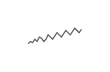
\begin{tikzpicture}[x=0.08em, y=0.08em, line width=0.4pt]
                \draw[FooterGray] (0,3) -- (1,4) -- (2,3.5) -- (3,5) -- (4,4) -- (5,6) -- (6,5.5) -- (7,4) -- (8,5) -- (9,7) -- (10,6) -- (11,5) -- (12,6.5) -- (13,8) -- (14,7) -- (15,6) -- (16,7.5) -- (17,9) -- (18,8) -- (19,7) -- (20,8.5) -- (21,10) -- (22,9) -- (23,8) -- (24,9.5);
            \end{tikzpicture}%
        }%
        \hskip0.5cm%
    }%
    \vskip6pt%
}

%=============================================================================
% PACKAGES
%=============================================================================
\usepackage[utf8]{inputenc}
\DeclareUnicodeCharacter{03B1}{\ensuremath{\alpha}}
\usepackage[T1]{fontenc}
\usepackage{amsmath, amssymb, amsthm}
\usepackage{mathtools}
\usepackage{bm}
\usepackage{tikz}
\usetikzlibrary{arrows.meta, positioning, shapes, calc, decorations.pathreplacing, shadings}
\usepackage{booktabs}
\usepackage{multirow}
\usepackage{array}
\usepackage{graphicx}
\usepackage{animate}
\usepackage{hyperref}
\usepackage{colortbl}
\usepackage{listings}
\lstset{language=Python, basicstyle=\ttfamily\scriptsize, keywordstyle=\color{MainBlue}\bfseries,
  commentstyle=\color{Forest}, stringstyle=\color{Crimson}, breaklines=true,
  frame=none, backgroundcolor=\color{VeryLightGray}, xleftmargin=2mm}
\hypersetup{colorlinks=true, linkcolor=MainBlue, urlcolor=MainBlue}
\graphicspath{{../../logos/}{../../charts/}{../../photos/}}
\usepackage{xcolor}
\hfuzz=2pt  % Suppress tiny overfull warnings (<2pt)
\vfuzz=2pt  % Suppress tiny vertical overfull warnings (<2pt)
% \mathrm in the sans-serif family of the slides (beamer resets \mathrm to the serif family at \begin{document};
% this hook runs after beamer's, so WN, Var, RMSE, ... in formulas match the surrounding text)
% Bold vectors and matrices in the same sans-serif family: \mathbf{A} in sans bold (beamer's own \mathbf came out in
% medium weight), and the bold upright Greek capitals of \boldsymbol / \bm (\bSigma, \bPhi, \boldsymbol{\Theta}) in
% cmss bold: bm.sty fixes its "boldoperators" font when it is loaded (serif cmbx), before beamer switches the
% operators to cmss, so it is reset here.
\AtBeginDocument{%
  \SetMathAlphabet{\mathrm}{normal}{\encodingdefault}{\sfdefault}{\mddefault}{n}%
  \SetMathAlphabet{\mathrm}{bold}{\encodingdefault}{\sfdefault}{bx}{n}%
  \SetMathAlphabet{\mathbf}{normal}{\encodingdefault}{\sfdefault}{bx}{n}%
  \SetMathAlphabet{\mathbf}{bold}{\encodingdefault}{\sfdefault}{bx}{n}%
  \SetSymbolFont{boldoperators}{normal}{OT1}{cmss}{bx}{n}%
  \SetSymbolFont{boldoperators}{bold}{OT1}{cmss}{bx}{n}}

%=============================================================================
% QUANTLET COMMANDS
%   \quantlet{<displayed name>}{<url>}       (generic, compatible with the older TSA decks)
%   \tsaquantlet{Ch_05}{TSA_ch5_garch}       -> https://github.com/danpele/Time-Series-Analysis/tree/main/Quantlets/Ch_05/TSA_ch5_garch
%   \qlurl{<folder>} is defined per chapter by the generator (Quantlets/Ch_NN/<folder>)
%=============================================================================
\newcommand{\tsarepo}{https://github.com/danpele/Time-Series-Analysis}
\newcommand{\tsaqlbase}{https://github.com/danpele/Time-Series-Analysis/tree/main/Quantlets}
\newcommand{\quantlet}[2]{%
    \hfill\href{#2}{%
        \raisebox{-0.15em}{
\includegraphics[height=0.7em]{ql_logo.png}}%
        \textcolor{MainBlue}{\tiny\ #1}%
    }%
}
\newcommand{\tsaquantlet}[2]{\quantlet{\detokenize{#2}}{\tsaqlbase/#1/#2}}

%=============================================================================
% NOTEBOOKS (Google Colab)
%   \colaburl{notebooks/EN/chapter5_seminar_notebook.ipynb} -> the Colab link of a file in the TSA repo
%   \nb: the chapter notebook (each seminar deck redefines it with \renewcommand)
%=============================================================================
\newcommand{\colaburl}[1]{https://colab.research.google.com/github/danpele/Time-Series-Analysis/blob/main/#1}
\newcommand{\nb}{https://colab.research.google.com/github/danpele/Time-Series-Analysis/tree/main/notebooks/EN}
\newcommand{\nbname}{notebooks/EN}

%=============================================================================
% SLIDE HELPERS (used by the generators; the same as in MFM)
%=============================================================================
% local font size for list bodies (the preamble forces \normalsize)
\newcommand{\itemsize}[1]{\setbeamertemplate{itemize/enumerate body begin}{#1}\setbeamertemplate{itemize/enumerate subbody begin}{#1}}
\newcommand{\intitle}[1]{{\hypersetup{urlcolor=white}#1}}   % white links inside coloured title bars
\newcommand{\imgcap}[1]{{\scriptsize #1}\\[0.5mm]}          % caption under a photo
\newcommand{\imgcredit}[2]{{\tiny\color{FooterGray}\href{#1}{#2}}}   % image credit: source URL, author/licence
\newcommand{\aiprompt}[1]{{\ttfamily\color{MainBlue}#1}}     % a prompt to an AI assistant

%=============================================================================
% SEMINARS: student version by default; the instructor wrapper *_solutions.tex sets \solutionstrue
%=============================================================================
\makeatletter\@ifundefined{ifsolutions}{\expandafter\newif\csname ifsolutions\endcsname}{}\makeatother
\newcommand{\solonly}[1]{\ifsolutions #1\fi}
\newcommand{\propsub}{\ifsolutions\else\framesubtitle{\ifdefined\tsalang Rezolvarea se discută la seminar\else Solution discussed in class\fi}\fi}

%=============================================================================
% APPENDIX AND CHAPTER LINKS (latex/appendix_links.py writes the calls; it also re-declares these
% macros before \begin{document}, so the decks compile with or without this preamble block)
%=============================================================================
\providecommand{\tsaapplink}[3]{\hypertarget{#2}{}\hyperlink{#1}{\beamergotobutton{#3}}}
\providecommand{\tsaappback}[2]{\begin{tikzpicture}[remember picture,overlay]\node[anchor=south east] at ([xshift=-3mm,yshift=7mm]current page.south east){\hyperlink{#1}{\beamerreturnbutton{#2}}};\end{tikzpicture}}
\providecommand{\tsachlink}[2]{\href{#1}{#2}}
\providecommand{\tsachlinkt}[2]{\href{#1}{\usebeamercolor[fg]{frametitle}#2}}

%=============================================================================
% QUANTINAR COMMAND: link către un curs Quantinar (subiecte avansate)
%=============================================================================
\newcommand{\quantinar}[2]{%
    \href{#2}{%
        \raisebox{-0.15em}{
\includegraphics[height=0.8em]{qr_logo.png}}%
        \textcolor{MainBlue}{\scriptsize\ #1}%
    }%
}

%=============================================================================
% CUSTOM TITLE PAGE
%=============================================================================
\defbeamertemplate*{title page}{hybrid}[1][]
{
    \vspace{0.2cm}
    % Logos row - top header (with clickable links)
    \begin{center}
        \href{https://www.ase.ro}{
\includegraphics[height=1.0cm]{ase_logo.png}}\hspace{0.3cm}%
        \href{https://theida.net}{
\includegraphics[height=1.0cm]{ida_logo.png}}\hspace{0.3cm}%
        \href{https://blockchain-research-center.com}{
\includegraphics[height=1.0cm]{brc_logo.png}}\hspace{0.3cm}%
        \href{https://www.ai4efin.ase.ro}{
\includegraphics[height=1.0cm]{ai4efin_logo.png}}\hspace{0.3cm}%
        \href{https://ipe.ro/new}{
\includegraphics[height=1.0cm]{acad_logo.png}}\hspace{0.3cm}%
        \href{https://www.digital-finance-msca.com}{
\includegraphics[height=1.0cm]{msca_logo.png}}%
    \end{center}

    \vspace{0.6cm}

    % Main title with Q logos on sides (with clickable links)
    \begin{center}
        \begin{minipage}{0.1\textwidth}
            \centering
            \href{https://quantlet.com}{
\includegraphics[height=1.1cm]{ql_logo.png}}
        \end{minipage}%
        \begin{minipage}{0.78\textwidth}
            \centering
            {\LARGE\bfseries\usebeamercolor[fg]{title}\inserttitle}

            \vspace{0.3cm}

            {\usebeamerfont{subtitle}\usebeamercolor[fg]{title}\insertsubtitle}
        \end{minipage}%
        \begin{minipage}{0.1\textwidth}
            \centering
            \href{https://quantinar.com}{
\includegraphics[height=1.1cm]{qr_logo.png}}
        \end{minipage}
    \end{center}

    \vspace{0.6cm}

    % Authors (left aligned)
    \hspace{0.5cm}{\usebeamerfont{author}\insertauthor}

    \vspace{0.3cm}

    % Institute/Affiliations (left aligned)
    \hspace{0.5cm}\begin{minipage}[t]{0.9\textwidth}
        \raggedright\small\insertinstitute
    \end{minipage}
}

%=============================================================================
% THEOREM ENVIRONMENTS
%=============================================================================
\theoremstyle{definition}
\setbeamertemplate{theorems}[numbered]
\ifdefined\tsalang
\newtheorem{defn}{Definiție}
\newtheorem{thm}{Teoremă}
\newtheorem{prop}{Propoziție}
\newtheorem{rmk}{Observație}
\else
\newtheorem{defn}{Definition}
\newtheorem{thm}{Theorem}
\newtheorem{prop}{Proposition}
\newtheorem{rmk}{Remark}
\fi

%=============================================================================
% CENTRED MINIPAGE (no extra vertical space)
%=============================================================================
\newenvironment{cminipage}[1]{%
    \par\noindent\hfill\begin{minipage}{#1}\ignorespaces
}{%
    \end{minipage}\hfill\null\par
}

%=============================================================================
% CUSTOM COMMANDS
%=============================================================================
\newcommand{\E}{\mathbb{E}}
\newcommand{\Var}{\text{Var}}
\newcommand{\Cov}{\text{Cov}}
\newcommand{\Corr}{\text{Corr}}
\newcommand{\R}{\mathbb{R}}
\newcommand{\N}{\mathbb{N}}
\newcommand{\Z}{\mathbb{Z}}
\newcommand{\B}{\mathbf{B}}
\newcommand{\imark}{\textcolor{MainBlue}{\textbullet}}
\newcommand{\RMSE}{\text{RMSE}}
\newcommand{\MAE}{\text{MAE}}
\newcommand{\MAPE}{\text{MAPE}}

% Boldface vector/matrix commands (VAR, VECM, state space; also used by the older TSA decks)
\newcommand{\bY}{\mathbf{Y}}
\newcommand{\bX}{\mathbf{X}}
\newcommand{\bA}{\mathbf{A}}
\newcommand{\bB}{\mathbf{B}}
\newcommand{\bepsilon}{\boldsymbol{\varepsilon}}
\newcommand{\bSigma}{\boldsymbol{\Sigma}}
\newcommand{\bPhi}{\boldsymbol{\Phi}}
\newcommand{\bGamma}{\boldsymbol{\Gamma}}
\newcommand{\bPi}{\boldsymbol{\Pi}}
\newcommand{\bc}{\mathbf{c}}
\newcommand{\balpha}{\boldsymbol{\alpha}}
\newcommand{\bbeta}{\boldsymbol{\beta}}
\newcommand{\bvarepsilon}{\boldsymbol{\varepsilon}}

% Legacy seminar marks (older TSA seminar decks)
\newcommand{\correct}{\textcolor{Forest}{\checkmark}}
\newcommand{\incorrect}{\textcolor{Crimson}{\texttimes}}
 se definește
%   \newcommand{\coursename}{Time Series Analysis}      (EN)
%   \newcommand{\coursename}{Serii de timp}       (RO)  și  \def\tsalang{ro}
% Fișierele .tex se află în EN/Courses, EN/Seminars, RO/Cursuri, RO/Seminarii (două niveluri sub rădăcină).
% Deck-urile sînt generate de latex/build_chapterN.py / build_seminarN.py (vezi latex/tsa_build.py).

\documentclass[9pt, aspectratio=169, t]{beamer}
\providecommand{\coursename}{Time Series Analysis}

% Ensure content fits on slides
\setbeamersize{text margin left=8mm, text margin right=8mm}
% Smaller institute font (title page)
\setbeamerfont{institute}{size=\footnotesize}

%=============================================================================
% THEME AND STYLE CONFIGURATION
%=============================================================================
\usetheme{default}
% Using default theme for clean header/footer control

% Color Palette (matching Redispatch PDF)
\definecolor{MainBlue}{RGB}{26, 58, 110}
\definecolor{AccentBlue}{RGB}{26, 58, 110}
\definecolor{IDAred}{RGB}{205, 0, 0}
\definecolor{DarkGray}{RGB}{51, 51, 51}
\definecolor{MediumGray}{RGB}{128, 128, 128}
\definecolor{LightGray}{RGB}{248, 248, 248}
\definecolor{VeryLightGray}{RGB}{235, 235, 235}
\definecolor{KeynoteGray}{RGB}{218, 218, 218}
\definecolor{SectionGray}{RGB}{120, 120, 120}
\definecolor{FooterGray}{RGB}{100, 100, 100}
\definecolor{Crimson}{RGB}{220, 53, 69}
\definecolor{Forest}{RGB}{46, 125, 50}
\definecolor{Amber}{RGB}{181, 133, 63}
\definecolor{Orange}{RGB}{230, 126, 34}
\definecolor{Purple}{RGB}{142, 68, 173}

% Gradient background (exact Keynote 315° gradient: white to RGB 218,218,218)
\setbeamertemplate{background}{%
    \begin{tikzpicture}[remember picture, overlay]
        \shade[shading=axis, shading angle=315,
        top color=white, bottom color=KeynoteGray]
        (current page.south west) rectangle (current page.north east);
    \end{tikzpicture}%
}
% Fallback solid color for compatibility
\setbeamercolor{background canvas}{bg=}

\setbeamercolor{palette primary}{bg=MainBlue, fg=white}
\setbeamercolor{palette secondary}{bg=MainBlue!85, fg=white}
\setbeamercolor{palette tertiary}{bg=MainBlue!70, fg=white}
\setbeamercolor{structure}{fg=MainBlue}
\setbeamercolor{title}{fg=IDAred}
\setbeamercolor{frametitle}{fg=IDAred, bg=}
\setbeamercolor{block title}{bg=MainBlue, fg=white}
\setbeamercolor{block body}{bg=VeryLightGray, fg=DarkGray}
\setbeamercolor{block title alerted}{bg=Crimson, fg=white}
\setbeamercolor{block body alerted}{bg=Crimson!8, fg=DarkGray}
\setbeamercolor{block title example}{bg=Forest, fg=white}
\setbeamercolor{block body example}{bg=Forest!8, fg=DarkGray}
\setbeamercolor{item}{fg=MainBlue}

% Footer colors (override Madrid theme blue)
\setbeamercolor{author in head/foot}{fg=FooterGray, bg=}
\setbeamercolor{title in head/foot}{fg=FooterGray, bg=}
\setbeamercolor{date in head/foot}{fg=FooterGray, bg=}
\setbeamercolor{section in head/foot}{fg=FooterGray, bg=}
\setbeamercolor{subsection in head/foot}{fg=FooterGray, bg=}

% Bullet styles (apply everywhere including blocks)
\setbeamertemplate{itemize item}{\color{MainBlue}$\boxdot$}
\setbeamertemplate{itemize subitem}{\color{MainBlue}$\blacktriangleright$}
\setbeamertemplate{itemize subsubitem}{\color{MainBlue}\tiny$\bullet$}
\setbeamertemplate{itemize/enumerate body begin}{\normalsize}
\setbeamertemplate{itemize/enumerate subbody begin}{\normalsize}

% Item spacing - compact style
\setlength{\leftmargini}{10pt}       % Level 1: minimal indent
\setlength{\leftmarginii}{10pt}      % Level 2: minimal additional indent
% Compact list spacing (zero extra space before/after lists in blocks)
\makeatletter
\def\@listi{\leftmargin\leftmargini \topsep 0pt \parsep 0pt \itemsep 0pt}
\def\@listii{\leftmargin\leftmarginii \topsep 0pt \parsep 0pt \itemsep 0pt}
\makeatother

\setbeamertemplate{navigation symbols}{}

%=============================================================================
% CUSTOM HEADLINE
%=============================================================================
\setbeamertemplate{headline}{%
    \vskip10pt%
    \hbox to \paperwidth{%
        \hskip0.5cm%
        {\small\color{FooterGray}\renewcommand{\hyperlink}[2]{##2}\insertsectionhead}%
        \hfill%
        \textcolor{FooterGray}{\small\insertframenumber}%
        \hskip0.5cm%
    }%
    \vskip4pt%
    {\color{FooterGray}\hrule height 0.4pt}%
}

%=============================================================================
% CUSTOM FOOTER
%=============================================================================
\usepackage{fontawesome5}

\setbeamertemplate{footline}{%
    {\color{FooterGray}\hrule height 0.4pt}%
    \vskip4pt%
    \hbox to \paperwidth{%
        \hskip0.5cm%
        \textcolor{FooterGray}{\small\coursename}%
        \hfill%
        \raisebox{-0.1em}{%
            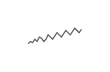
\begin{tikzpicture}[x=0.08em, y=0.08em, line width=0.4pt]
                \draw[FooterGray] (0,3) -- (1,4) -- (2,3.5) -- (3,5) -- (4,4) -- (5,6) -- (6,5.5) -- (7,4) -- (8,5) -- (9,7) -- (10,6) -- (11,5) -- (12,6.5) -- (13,8) -- (14,7) -- (15,6) -- (16,7.5) -- (17,9) -- (18,8) -- (19,7) -- (20,8.5) -- (21,10) -- (22,9) -- (23,8) -- (24,9.5);
            \end{tikzpicture}%
        }%
        \hskip0.5cm%
    }%
    \vskip6pt%
}

%=============================================================================
% PACKAGES
%=============================================================================
\usepackage[utf8]{inputenc}
\DeclareUnicodeCharacter{03B1}{\ensuremath{\alpha}}
\usepackage[T1]{fontenc}
\usepackage{amsmath, amssymb, amsthm}
\usepackage{mathtools}
\usepackage{bm}
\usepackage{tikz}
\usetikzlibrary{arrows.meta, positioning, shapes, calc, decorations.pathreplacing, shadings}
\usepackage{booktabs}
\usepackage{multirow}
\usepackage{array}
\usepackage{graphicx}
\usepackage{animate}
\usepackage{hyperref}
\usepackage{colortbl}
\usepackage{listings}
\lstset{language=Python, basicstyle=\ttfamily\scriptsize, keywordstyle=\color{MainBlue}\bfseries,
  commentstyle=\color{Forest}, stringstyle=\color{Crimson}, breaklines=true,
  frame=none, backgroundcolor=\color{VeryLightGray}, xleftmargin=2mm}
\hypersetup{colorlinks=true, linkcolor=MainBlue, urlcolor=MainBlue}
\graphicspath{{../../logos/}{../../charts/}{../../photos/}}
\usepackage{xcolor}
\hfuzz=2pt  % Suppress tiny overfull warnings (<2pt)
\vfuzz=2pt  % Suppress tiny vertical overfull warnings (<2pt)
% \mathrm in the sans-serif family of the slides (beamer resets \mathrm to the serif family at \begin{document};
% this hook runs after beamer's, so WN, Var, RMSE, ... in formulas match the surrounding text)
% Bold vectors and matrices in the same sans-serif family: \mathbf{A} in sans bold (beamer's own \mathbf came out in
% medium weight), and the bold upright Greek capitals of \boldsymbol / \bm (\bSigma, \bPhi, \boldsymbol{\Theta}) in
% cmss bold: bm.sty fixes its "boldoperators" font when it is loaded (serif cmbx), before beamer switches the
% operators to cmss, so it is reset here.
\AtBeginDocument{%
  \SetMathAlphabet{\mathrm}{normal}{\encodingdefault}{\sfdefault}{\mddefault}{n}%
  \SetMathAlphabet{\mathrm}{bold}{\encodingdefault}{\sfdefault}{bx}{n}%
  \SetMathAlphabet{\mathbf}{normal}{\encodingdefault}{\sfdefault}{bx}{n}%
  \SetMathAlphabet{\mathbf}{bold}{\encodingdefault}{\sfdefault}{bx}{n}%
  \SetSymbolFont{boldoperators}{normal}{OT1}{cmss}{bx}{n}%
  \SetSymbolFont{boldoperators}{bold}{OT1}{cmss}{bx}{n}}

%=============================================================================
% QUANTLET COMMANDS
%   \quantlet{<displayed name>}{<url>}       (generic, compatible with the older TSA decks)
%   \tsaquantlet{Ch_05}{TSA_ch5_garch}       -> https://github.com/danpele/Time-Series-Analysis/tree/main/Quantlets/Ch_05/TSA_ch5_garch
%   \qlurl{<folder>} is defined per chapter by the generator (Quantlets/Ch_NN/<folder>)
%=============================================================================
\newcommand{\tsarepo}{https://github.com/danpele/Time-Series-Analysis}
\newcommand{\tsaqlbase}{https://github.com/danpele/Time-Series-Analysis/tree/main/Quantlets}
\newcommand{\quantlet}[2]{%
    \hfill\href{#2}{%
        \raisebox{-0.15em}{
\includegraphics[height=0.7em]{ql_logo.png}}%
        \textcolor{MainBlue}{\tiny\ #1}%
    }%
}
\newcommand{\tsaquantlet}[2]{\quantlet{\detokenize{#2}}{\tsaqlbase/#1/#2}}

%=============================================================================
% NOTEBOOKS (Google Colab)
%   \colaburl{notebooks/EN/chapter5_seminar_notebook.ipynb} -> the Colab link of a file in the TSA repo
%   \nb: the chapter notebook (each seminar deck redefines it with \renewcommand)
%=============================================================================
\newcommand{\colaburl}[1]{https://colab.research.google.com/github/danpele/Time-Series-Analysis/blob/main/#1}
\newcommand{\nb}{https://colab.research.google.com/github/danpele/Time-Series-Analysis/tree/main/notebooks/EN}
\newcommand{\nbname}{notebooks/EN}

%=============================================================================
% SLIDE HELPERS (used by the generators; the same as in MFM)
%=============================================================================
% local font size for list bodies (the preamble forces \normalsize)
\newcommand{\itemsize}[1]{\setbeamertemplate{itemize/enumerate body begin}{#1}\setbeamertemplate{itemize/enumerate subbody begin}{#1}}
\newcommand{\intitle}[1]{{\hypersetup{urlcolor=white}#1}}   % white links inside coloured title bars
\newcommand{\imgcap}[1]{{\scriptsize #1}\\[0.5mm]}          % caption under a photo
\newcommand{\imgcredit}[2]{{\tiny\color{FooterGray}\href{#1}{#2}}}   % image credit: source URL, author/licence
\newcommand{\aiprompt}[1]{{\ttfamily\color{MainBlue}#1}}     % a prompt to an AI assistant

%=============================================================================
% SEMINARS: student version by default; the instructor wrapper *_solutions.tex sets \solutionstrue
%=============================================================================
\makeatletter\@ifundefined{ifsolutions}{\expandafter\newif\csname ifsolutions\endcsname}{}\makeatother
\newcommand{\solonly}[1]{\ifsolutions #1\fi}
\newcommand{\propsub}{\ifsolutions\else\framesubtitle{\ifdefined\tsalang Rezolvarea se discută la seminar\else Solution discussed in class\fi}\fi}

%=============================================================================
% APPENDIX AND CHAPTER LINKS (latex/appendix_links.py writes the calls; it also re-declares these
% macros before \begin{document}, so the decks compile with or without this preamble block)
%=============================================================================
\providecommand{\tsaapplink}[3]{\hypertarget{#2}{}\hyperlink{#1}{\beamergotobutton{#3}}}
\providecommand{\tsaappback}[2]{\begin{tikzpicture}[remember picture,overlay]\node[anchor=south east] at ([xshift=-3mm,yshift=7mm]current page.south east){\hyperlink{#1}{\beamerreturnbutton{#2}}};\end{tikzpicture}}
\providecommand{\tsachlink}[2]{\href{#1}{#2}}
\providecommand{\tsachlinkt}[2]{\href{#1}{\usebeamercolor[fg]{frametitle}#2}}

%=============================================================================
% QUANTINAR COMMAND: link către un curs Quantinar (subiecte avansate)
%=============================================================================
\newcommand{\quantinar}[2]{%
    \href{#2}{%
        \raisebox{-0.15em}{
\includegraphics[height=0.8em]{qr_logo.png}}%
        \textcolor{MainBlue}{\scriptsize\ #1}%
    }%
}

%=============================================================================
% CUSTOM TITLE PAGE
%=============================================================================
\defbeamertemplate*{title page}{hybrid}[1][]
{
    \vspace{0.2cm}
    % Logos row - top header (with clickable links)
    \begin{center}
        \href{https://www.ase.ro}{
\includegraphics[height=1.0cm]{ase_logo.png}}\hspace{0.3cm}%
        \href{https://theida.net}{
\includegraphics[height=1.0cm]{ida_logo.png}}\hspace{0.3cm}%
        \href{https://blockchain-research-center.com}{
\includegraphics[height=1.0cm]{brc_logo.png}}\hspace{0.3cm}%
        \href{https://www.ai4efin.ase.ro}{
\includegraphics[height=1.0cm]{ai4efin_logo.png}}\hspace{0.3cm}%
        \href{https://ipe.ro/new}{
\includegraphics[height=1.0cm]{acad_logo.png}}\hspace{0.3cm}%
        \href{https://www.digital-finance-msca.com}{
\includegraphics[height=1.0cm]{msca_logo.png}}%
    \end{center}

    \vspace{0.6cm}

    % Main title with Q logos on sides (with clickable links)
    \begin{center}
        \begin{minipage}{0.1\textwidth}
            \centering
            \href{https://quantlet.com}{
\includegraphics[height=1.1cm]{ql_logo.png}}
        \end{minipage}%
        \begin{minipage}{0.78\textwidth}
            \centering
            {\LARGE\bfseries\usebeamercolor[fg]{title}\inserttitle}

            \vspace{0.3cm}

            {\usebeamerfont{subtitle}\usebeamercolor[fg]{title}\insertsubtitle}
        \end{minipage}%
        \begin{minipage}{0.1\textwidth}
            \centering
            \href{https://quantinar.com}{
\includegraphics[height=1.1cm]{qr_logo.png}}
        \end{minipage}
    \end{center}

    \vspace{0.6cm}

    % Authors (left aligned)
    \hspace{0.5cm}{\usebeamerfont{author}\insertauthor}

    \vspace{0.3cm}

    % Institute/Affiliations (left aligned)
    \hspace{0.5cm}\begin{minipage}[t]{0.9\textwidth}
        \raggedright\small\insertinstitute
    \end{minipage}
}

%=============================================================================
% THEOREM ENVIRONMENTS
%=============================================================================
\theoremstyle{definition}
\setbeamertemplate{theorems}[numbered]
\ifdefined\tsalang
\newtheorem{defn}{Definiție}
\newtheorem{thm}{Teoremă}
\newtheorem{prop}{Propoziție}
\newtheorem{rmk}{Observație}
\else
\newtheorem{defn}{Definition}
\newtheorem{thm}{Theorem}
\newtheorem{prop}{Proposition}
\newtheorem{rmk}{Remark}
\fi

%=============================================================================
% CENTRED MINIPAGE (no extra vertical space)
%=============================================================================
\newenvironment{cminipage}[1]{%
    \par\noindent\hfill\begin{minipage}{#1}\ignorespaces
}{%
    \end{minipage}\hfill\null\par
}

%=============================================================================
% CUSTOM COMMANDS
%=============================================================================
\newcommand{\E}{\mathbb{E}}
\newcommand{\Var}{\text{Var}}
\newcommand{\Cov}{\text{Cov}}
\newcommand{\Corr}{\text{Corr}}
\newcommand{\R}{\mathbb{R}}
\newcommand{\N}{\mathbb{N}}
\newcommand{\Z}{\mathbb{Z}}
\newcommand{\B}{\mathbf{B}}
\newcommand{\imark}{\textcolor{MainBlue}{\textbullet}}
\newcommand{\RMSE}{\text{RMSE}}
\newcommand{\MAE}{\text{MAE}}
\newcommand{\MAPE}{\text{MAPE}}

% Boldface vector/matrix commands (VAR, VECM, state space; also used by the older TSA decks)
\newcommand{\bY}{\mathbf{Y}}
\newcommand{\bX}{\mathbf{X}}
\newcommand{\bA}{\mathbf{A}}
\newcommand{\bB}{\mathbf{B}}
\newcommand{\bepsilon}{\boldsymbol{\varepsilon}}
\newcommand{\bSigma}{\boldsymbol{\Sigma}}
\newcommand{\bPhi}{\boldsymbol{\Phi}}
\newcommand{\bGamma}{\boldsymbol{\Gamma}}
\newcommand{\bPi}{\boldsymbol{\Pi}}
\newcommand{\bc}{\mathbf{c}}
\newcommand{\balpha}{\boldsymbol{\alpha}}
\newcommand{\bbeta}{\boldsymbol{\beta}}
\newcommand{\bvarepsilon}{\boldsymbol{\varepsilon}}

% Legacy seminar marks (older TSA seminar decks)
\newcommand{\correct}{\textcolor{Forest}{\checkmark}}
\newcommand{\incorrect}{\textcolor{Crimson}{\texttimes}}
 se definește
%   \newcommand{\coursename}{Time Series Analysis}      (EN)
%   \newcommand{\coursename}{Serii de timp}       (RO)  și  \def\tsalang{ro}
% Fișierele .tex se află în EN/Courses, EN/Seminars, RO/Cursuri, RO/Seminarii (două niveluri sub rădăcină).
% Deck-urile sînt generate de latex/build_chapterN.py / build_seminarN.py (vezi latex/tsa_build.py).

\documentclass[9pt, aspectratio=169, t]{beamer}
\providecommand{\coursename}{Time Series Analysis}

% Ensure content fits on slides
\setbeamersize{text margin left=8mm, text margin right=8mm}
% Smaller institute font (title page)
\setbeamerfont{institute}{size=\footnotesize}

%=============================================================================
% THEME AND STYLE CONFIGURATION
%=============================================================================
\usetheme{default}
% Using default theme for clean header/footer control

% Color Palette (matching Redispatch PDF)
\definecolor{MainBlue}{RGB}{26, 58, 110}
\definecolor{AccentBlue}{RGB}{26, 58, 110}
\definecolor{IDAred}{RGB}{205, 0, 0}
\definecolor{DarkGray}{RGB}{51, 51, 51}
\definecolor{MediumGray}{RGB}{128, 128, 128}
\definecolor{LightGray}{RGB}{248, 248, 248}
\definecolor{VeryLightGray}{RGB}{235, 235, 235}
\definecolor{KeynoteGray}{RGB}{218, 218, 218}
\definecolor{SectionGray}{RGB}{120, 120, 120}
\definecolor{FooterGray}{RGB}{100, 100, 100}
\definecolor{Crimson}{RGB}{220, 53, 69}
\definecolor{Forest}{RGB}{46, 125, 50}
\definecolor{Amber}{RGB}{181, 133, 63}
\definecolor{Orange}{RGB}{230, 126, 34}
\definecolor{Purple}{RGB}{142, 68, 173}

% Gradient background (exact Keynote 315° gradient: white to RGB 218,218,218)
\setbeamertemplate{background}{%
    \begin{tikzpicture}[remember picture, overlay]
        \shade[shading=axis, shading angle=315,
        top color=white, bottom color=KeynoteGray]
        (current page.south west) rectangle (current page.north east);
    \end{tikzpicture}%
}
% Fallback solid color for compatibility
\setbeamercolor{background canvas}{bg=}

\setbeamercolor{palette primary}{bg=MainBlue, fg=white}
\setbeamercolor{palette secondary}{bg=MainBlue!85, fg=white}
\setbeamercolor{palette tertiary}{bg=MainBlue!70, fg=white}
\setbeamercolor{structure}{fg=MainBlue}
\setbeamercolor{title}{fg=IDAred}
\setbeamercolor{frametitle}{fg=IDAred, bg=}
\setbeamercolor{block title}{bg=MainBlue, fg=white}
\setbeamercolor{block body}{bg=VeryLightGray, fg=DarkGray}
\setbeamercolor{block title alerted}{bg=Crimson, fg=white}
\setbeamercolor{block body alerted}{bg=Crimson!8, fg=DarkGray}
\setbeamercolor{block title example}{bg=Forest, fg=white}
\setbeamercolor{block body example}{bg=Forest!8, fg=DarkGray}
\setbeamercolor{item}{fg=MainBlue}

% Footer colors (override Madrid theme blue)
\setbeamercolor{author in head/foot}{fg=FooterGray, bg=}
\setbeamercolor{title in head/foot}{fg=FooterGray, bg=}
\setbeamercolor{date in head/foot}{fg=FooterGray, bg=}
\setbeamercolor{section in head/foot}{fg=FooterGray, bg=}
\setbeamercolor{subsection in head/foot}{fg=FooterGray, bg=}

% Bullet styles (apply everywhere including blocks)
\setbeamertemplate{itemize item}{\color{MainBlue}$\boxdot$}
\setbeamertemplate{itemize subitem}{\color{MainBlue}$\blacktriangleright$}
\setbeamertemplate{itemize subsubitem}{\color{MainBlue}\tiny$\bullet$}
\setbeamertemplate{itemize/enumerate body begin}{\normalsize}
\setbeamertemplate{itemize/enumerate subbody begin}{\normalsize}

% Item spacing - compact style
\setlength{\leftmargini}{10pt}       % Level 1: minimal indent
\setlength{\leftmarginii}{10pt}      % Level 2: minimal additional indent
% Compact list spacing (zero extra space before/after lists in blocks)
\makeatletter
\def\@listi{\leftmargin\leftmargini \topsep 0pt \parsep 0pt \itemsep 0pt}
\def\@listii{\leftmargin\leftmarginii \topsep 0pt \parsep 0pt \itemsep 0pt}
\makeatother

\setbeamertemplate{navigation symbols}{}

%=============================================================================
% CUSTOM HEADLINE
%=============================================================================
\setbeamertemplate{headline}{%
    \vskip10pt%
    \hbox to \paperwidth{%
        \hskip0.5cm%
        {\small\color{FooterGray}\renewcommand{\hyperlink}[2]{##2}\insertsectionhead}%
        \hfill%
        \textcolor{FooterGray}{\small\insertframenumber}%
        \hskip0.5cm%
    }%
    \vskip4pt%
    {\color{FooterGray}\hrule height 0.4pt}%
}

%=============================================================================
% CUSTOM FOOTER
%=============================================================================
\usepackage{fontawesome5}

\setbeamertemplate{footline}{%
    {\color{FooterGray}\hrule height 0.4pt}%
    \vskip4pt%
    \hbox to \paperwidth{%
        \hskip0.5cm%
        \textcolor{FooterGray}{\small\coursename}%
        \hfill%
        \raisebox{-0.1em}{%
            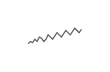
\begin{tikzpicture}[x=0.08em, y=0.08em, line width=0.4pt]
                \draw[FooterGray] (0,3) -- (1,4) -- (2,3.5) -- (3,5) -- (4,4) -- (5,6) -- (6,5.5) -- (7,4) -- (8,5) -- (9,7) -- (10,6) -- (11,5) -- (12,6.5) -- (13,8) -- (14,7) -- (15,6) -- (16,7.5) -- (17,9) -- (18,8) -- (19,7) -- (20,8.5) -- (21,10) -- (22,9) -- (23,8) -- (24,9.5);
            \end{tikzpicture}%
        }%
        \hskip0.5cm%
    }%
    \vskip6pt%
}

%=============================================================================
% PACKAGES
%=============================================================================
\usepackage[utf8]{inputenc}
\DeclareUnicodeCharacter{03B1}{\ensuremath{\alpha}}
\usepackage[T1]{fontenc}
\usepackage{amsmath, amssymb, amsthm}
\usepackage{mathtools}
\usepackage{bm}
\usepackage{tikz}
\usetikzlibrary{arrows.meta, positioning, shapes, calc, decorations.pathreplacing, shadings}
\usepackage{booktabs}
\usepackage{multirow}
\usepackage{array}
\usepackage{graphicx}
\usepackage{animate}
\usepackage{hyperref}
\usepackage{colortbl}
\usepackage{listings}
\lstset{language=Python, basicstyle=\ttfamily\scriptsize, keywordstyle=\color{MainBlue}\bfseries,
  commentstyle=\color{Forest}, stringstyle=\color{Crimson}, breaklines=true,
  frame=none, backgroundcolor=\color{VeryLightGray}, xleftmargin=2mm}
\hypersetup{colorlinks=true, linkcolor=MainBlue, urlcolor=MainBlue}
\graphicspath{{../../logos/}{../../charts/}{../../photos/}}
\usepackage{xcolor}
\hfuzz=2pt  % Suppress tiny overfull warnings (<2pt)
\vfuzz=2pt  % Suppress tiny vertical overfull warnings (<2pt)
% \mathrm in the sans-serif family of the slides (beamer resets \mathrm to the serif family at \begin{document};
% this hook runs after beamer's, so WN, Var, RMSE, ... in formulas match the surrounding text)
% Bold vectors and matrices in the same sans-serif family: \mathbf{A} in sans bold (beamer's own \mathbf came out in
% medium weight), and the bold upright Greek capitals of \boldsymbol / \bm (\bSigma, \bPhi, \boldsymbol{\Theta}) in
% cmss bold: bm.sty fixes its "boldoperators" font when it is loaded (serif cmbx), before beamer switches the
% operators to cmss, so it is reset here.
\AtBeginDocument{%
  \SetMathAlphabet{\mathrm}{normal}{\encodingdefault}{\sfdefault}{\mddefault}{n}%
  \SetMathAlphabet{\mathrm}{bold}{\encodingdefault}{\sfdefault}{bx}{n}%
  \SetMathAlphabet{\mathbf}{normal}{\encodingdefault}{\sfdefault}{bx}{n}%
  \SetMathAlphabet{\mathbf}{bold}{\encodingdefault}{\sfdefault}{bx}{n}%
  \SetSymbolFont{boldoperators}{normal}{OT1}{cmss}{bx}{n}%
  \SetSymbolFont{boldoperators}{bold}{OT1}{cmss}{bx}{n}}

%=============================================================================
% QUANTLET COMMANDS
%   \quantlet{<displayed name>}{<url>}       (generic, compatible with the older TSA decks)
%   \tsaquantlet{Ch_05}{TSA_ch5_garch}       -> https://github.com/danpele/Time-Series-Analysis/tree/main/Quantlets/Ch_05/TSA_ch5_garch
%   \qlurl{<folder>} is defined per chapter by the generator (Quantlets/Ch_NN/<folder>)
%=============================================================================
\newcommand{\tsarepo}{https://github.com/danpele/Time-Series-Analysis}
\newcommand{\tsaqlbase}{https://github.com/danpele/Time-Series-Analysis/tree/main/Quantlets}
\newcommand{\quantlet}[2]{%
    \hfill\href{#2}{%
        \raisebox{-0.15em}{
\includegraphics[height=0.7em]{ql_logo.png}}%
        \textcolor{MainBlue}{\tiny\ #1}%
    }%
}
\newcommand{\tsaquantlet}[2]{\quantlet{\detokenize{#2}}{\tsaqlbase/#1/#2}}

%=============================================================================
% NOTEBOOKS (Google Colab)
%   \colaburl{notebooks/EN/chapter5_seminar_notebook.ipynb} -> the Colab link of a file in the TSA repo
%   \nb: the chapter notebook (each seminar deck redefines it with \renewcommand)
%=============================================================================
\newcommand{\colaburl}[1]{https://colab.research.google.com/github/danpele/Time-Series-Analysis/blob/main/#1}
\newcommand{\nb}{https://colab.research.google.com/github/danpele/Time-Series-Analysis/tree/main/notebooks/EN}
\newcommand{\nbname}{notebooks/EN}

%=============================================================================
% SLIDE HELPERS (used by the generators; the same as in MFM)
%=============================================================================
% local font size for list bodies (the preamble forces \normalsize)
\newcommand{\itemsize}[1]{\setbeamertemplate{itemize/enumerate body begin}{#1}\setbeamertemplate{itemize/enumerate subbody begin}{#1}}
\newcommand{\intitle}[1]{{\hypersetup{urlcolor=white}#1}}   % white links inside coloured title bars
\newcommand{\imgcap}[1]{{\scriptsize #1}\\[0.5mm]}          % caption under a photo
\newcommand{\imgcredit}[2]{{\tiny\color{FooterGray}\href{#1}{#2}}}   % image credit: source URL, author/licence
\newcommand{\aiprompt}[1]{{\ttfamily\color{MainBlue}#1}}     % a prompt to an AI assistant

%=============================================================================
% SEMINARS: student version by default; the instructor wrapper *_solutions.tex sets \solutionstrue
%=============================================================================
\makeatletter\@ifundefined{ifsolutions}{\expandafter\newif\csname ifsolutions\endcsname}{}\makeatother
\newcommand{\solonly}[1]{\ifsolutions #1\fi}
\newcommand{\propsub}{\ifsolutions\else\framesubtitle{\ifdefined\tsalang Rezolvarea se discută la seminar\else Solution discussed in class\fi}\fi}

%=============================================================================
% APPENDIX AND CHAPTER LINKS (latex/appendix_links.py writes the calls; it also re-declares these
% macros before \begin{document}, so the decks compile with or without this preamble block)
%=============================================================================
\providecommand{\tsaapplink}[3]{\hypertarget{#2}{}\hyperlink{#1}{\beamergotobutton{#3}}}
\providecommand{\tsaappback}[2]{\begin{tikzpicture}[remember picture,overlay]\node[anchor=south east] at ([xshift=-3mm,yshift=7mm]current page.south east){\hyperlink{#1}{\beamerreturnbutton{#2}}};\end{tikzpicture}}
\providecommand{\tsachlink}[2]{\href{#1}{#2}}
\providecommand{\tsachlinkt}[2]{\href{#1}{\usebeamercolor[fg]{frametitle}#2}}

%=============================================================================
% QUANTINAR COMMAND: link către un curs Quantinar (subiecte avansate)
%=============================================================================
\newcommand{\quantinar}[2]{%
    \href{#2}{%
        \raisebox{-0.15em}{
\includegraphics[height=0.8em]{qr_logo.png}}%
        \textcolor{MainBlue}{\scriptsize\ #1}%
    }%
}

%=============================================================================
% CUSTOM TITLE PAGE
%=============================================================================
\defbeamertemplate*{title page}{hybrid}[1][]
{
    \vspace{0.2cm}
    % Logos row - top header (with clickable links)
    \begin{center}
        \href{https://www.ase.ro}{
\includegraphics[height=1.0cm]{ase_logo.png}}\hspace{0.3cm}%
        \href{https://theida.net}{
\includegraphics[height=1.0cm]{ida_logo.png}}\hspace{0.3cm}%
        \href{https://blockchain-research-center.com}{
\includegraphics[height=1.0cm]{brc_logo.png}}\hspace{0.3cm}%
        \href{https://www.ai4efin.ase.ro}{
\includegraphics[height=1.0cm]{ai4efin_logo.png}}\hspace{0.3cm}%
        \href{https://ipe.ro/new}{
\includegraphics[height=1.0cm]{acad_logo.png}}\hspace{0.3cm}%
        \href{https://www.digital-finance-msca.com}{
\includegraphics[height=1.0cm]{msca_logo.png}}%
    \end{center}

    \vspace{0.6cm}

    % Main title with Q logos on sides (with clickable links)
    \begin{center}
        \begin{minipage}{0.1\textwidth}
            \centering
            \href{https://quantlet.com}{
\includegraphics[height=1.1cm]{ql_logo.png}}
        \end{minipage}%
        \begin{minipage}{0.78\textwidth}
            \centering
            {\LARGE\bfseries\usebeamercolor[fg]{title}\inserttitle}

            \vspace{0.3cm}

            {\usebeamerfont{subtitle}\usebeamercolor[fg]{title}\insertsubtitle}
        \end{minipage}%
        \begin{minipage}{0.1\textwidth}
            \centering
            \href{https://quantinar.com}{
\includegraphics[height=1.1cm]{qr_logo.png}}
        \end{minipage}
    \end{center}

    \vspace{0.6cm}

    % Authors (left aligned)
    \hspace{0.5cm}{\usebeamerfont{author}\insertauthor}

    \vspace{0.3cm}

    % Institute/Affiliations (left aligned)
    \hspace{0.5cm}\begin{minipage}[t]{0.9\textwidth}
        \raggedright\small\insertinstitute
    \end{minipage}
}

%=============================================================================
% THEOREM ENVIRONMENTS
%=============================================================================
\theoremstyle{definition}
\setbeamertemplate{theorems}[numbered]
\ifdefined\tsalang
\newtheorem{defn}{Definiție}
\newtheorem{thm}{Teoremă}
\newtheorem{prop}{Propoziție}
\newtheorem{rmk}{Observație}
\else
\newtheorem{defn}{Definition}
\newtheorem{thm}{Theorem}
\newtheorem{prop}{Proposition}
\newtheorem{rmk}{Remark}
\fi

%=============================================================================
% CENTRED MINIPAGE (no extra vertical space)
%=============================================================================
\newenvironment{cminipage}[1]{%
    \par\noindent\hfill\begin{minipage}{#1}\ignorespaces
}{%
    \end{minipage}\hfill\null\par
}

%=============================================================================
% CUSTOM COMMANDS
%=============================================================================
\newcommand{\E}{\mathbb{E}}
\newcommand{\Var}{\text{Var}}
\newcommand{\Cov}{\text{Cov}}
\newcommand{\Corr}{\text{Corr}}
\newcommand{\R}{\mathbb{R}}
\newcommand{\N}{\mathbb{N}}
\newcommand{\Z}{\mathbb{Z}}
\newcommand{\B}{\mathbf{B}}
\newcommand{\imark}{\textcolor{MainBlue}{\textbullet}}
\newcommand{\RMSE}{\text{RMSE}}
\newcommand{\MAE}{\text{MAE}}
\newcommand{\MAPE}{\text{MAPE}}

% Boldface vector/matrix commands (VAR, VECM, state space; also used by the older TSA decks)
\newcommand{\bY}{\mathbf{Y}}
\newcommand{\bX}{\mathbf{X}}
\newcommand{\bA}{\mathbf{A}}
\newcommand{\bB}{\mathbf{B}}
\newcommand{\bepsilon}{\boldsymbol{\varepsilon}}
\newcommand{\bSigma}{\boldsymbol{\Sigma}}
\newcommand{\bPhi}{\boldsymbol{\Phi}}
\newcommand{\bGamma}{\boldsymbol{\Gamma}}
\newcommand{\bPi}{\boldsymbol{\Pi}}
\newcommand{\bc}{\mathbf{c}}
\newcommand{\balpha}{\boldsymbol{\alpha}}
\newcommand{\bbeta}{\boldsymbol{\beta}}
\newcommand{\bvarepsilon}{\boldsymbol{\varepsilon}}

% Legacy seminar marks (older TSA seminar decks)
\newcommand{\correct}{\textcolor{Forest}{\checkmark}}
\newcommand{\incorrect}{\textcolor{Crimson}{\texttimes}}


\newcommand{\qlurl}[1]{https://github.com/danpele/Time-Series-Analysis/tree/main/Quantlets/Ch_00/#1}

% Clickable citations (DOIs verified via Crossref)

\newcommand{\refHP}{\href{https://doi.org/10.1007/978-3-031-13584-2}{Huang \& Petukhina (2022)}}
\newcommand{\refFPP}{\href{https://otexts.com/fpp3/}{Hyndman \& Athanasopoulos (2021)}}
\newcommand{\refBD}{\href{https://doi.org/10.1007/978-3-319-29854-2}{Brockwell \& Davis (2016)}}
\newcommand{\refHamilton}{\href{https://doi.org/10.2307/j.ctv14jx6sm}{Hamilton (1994)}}
\newcommand{\refYuleNonsense}{\href{https://doi.org/10.2307/2341482}{Yule (1926)}}
\newcommand{\refYule}{\href{https://doi.org/10.1098/rsta.1927.0007}{Yule (1927)}}
\newcommand{\refSlutsky}{\href{https://doi.org/10.2307/1907241}{Slutzky (1937)}}
\newcommand{\refKolmogorov}{\href{https://doi.org/10.1007/978-94-011-2260-3_28}{Kolmogorov (1941)}}
\newcommand{\refWiener}{\href{https://doi.org/10.7551/mitpress/2946.001.0001}{Wiener (1949)}}
\newcommand{\refBJ}{\href{https://doi.org/10.1002/9781118619193}{Box \& Jenkins (1970)}}
\newcommand{\refHolt}{\href{https://doi.org/10.1016/j.ijforecast.2003.09.015}{Holt (1957)}}
\newcommand{\refWinters}{\href{https://doi.org/10.1287/mnsc.6.3.324}{Winters (1960)}}
\newcommand{\refGardner}{\href{https://doi.org/10.1002/for.3980040103}{Gardner (1985)}}
\newcommand{\refHKSG}{\href{https://doi.org/10.1016/S0169-2070(01)00110-8}{Hyndman, Koehler, Snyder \& Grose (2002)}}
\newcommand{\refHK}{\href{https://doi.org/10.1016/j.ijforecast.2006.03.001}{Hyndman \& Koehler (2006)}}
\newcommand{\refMthree}{\href{https://doi.org/10.1016/S0169-2070(00)00057-1}{Makridakis \& Hibon (2000)}}
\newcommand{\refMfour}{\href{https://doi.org/10.1016/j.ijforecast.2019.04.014}{Makridakis, Spiliotis \& Assimakopoulos (2020)}}
\newcommand{\refSTL}{\href{https://www.scb.se/contentassets/ca21efb41fee47d293bbee5bf7be7fb3/stl-a-seasonal-trend-decomposition-procedure-based-on-loess.pdf}{Cleveland et al.\ (1990)}}
\newcommand{\refKeeling}{\href{https://doi.org/10.3402/tellusa.v12i2.9366}{Keeling (1960)}}
\newcommand{\refEngle}{\href{https://doi.org/10.2307/1912773}{Engle (1982)}}
\newcommand{\refSims}{\href{https://doi.org/10.2307/1912017}{Sims (1980)}}
\newcommand{\refEG}{\href{https://doi.org/10.2307/1913236}{Engle \& Granger (1987)}}
\newcommand{\refStatsmodels}{\href{https://doi.org/10.25080/Majora-92bf1922-011}{Seabold \& Perktold (2010)}}
\newcommand{\refPandas}{\href{https://doi.org/10.25080/Majora-92bf1922-00a}{McKinney (2010)}}
\newcommand{\refNumpy}{\href{https://doi.org/10.1038/s41586-020-2649-2}{Harris et al.\ (2020)}}

\title[Serii de timp]{Serii de timp}
\subtitle{Capitolul 0: Introducere: componente și netezire exponențială}
\author[D.T. Pele]{Daniel Traian PELE}
\institute{Academia de Studii Economice din București\\
IDA Institute Digital Assets\\
Blockchain Research Center\\
AI4EFin Artificial Intelligence for Energy Finance\\
Academia Română, Institutul de Prognoză Economică\\
MSCA Digital Finance}
\date{}

%=============================================================================
\providecommand{\tsaapplink}[3]{\hypertarget{#2}{}\hyperlink{#1}{\beamergotobutton{#3}}}  % APPLINKS-MACROS
\providecommand{\tsaappback}[2]{\begin{tikzpicture}[remember picture,overlay]\node[anchor=south east] at ([xshift=-3mm,yshift=7mm]current page.south east){\hyperlink{#1}{\beamerreturnbutton{#2}}};\end{tikzpicture}}  % APPLINKS-MACROS
\providecommand{\tsachlink}[2]{\href{#1}{#2}}  % APPLINKS-MACROS
\providecommand{\tsachlinkt}[2]{\href{#1}{\usebeamercolor[fg]{frametitle}#2}}  % APPLINKS-MACROS
\begin{document}
%=============================================================================

{
\setbeamertemplate{headline}{}
\setbeamertemplate{footline}{}
\begin{frame}[noframenumbering]
    \titlepage
\end{frame}
}
% BEGIN-ACRONYMS (generat de latex/acronyms.py; nu editati manual)
\begin{frame}{Acronime folosite în acest material (1/2)}
\setbeamertemplate{itemize/enumerate body begin}{\tiny}
\begin{columns}[T]
\begin{column}{0.49\textwidth}
\begin{itemize}\setlength{\itemsep}{0pt}
    \item \textbf{ACF}: Autocorrelation Function (funcția de autocorelație)
    \item \textbf{AI}: Artificial Intelligence (inteligență artificială)
    \item \textbf{API}: Application Programming Interface (interfață de programare a aplicațiilor)
    \item \textbf{AR}: AutoRegressive (model); in event studies: Abnormal Return (model autoregresiv; în studiile de eveniment: randament anormal)
    \item \textbf{ARCH}: AutoRegressive Conditional Heteroskedasticity (heteroscedasticitate condiționată autoregresivă)
    \item \textbf{ARFIMA}: AutoRegressive Fractionally Integrated Moving Average (model) — model autoregresiv fracționar integrat cu medie mobilă
    \item \textbf{ARIMA}: AutoRegressive Integrated Moving Average (model) — model autoregresiv integrat cu medie mobilă
    \item \textbf{ARMA}: AutoRegressive Moving Average (model) — model autoregresiv cu medie mobilă
    \item \textbf{ASE}: Academia de Studii Economice din București
    \item \textbf{BET}: Bucharest Exchange Trading (index) — indicele de referință al Bursei de Valori București
    \item \textbf{BNR}: Banca Națională a României
    \item \textbf{BVB}: Bursa de Valori București
    \item \textbf{CO2}: Carbon dioxide (dioxid de carbon)
\end{itemize}
\end{column}
\begin{column}{0.49\textwidth}
\begin{itemize}\setlength{\itemsep}{0pt}
    \item \textbf{COVID-19}: COronaVIrus Disease 2019 (boala provocată de coronavirus, 2019)
    \item \textbf{CSIE}: Facultatea de Cibernetică, Statistică și Informatică Economică
    \item \textbf{ECTS}: European Credit Transfer and Accumulation System (sistemul european de credite transferabile)
    \item \textbf{EOD}: End Of Day (daily closing data) — date de sfîrșit de zi, adică prețuri de închidere
    \item \textbf{EODHD}: EOD Historical Data (market-data provider) — furnizor de date de piață
    \item \textbf{ETS}: Error, Trend, Seasonality (exponential smoothing state space models) — eroare, trend, sezonalitate (modele de netezire exponențială)
    \item \textbf{FRED}: Federal Reserve Economic Data (baza de date economice a Rezervei Federale din St. Louis)
    \item \textbf{GARCH}: Generalised AutoRegressive Conditional Heteroskedasticity (heteroscedasticitate condiționată autoregresivă generalizată)
    \item \textbf{HICP}: Harmonised Index of Consumer Prices (indicele armonizat al prețurilor de consum)
    \item \textbf{IAPC}: Indicele armonizat al prețurilor de consum
    \item \textbf{INS}: Institutul Național de Statistică
    \item \textbf{LLM}: Large Language Model (model lingvistic de mari dimensiuni)
    \item \textbf{LOESS}: LOcally Estimated Scatterplot Smoothing (netezire locală prin regresie ponderată)
\end{itemize}
\end{column}
\end{columns}
\end{frame}
\begin{frame}{Acronime folosite în acest material (2/2)}
\setbeamertemplate{itemize/enumerate body begin}{\tiny}
\begin{columns}[T]
\begin{column}{0.49\textwidth}
\begin{itemize}\setlength{\itemsep}{0pt}
    \item \textbf{LPPL}: Log-Periodic Power Law (legea de putere log-periodică)
    \item \textbf{MA}: Moving Average (medie mobilă)
    \item \textbf{MAE}: Mean Absolute Error (eroarea absolută medie)
    \item \textbf{MAPE}: Mean Absolute Percentage Error (eroarea procentuală absolută medie)
    \item \textbf{MASE}: Mean Absolute Scaled Error (eroarea absolută medie scalată)
    \item \textbf{PIB}: Produsul intern brut
    \item \textbf{RMSE}: Root Mean Squared Error (rădăcina erorii pătratice medii)
    \item \textbf{SARIMA}: Seasonal ARIMA (model) — model ARIMA sezonier
    \item \textbf{SES}: Simple Exponential Smoothing (netezire exponențială simplă)
    \item \textbf{STL}: Seasonal and Trend decomposition using Loess (descompunerea în sezonalitate și trend cu Loess)
    \item \textbf{SUA}: Statele Unite ale Americii
    \item \textbf{TBATS}: Trigonometric seasonality, Box–Cox, ARMA errors, Trend, Seasonal components (model) — model cu sezonalitate trigonometrică, transformare Box–Cox, erori ARMA, trend și componente sezoniere
    \item \textbf{TRAMO-SEATS}: Time series Regression with ARIMA noise, Missing values and Outliers; Signal Extraction in ARIMA Time Series (metodă de ajustare sezonieră pe baza modelelor ARIMA)
\end{itemize}
\end{column}
\begin{column}{0.49\textwidth}
\begin{itemize}\setlength{\itemsep}{0pt}
    \item \textbf{TVA}: Taxa pe valoarea adăugată
    \item \textbf{UE}: Uniunea Europeană
    \item \textbf{VAR}: Vector AutoRegression (model vector autoregresiv)
    \item \textbf{VECM}: Vector Error Correction Model (model vectorial cu corecția erorii)
\end{itemize}
\end{column}
\end{columns}
\end{frame}
% END-ACRONYMS

%=============================================================================
\section{Organizarea cursului}
%=============================================================================

\begin{frame}{Traseul acestui capitol}
\itemsize{\footnotesize}
\begin{columns}[T]
\begin{column}{0.47\textwidth}
\begin{itemize}
    \item \textbf{Întrebări de pornire}
    \begin{itemize}
        \item ce este o serie de timp și unde o întîlnim?
        \item ce tipare se repetă în datele economice, financiare, energetice și climatice?
        \item cum prognozăm o serie și de unde știm că prognoza este bună?
    \end{itemize}
    \item \textbf{Partea I}
    \begin{itemize}
        \item organizarea cursului
        \item serii de timp pe date reale și o scurtă istorie
        \item componentele: trend, sezonalitate, ciclu, zgomot
    \end{itemize}
    \item \textbf{Partea a II-a}
    \begin{itemize}
        \item notație, transformări și o primă privire asupra ACF
        \item netezirea exponențială; prognoze și evaluarea lor
        \item instrumente și contribuția posibilă a AI
    \end{itemize}
\end{itemize}
\end{column}
\begin{column}{0.50\textwidth}
\begin{itemize}
    \item \textbf{Rezultatele învățării}: după acest capitol puteți
    \begin{itemize}
        \item explica felul în care este organizat și evaluat cursul
        \item recunoaște într-un grafic trendul, sezonalitatea, ciclul și zgomotul
        \item calcula rate de creștere, o medie mobilă și o autocorelație de selecție
        \item construi prognoze naive și prognoze prin netezire exponențială
        \item evalua prognozele pe un set de test, cu MAE, RMSE și MASE
    \end{itemize}
    \item Seminarul 0 are loc \textbf{înaintea} acestui curs și exersează primele instrumente pe date
\end{itemize}
\end{column}
\end{columns}
\end{frame}

\begin{frame}{Cursul pe scurt}
\itemsize{\footnotesize}
\begin{columns}[T]
\begin{column}{0.56\textwidth}
\begin{itemize}
    \item \textbf{Program}
    \begin{itemize}
        \item Licență, programele Informatică economică și Cibernetică economică, anul III, semestrul 2
        \item Facultatea de Cibernetică, Statistică și Informatică Economică (CSIE), ASE București
        \item 4 credite ECTS; 2 ore de curs și 1 oră de seminar pe săptămînă; anul universitar 2026/2027
    \end{itemize}
    \item \textbf{Curs}
    \begin{itemize}
        \item Prof.\ Daniel Traian Pele, \href{mailto:danpele@ase.ro}{danpele@ase.ro}
    \end{itemize}
    \item \textbf{Cunoștințe necesare}
    \begin{itemize}
        \item probabilități și statistică, econometrie (regresia liniară), Python
    \end{itemize}
    \item \textbf{Site-ul cursului}
    \begin{itemize}
        \item \href{https://danpele.github.io/Time-Series-Analysis/}{danpele.github.io/Time-Series-Analysis}: slide-uri, seminarii, notebook-uri, Quantlets, quiz-uri
    \end{itemize}
\end{itemize}
\end{column}
\begin{column}{0.40\textwidth}
\centering
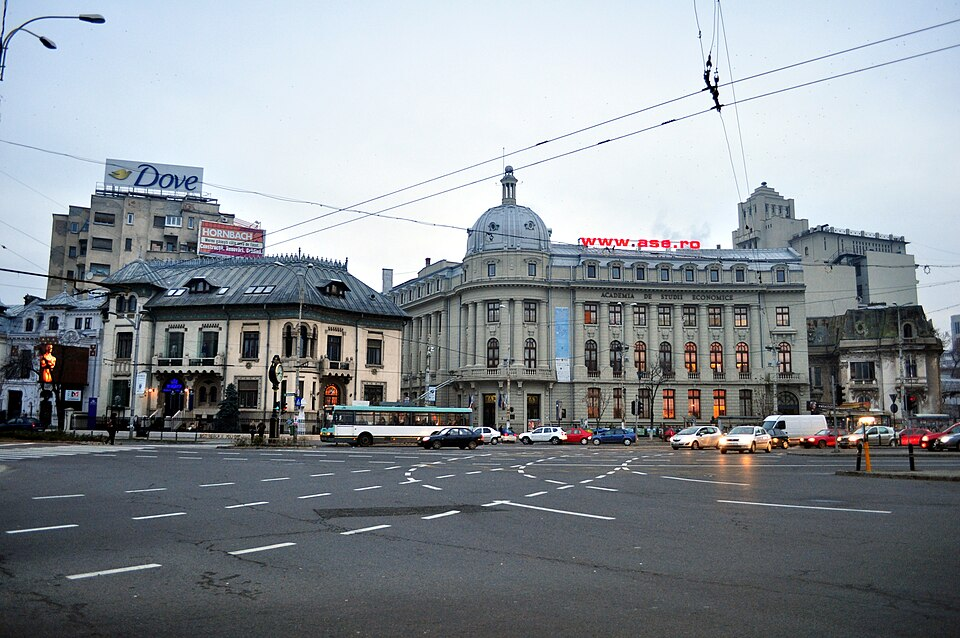
\includegraphics[height=0.46\textheight]{ch0_ase_2014.jpg}\\[1mm]
\imgcap{Academia de Studii Economice din București (ASE)}
\imgcredit{https://commons.wikimedia.org/wiki/File:Bucharest_-_Academie_de_Studii_Economice_01.jpg}{Foto: Joe Mabel (2014); CC BY 3.0; Wikimedia Commons}
\end{column}
\end{columns}
\end{frame}

\begin{frame}{Evaluare}
\itemsize{\small}
\begin{itemize}
    \item \textbf{Examen scris: 70\%}
    \begin{itemize}
        \item citirea și interpretarea rezultatelor obținute în Python, derivări scurte, alegerea modelului potrivit pentru o serie dată
        \item acoperă cursurile și seminariile \tsachlink{https://danpele.github.io/Time-Series-Analysis/RO/Cursuri/capitol0_introducere.pdf}{Capitolelor 0}--\tsachlink{https://danpele.github.io/Time-Series-Analysis/RO/Cursuri/capitol10_spatiul_starilor_kalman_markov_switching.pdf}{10} și \tsachlink{https://danpele.github.io/Time-Series-Analysis/RO/Cursuri/capitol15_recapitulare.pdf}{15}
    \end{itemize}
    \item \textbf{Proiect de echipă: 20\%}
    \begin{itemize}
        \item 2--4 studenți analizează și prognozează serii de timp reale cu metodele cursului
        \item un repository GitHub, un raport scurt, o prezentare și o susținere orală
    \end{itemize}
    \item \textbf{Prezență: 10\%}
    \begin{itemize}
        \item cursuri și seminarii
    \end{itemize}
    \item \textbf{Quiz-uri de autoevaluare}
    \begin{itemize}
        \item cîte unul pentru fiecare capitol, pe site: 20 de întrebări extrase dintr-o bancă de 24, cu explicație pentru fiecare răspuns
    \end{itemize}
\end{itemize}
\end{frame}

\begin{frame}{Manuale}
\itemsize{\small}
\begin{itemize}
    \item \textbf{Manualul de bază}
    \begin{itemize}
        \item \refHP, \emph{Applied Time Series Analysis and Forecasting with Python}, Springer
        \item capitolele cursului urmează ordinea manualului: componente și netezire, staționaritate, ARMA, ARIMA, sezonalitate, volatilitate, modele multivariate
    \end{itemize}
    \item \textbf{Manual însoțitor, gratuit}
    \begin{itemize}
        \item \refFPP, \emph{Forecasting: Principles and Practice} (ediția a 3-a, online)
        \item referința pentru descompunere, netezire exponențială și evaluarea prognozei (\tsachlink{https://danpele.github.io/Time-Series-Analysis/RO/Cursuri/capitol0_introducere.pdf}{Capitolul 0})
    \end{itemize}
    \item \textbf{Teorie}
    \begin{itemize}
        \item \refBD, \emph{Introduction to Time Series and Forecasting}
        \item \refHamilton, \emph{Time Series Analysis}: referința standard a econometriei seriilor de timp
    \end{itemize}
\end{itemize}
\end{frame}

\begin{frame}{Harta cursului: \tsachlinkt{https://danpele.github.io/Time-Series-Analysis/RO/Cursuri/capitol0_introducere.pdf}{Capitolele 0}--\tsachlinkt{https://danpele.github.io/Time-Series-Analysis/RO/Cursuri/capitol15_recapitulare.pdf}{15}}
\itemsize{\footnotesize}
\begin{columns}[T]
\begin{column}{0.49\textwidth}
\begin{center}
\footnotesize
\begin{tabular}{r>{\raggedright\arraybackslash}p{5.6cm}}
\toprule
\textbf{Nr.} & \textbf{Capitol} \\
\midrule
0 & Introducere: componente și netezire exponențială \\
1 & Procese stochastice și staționaritate \\
2 & Modele ARMA \\
3 & Rădăcini unitare și modele ARIMA \\
4 & Sezonalitate și prognoză: SARIMA, TBATS, Prophet \\
5 & Volatilitate condiționată: ARCH și GARCH \\
6 & Modele VAR și cauzalitate Granger \\
7 & Cointegrare și VECM \\
\bottomrule
\end{tabular}
\end{center}

\end{column}
\begin{column}{0.49\textwidth}
\begin{center}
\footnotesize
\begin{tabular}{r>{\raggedright\arraybackslash}p{5.6cm}}
\toprule
\textbf{Nr.} & \textbf{Capitol} \\
\midrule
8 & Memorie lungă și ARFIMA \\
9 & Învățare automată pentru serii de timp \\
10 & Modele în spațiul stărilor, filtrul Kalman și modele Markov switching \\
11 & Foundation models pentru serii de timp$^*$ \\
12 & Analiză spectrală$^*$ \\
13 & Bule speculative: modele LPPL$^*$ \\
14 & Modele GARCH multivariate$^*$ \\
15 & Recapitulare și pregătire pentru examen \\
\bottomrule
\end{tabular}
\end{center}

\end{column}
\end{columns}
\begin{itemize}
    \item Modele univariate (0--5), mai multe serii (6, 7), extensii (8--10), recapitulare (15)
    \item Studiu individual, marcat cu $^*$: \tsachlink{https://danpele.github.io/Time-Series-Analysis/RO/Cursuri/capitol11_foundation_models_serii_timp.pdf}{Capitolele 11}--\tsachlink{https://danpele.github.io/Time-Series-Analysis/RO/Cursuri/capitol14_modele_garch_multivariate.pdf}{14} (materiale mai scurte și un quiz, fără seminar obligatoriu)
\end{itemize}
\end{frame}

\begin{frame}{Materiale și instrumente}
\itemsize{\small}
\begin{itemize}
    \item \textbf{Pentru fiecare capitol}
    \begin{itemize}
        \item slide-urile de curs și de seminar, în română și în engleză
        \item un notebook de curs și unul de seminar (Python), care se deschid în Google Colab cu un singur clic
        \item un quiz de 20 de întrebări
    \end{itemize}
    \item \textbf{Quantlets}: fiecare grafic are un folder public cu codul, un fișier de descriere (\texttt{Metainfo.txt}) și graficul
    \begin{itemize}
        \item pictograma de sub fiecare grafic deschide Quantlet-ul corespunzător pe GitHub
    \end{itemize}
    \item \textbf{Date}: surse publice, citite direct în cod
    \begin{itemize}
        \item Eurostat, INS, BNR, FRED (Federal Reserve Bank of St.\ Louis)
        \item date zilnice de piață de la EODHD (EOD Historical Data), salvate în repository-ul cursului pînă la 18 septembrie 2026
    \end{itemize}
\end{itemize}
\end{frame}

\begin{frame}{Seminarii}
\itemsize{\small}
\begin{itemize}
    \item \textbf{Fiecare seminar are loc înaintea cursului său}
    \begin{itemize}
        \item începe cu noțiunile necesare, deci poate fi urmat fără curs
        \item cursul explică apoi de ce funcționează instrumentele și unde dau greș
    \end{itemize}
    \item \textbf{Trei părți}
    \begin{itemize}
        \item A: calcule scurte pe hîrtie; B: date reale, fiecare cerință încheindu-se cu o întrebare de interpretare; C: o idee deschisă și critica unui răspuns generat de AI
    \end{itemize}
    \item \textbf{Două tipuri de exerciții}
    \begin{itemize}
        \item \textbf{[Rezolvat]}: rezolvarea completă în slide-uri și în notebook, un model de urmat
        \item \textbf{[Propus]}: îl rezolvați dumneavoastră; rezolvarea se discută la seminar
    \end{itemize}
    \item \textbf{Seminarul nu se notează}: are rol de exercițiu pentru examen și pentru proiect
\end{itemize}
\end{frame}

\begin{frame}{Proiectul de echipă}
\itemsize{\small}
\begin{itemize}
    \item \textbf{Întrebarea}: o întrebare de prognoză sau de modelare pe serii de timp reale, aleasă de echipă
    \item \textbf{Metode}: cele din curs
    \begin{itemize}
        \item descompunere și netezire, ARIMA și SARIMA, GARCH, VAR sau VECM, cauzalitate Granger, funcții de răspuns la impuls, evaluarea prognozei
        \item sînt recomandate datele românești (INS, BNR, Eurostat, BVB)
    \end{itemize}
    \item \textbf{Livrabile}
    \begin{itemize}
        \item un repository GitHub al cărui cod reproduce fiecare rezultat numeric și fiecare grafic
        \item un raport scurt, o prezentare și fișierul \texttt{AI\_USE.md}
    \end{itemize}
    \item \textbf{Criterii de evaluare}
    \begin{itemize}
        \item o întrebare clară, metode și diagnosticări corecte, o evaluare onestă în afara eșantionului
        \item \textbf{susținere orală}: fiecare membru explică codul și rezultatele
    \end{itemize}
\end{itemize}
\end{frame}

\begin{frame}{Politica privind AI}
\itemsize{\small}
\begin{itemize}
    \item \textbf{Instrumentele AI sînt permise și trebuie declarate}
    \begin{itemize}
        \item AI (artificial intelligence, inteligență artificială): aici, asistenți construiți pe un LLM (model lingvistic de mari dimensiuni), care scriu text și cod
        \item fiecare utilizare se consemnează în \texttt{AI\_USE.md}: instrumentul, promptul, ce s-a păstrat, ce s-a corectat
    \end{itemize}
    \item \textbf{Răspundeți pentru fiecare rezultat numeric și pentru fiecare referință}
    \begin{itemize}
        \item greșeli tipice ale AI: referințe inventate, formule greșite, cod care rulează, dar calculează altceva
        \item fiecare referință: deschideți DOI-ul (Digital Object Identifier) și verificați titlul
        \item fiecare rezultat numeric: recalculați-l cu propriul cod
    \end{itemize}
    \item \textbf{Susținerea orală}
    \begin{itemize}
        \item o linie de cod pe care nu o puteți explica nu este considerată muncă proprie
    \end{itemize}
\end{itemize}
\end{frame}

\begin{frame}{Recapitulare: organizarea cursului}
\itemsize{\small}
\begin{itemize}
    \item Nota: 70\% examen scris, 20\% proiect de echipă, 10\% prezență
    \item Manual: \refHP; manual însoțitor gratuit: \refFPP
    \item \tsachlink{https://danpele.github.io/Time-Series-Analysis/RO/Cursuri/capitol0_introducere.pdf}{Capitolele 0}--\tsachlink{https://danpele.github.io/Time-Series-Analysis/RO/Cursuri/capitol15_recapitulare.pdf}{15}; \tsachlink{https://danpele.github.io/Time-Series-Analysis/RO/Cursuri/capitol11_foundation_models_serii_timp.pdf}{Capitolele 11}--\tsachlink{https://danpele.github.io/Time-Series-Analysis/RO/Cursuri/capitol14_modele_garch_multivariate.pdf}{14} sînt de studiu individual
    \item Seminariile preced cursurile și nu se notează
    \item AI este permis, declarat în \texttt{AI\_USE.md} și verificat la susținerea orală
\end{itemize}
\end{frame}


%=============================================================================
\section{Seria de timp}
%=============================================================================

\begin{frame}{Definiție}
\itemsize{\small}
\begin{itemize}
    \item \textbf{Serie de timp}: observații ale unei variabile, înregistrate în momente succesive și ordonate în timp
    \item \textbf{Notație}: $y_1, y_2, \ldots, y_T$
    \begin{itemize}
        \item $t$: indicele de timp (trimestru, lună, zi); $T$: numărul de observații
        \item \textbf{frecvența}: numărul de observații pe an (4 trimestriale, 12 lunare, aproximativ 252 pentru zilele de tranzacționare)
    \end{itemize}
    \item \textbf{Exemplu}: PIB-ul real al României, trimestrial, miliarde EUR în prețurile anului 2010
    \begin{itemize}
        \item T1 2024: 38{,}7; T2 2024: 45{,}6; T3 2024: 52{,}8; T4 2024: 59{,}2; T1 2025: 38{,}9
        \item ordinea contează: dacă amestecăm cele cinci valori, pierdem informația
    \end{itemize}
    \item PIB: produsul intern brut; T1--T4: cele patru trimestre ale unui an
\end{itemize}
\end{frame}

\begin{frame}{Trei tipuri de date}
\itemsize{\footnotesize}
\begin{center}
\footnotesize
\begin{tabular}{>{\raggedright\arraybackslash}p{2.6cm}>{\raggedright\arraybackslash}p{4.2cm}>{\raggedright\arraybackslash}p{5.4cm}}
\toprule
\textbf{Tip} & \textbf{Structură} & \textbf{Exemplu} \\
\midrule
Date transversale & multe unități, un singur moment & PIB-ul celor 27 de țări UE în 2025 \\
Serie de timp & o unitate, multe momente & PIB-ul României, în fiecare trimestru din 1995 \\
Date panel & multe unități, multe momente & PIB-ul celor 27 de țări UE, în fiecare trimestru \\
\bottomrule
\end{tabular}
\end{center}
\begin{itemize}
    \item \textbf{Particularitatea seriilor de timp}
    \begin{itemize}
        \item observațiile \textbf{nu sînt independente}: trimestrul acesta seamănă cu cel anterior
        \item această dependență este chiar informația pe care o folosim pentru prognoză
        \item formulele clasice pentru eșantioane independente (erori standard, teste) trebuie adaptate
    \end{itemize}
    \item UE: Uniunea Europeană
\end{itemize}
\end{frame}

\begin{frame}{Importanța seriilor de timp}
\itemsize{\footnotesize}
\begin{center}
\footnotesize
\begin{tabular}{>{\raggedright\arraybackslash}p{1.9cm}>{\raggedright\arraybackslash}p{4.3cm}>{\raggedright\arraybackslash}p{6.2cm}}
\toprule
\textbf{Domeniu} & \textbf{Serie} & \textbf{Întrebare tipică} \\
\midrule
Economie & PIB, inflație, șomaj & Unde va fi inflația peste un an? \\
Finanțe & cursuri de schimb, indici bursieri, dobînzi & Cît de riscant este BET mîine? \\
Energie & producția și consumul de electricitate, prețuri & De cîtă electricitate este nevoie în ianuarie viitor? \\
Climă & concentrația de CO2, temperaturi & Cît de repede crește CO2, dincolo de oscilația sezonieră? \\
\bottomrule
\end{tabular}
\end{center}
\begin{itemize}
    \item Deciziile depind de prognoze: banca centrală stabilește dobînda pe baza prognozei inflației; operatorul de rețea planifică producția pe baza prognozei cererii
\end{itemize}
\end{frame}

\begin{frame}{Patru obiective ale analizei seriilor de timp}
\itemsize{\small}
\begin{itemize}
    \item \textbf{Descriere}: trend, sezonalitate, cicluri, observații neobișnuite
    \begin{itemize}
        \item grafice, descompunere, autocorelație (acest capitol și \tsachlink{https://danpele.github.io/Time-Series-Analysis/RO/Cursuri/capitol1_procese_stochastice_stationaritate.pdf}{Capitolul 1})
    \end{itemize}
    \item \textbf{Modelare}: un model probabilist care ar fi putut genera datele
    \begin{itemize}
        \item ARMA, ARIMA, GARCH (\tsachlink{https://danpele.github.io/Time-Series-Analysis/RO/Cursuri/capitol2_modele_arma.pdf}{Capitolele 2}--\tsachlink{https://danpele.github.io/Time-Series-Analysis/RO/Cursuri/capitol5_volatilitate_conditionata_garch.pdf}{5})
    \end{itemize}
    \item \textbf{Prognoză}: valori încă neobservate, împreună cu incertitudinea lor
    \begin{itemize}
        \item obiectivul care străbate întregul curs
    \end{itemize}
    \item \textbf{Explicare și control}: cum răspunde o serie la modificarea alteia
    \begin{itemize}
        \item modele VAR, cauzalitate Granger, cointegrare (\tsachlink{https://danpele.github.io/Time-Series-Analysis/RO/Cursuri/capitol6_modele_var_cauzalitate_granger.pdf}{Capitolele 6} și \tsachlink{https://danpele.github.io/Time-Series-Analysis/RO/Cursuri/capitol7_cointegrare_vecm.pdf}{7})
    \end{itemize}
    \item \refBJ\ au formulat aceleași obiective: identificare, estimare, verificare, prognoză
\end{itemize}
\end{frame}

\begin{frame}{Frecvență, fluxuri și stocuri, date ajustate}
\itemsize{\small}
\begin{itemize}
    \item \textbf{Flux}: măsurat pe o perioadă; \textbf{stoc}: măsurat la un moment
    \begin{itemize}
        \item fluxuri: PIB-ul unui trimestru, electricitatea produsă într-o lună; se adună în timp
        \item stocuri: cursul de schimb dintr-o zi, concentrația de CO2, nivelul unui indice; le mediem, nu le adunăm
    \end{itemize}
    \item \textbf{Schimbarea frecvenței}
    \begin{itemize}
        \item din lunar în trimestrial: suma pentru fluxuri, media sau ultima valoare pentru stocuri
    \end{itemize}
    \item \textbf{Date ajustate sezonier}
    \begin{itemize}
        \item institutul de statistică elimină tiparul regulat din interiorul anului și efectele de calendar (numărul de zile lucrătoare)
        \item seria neajustată este cea măsurată; seria ajustată este o estimare, revizuită cînd apar date noi
    \end{itemize}
\end{itemize}
\end{frame}

\begin{frame}{Datele folosite în acest capitol}
\itemsize{\footnotesize}
\begin{center}
\footnotesize
\begin{tabular}{>{\raggedright\arraybackslash}p{4.0cm}>{\raggedright\arraybackslash}p{3.0cm}>{\raggedright\arraybackslash}p{2.6cm}>{\raggedright\arraybackslash}p{2.8cm}}
\toprule
\textbf{Serie} & \textbf{Sursă} & \textbf{Frecvență} & \textbf{Eșantion} \\
\midrule
PIB-ul real al României & Eurostat & trimestrial & T1 1995 -- T2 2026 \\
IAPC, prețurile de consum & Eurostat & lunar & 1996 -- august 2026 \\
Producția de electricitate, România & Eurostat & lunar & ianuarie 2008 -- iulie 2026 \\
EUR/RON & cursul de referință BNR & zilnic & 2005 -- 2026 \\
BET, S\&P 500 & EODHD & zilnic & 2000 -- 2026 \\
CO2 la Mauna Loa & setul de date statsmodels & săptămînal, mediat lunar & 1958 -- 2001 \\
\bottomrule
\end{tabular}
\end{center}
\begin{itemize}
    \item IAPC: indicele armonizat al prețurilor de consum (HICP, Harmonised Index of Consumer Prices), calculat cu aceeași metodă în toate țările UE
    \item BET: indicele de referință al BVB; S\&P 500: 500 de companii mari din SUA
    \item statsmodels: biblioteca Python de modele statistice folosită pe tot parcursul cursului
\end{itemize}
\end{frame}

\begin{frame}{Recapitulare: seria de timp}
\itemsize{\small}
\begin{itemize}
    \item O serie de timp este o variabilă observată în timp; ordinea observațiilor conține informație
    \item Observațiile consecutive depind unele de altele: pe acest fapt se sprijină prognoza
    \item Obiective: descriere, modelare, prognoză, explicare
    \item Fluxurile se adună, stocurile se mediază; seriile ajustate sînt estimări
\end{itemize}
\end{frame}


%=============================================================================
\section{Serii de timp pe date reale}
%=============================================================================

\begin{frame}{PIB-ul real al României}
\itemsize{\footnotesize}
\begin{center}
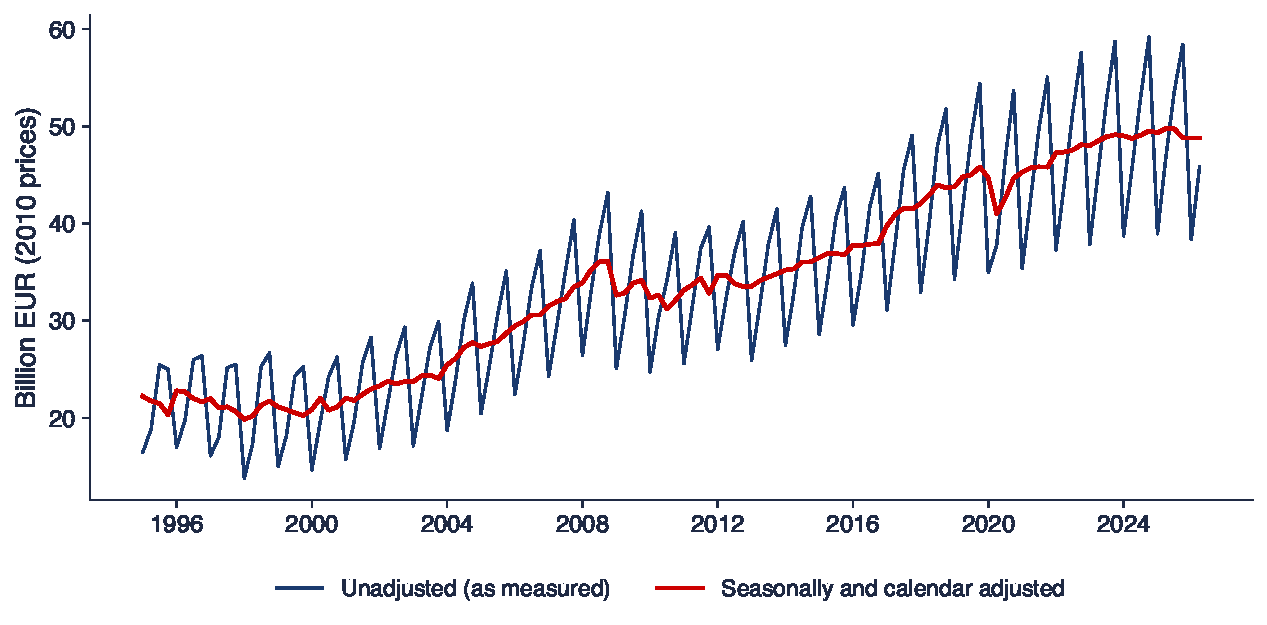
\includegraphics[width=0.94\textwidth,height=0.6\textheight,keepaspectratio]{tsa_ch0_gdp.pdf}
\end{center}
\vspace{-2mm}
\begin{itemize}
    \item Trimestrial, T1 1995 -- T2 2026, volume înlănțuite în prețurile anului 2010 (miliarde EUR); albastru: seria măsurată; roșu: seria ajustată sezonier și cu efectele de calendar (Eurostat)
\end{itemize}
\quantlet{TSA\_ch0\_examples}{\qlurl{TSA_ch0_examples}}
\end{frame}

\begin{frame}{Interpretarea: PIB}
\itemsize{\small}
\begin{itemize}
    \item \textbf{Trend}: economia a crescut de aproximativ 2{,}3 ori din 1995 pînă în 2025
    \begin{itemize}
        \item o creștere reală medie de 2{,}8\% pe an
    \end{itemize}
    \item \textbf{Sezonalitate}: în fiecare an, trimestrul I este mult sub trimestrul IV
    \begin{itemize}
        \item iarna: mai puține construcții și lucrări agricole; toamna: recolta și activitatea de la sfîrșit de an
        \item oscilația crește odată cu nivelul PIB: un tipar multiplicativ
    \end{itemize}
    \item \textbf{Ciclu}: recesiunile întrerup trendul
    \begin{itemize}
        \item PIB-ul anual a scăzut cu 5{,}5\% în 2009 (criza financiară globală) și cu 3{,}6\% în 2020 (pandemia de COVID-19)
    \end{itemize}
    \item Ultima valoare, T2 2026: 45{,}9 miliarde EUR neajustat, 48{,}8 ajustat
\end{itemize}
\end{frame}

\begin{frame}{Prețurile de consum și inflația în România}
\itemsize{\footnotesize}
\begin{center}
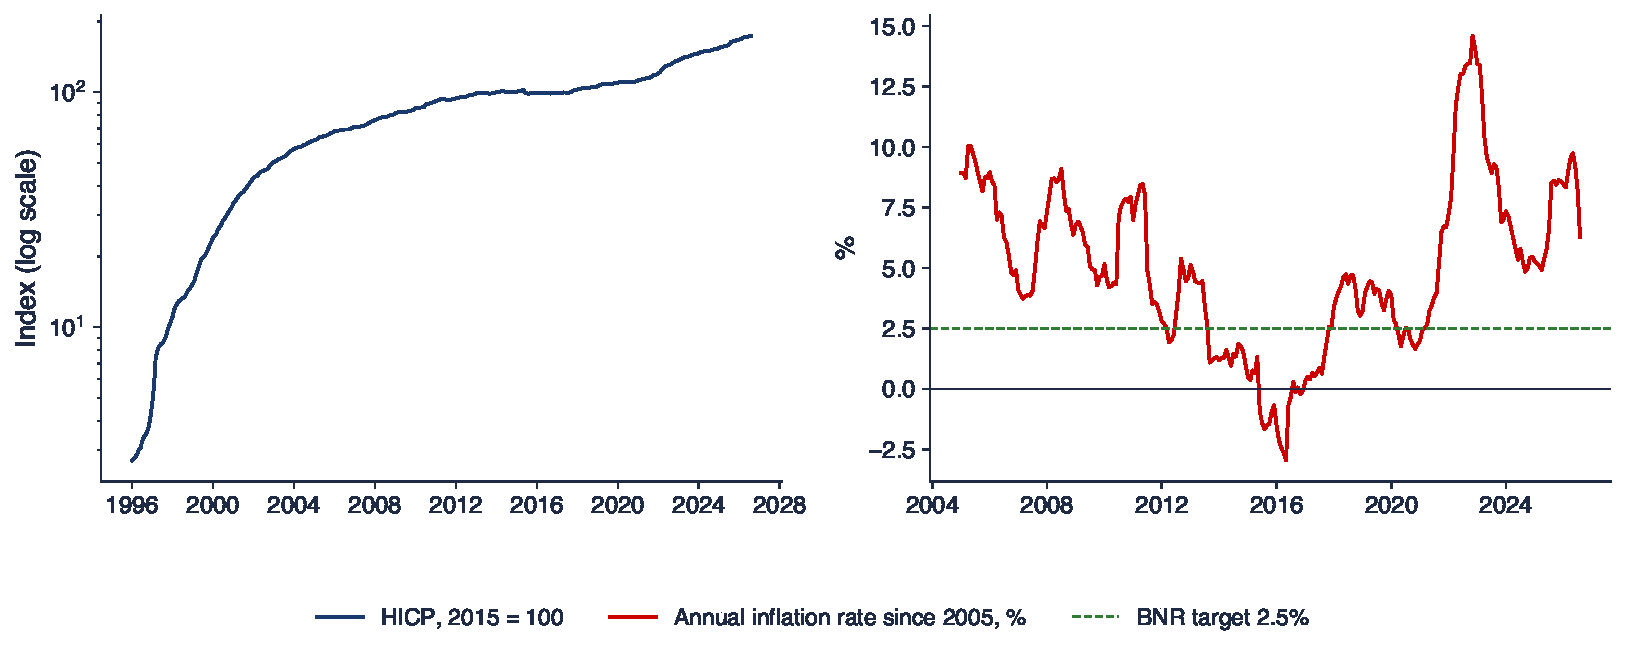
\includegraphics[width=0.94\textwidth,height=0.58\textheight,keepaspectratio]{tsa_ch0_hicp.pdf}
\end{center}
\vspace{-2mm}
\begin{itemize}
    \item Stînga: IAPC, 2015 = 100, scară logaritmică; dreapta: rata anuală a inflației $100\,(P_t/P_{t-12} - 1)$ din 2005, față de ținta BNR de 2,5\%; $P_t$: IAPC în luna $t$
\end{itemize}
\quantlet{TSA\_ch0\_examples}{\qlurl{TSA_ch0_examples}}
\end{frame}

\begin{frame}{Interpretarea: inflația}
\itemsize{\small}
\begin{itemize}
    \item \textbf{Nivelul și rata oferă informații diferite}
    \begin{itemize}
        \item indicele prețurilor aproape nu scade niciodată: trendul lui este inflația acumulată
        \item rata inflației crește și scade: este seria pe care o țintește banca centrală
    \end{itemize}
    \item \textbf{Episoade}
    \begin{itemize}
        \item iunie 1997: 178\%, după liberalizarea prețurilor din 1997
        \item mai 2016: \ensuremath{-}3{,}0\%, după reducerile de TVA din 2015--2016
        \item noiembrie 2022: 14{,}6\%, șocul prețurilor la energie
        \item august 2026: 6{,}3\%
    \end{itemize}
    \item O rată calculată pe 12 luni elimină tiparul sezonier, dar reacționează cu întîrziere: reflectă întregul an trecut
    \item TVA: taxa pe valoarea adăugată
\end{itemize}
\end{frame}

\begin{frame}{EUR/RON, cursul de referință BNR}
\itemsize{\footnotesize}
\begin{center}
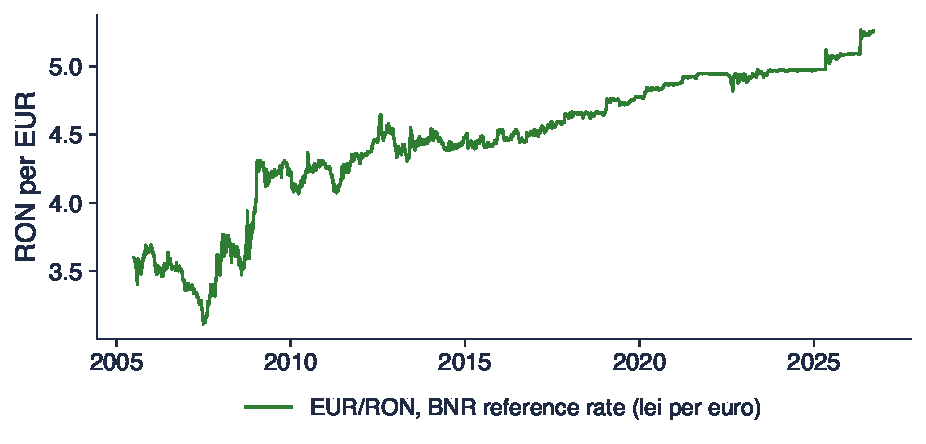
\includegraphics[width=0.94\textwidth,height=0.6\textheight,keepaspectratio]{tsa_ch0_eurron.pdf}
\end{center}
\vspace{-2mm}
\begin{itemize}
    \item Lei pentru un euro, în fiecare zi lucrătoare de la 4 iulie 2005 la 18 septembrie 2026 (5\,353 de observații)
\end{itemize}
\quantlet{TSA\_ch0\_examples}{\qlurl{TSA_ch0_examples}}
\end{frame}

\begin{frame}{Interpretarea: EUR/RON}
\itemsize{\small}
\begin{itemize}
    \item \textbf{Un trend fără o formă fixă}
    \begin{itemize}
        \item de la 3{,}5986 la 5{,}2644 lei; valoarea minimă 3{,}1112 pe 2 iulie 2007
        \item perioade lungi de calm, întrerupte de salturi (toamna lui 2008, 2012, 2025)
    \end{itemize}
    \item \textbf{Fără sezonalitate}
    \begin{itemize}
        \item dacă euro ar fi, previzibil, mai ieftin în fiecare primăvară, participanții la piață l-ar cumpăra primăvara și tiparul ar dispărea
    \end{itemize}
    \item \textbf{Variațiile zilnice}
    \begin{itemize}
        \item abaterea standard a variației logaritmice zilnice: 0{,}28\%; cea mai mare variație: 2{,}93\% pe 3 octombrie 2008
    \end{itemize}
    \item Un astfel de trend, format din șocuri acumulate, se numește \textbf{trend stochastic} (\tsachlink{https://danpele.github.io/Time-Series-Analysis/RO/Cursuri/capitol1_procese_stochastice_stationaritate.pdf}{Capitolele 1} și \tsachlink{https://danpele.github.io/Time-Series-Analysis/RO/Cursuri/capitol3_radacini_unitare_modele_arima.pdf}{3})
\end{itemize}
\end{frame}

\begin{frame}{BET și S\&P 500 din 2000}
\itemsize{\footnotesize}
\begin{center}
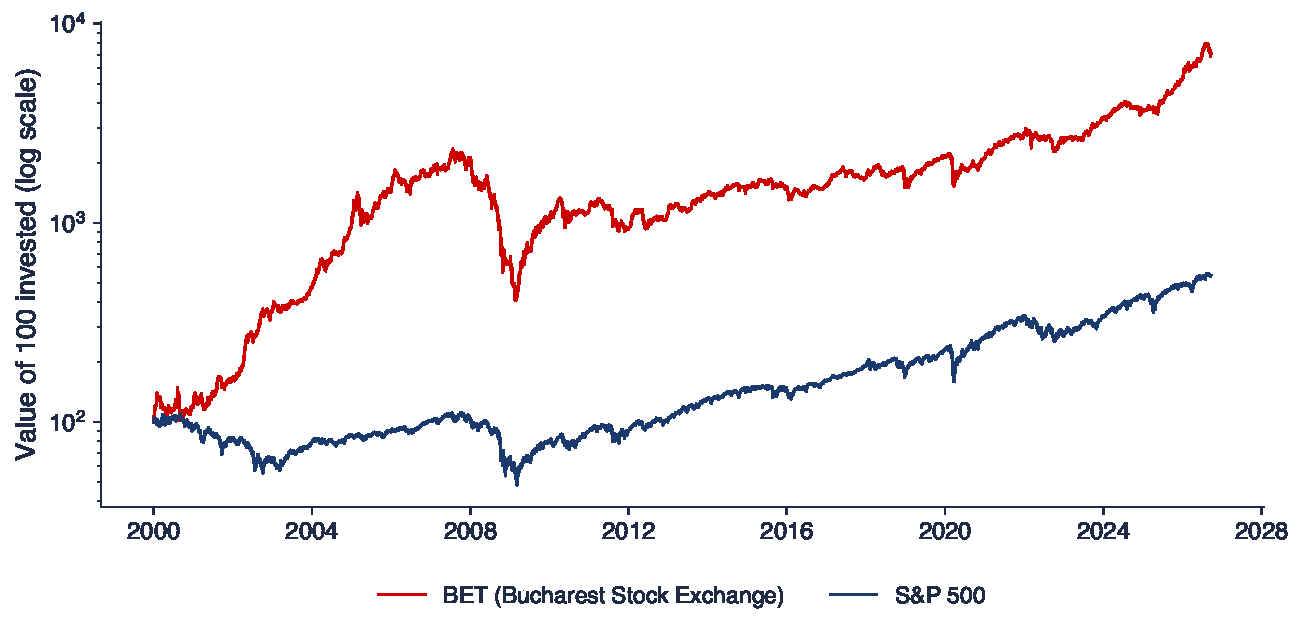
\includegraphics[width=0.94\textwidth,height=0.6\textheight,keepaspectratio]{tsa_ch0_markets.pdf}
\end{center}
\vspace{-2mm}
\begin{itemize}
    \item Valoarea a 100 de unități investite pe 5 ianuarie 2000, prețuri de închidere, scară logaritmică: distanțele verticale egale sînt modificări procentuale egale
\end{itemize}
\quantlet{TSA\_ch0\_examples}{\qlurl{TSA_ch0_examples}}
\end{frame}

\begin{frame}{Interpretarea: indicii bursieri}
\itemsize{\small}
\begin{itemize}
    \item \textbf{Creștere pe termen lung, cu scăderi adînci}
    \begin{itemize}
        \item 100 de unități investite s-au înmulțit de aproximativ 71 de ori în BET și de 5{,}5 ori în S\&P 500 (indici de preț, fără dividende)
        \item 2008--2009: BET a pierdut mai mult de trei sferturi din valoare; revenirea a durat ani
    \end{itemize}
    \item \textbf{Rolul scării logaritmice}
    \begin{itemize}
        \item pe o scară liniară, primii ani par plați, iar variațiile recente par uriașe
        \item logaritmul transformă o creștere procentuală constantă într-o dreaptă
    \end{itemize}
    \item Prețurile activelor tranzacționate se prognozează greu; \textbf{riscul} lor se prognozează mai ușor (\tsachlink{https://danpele.github.io/Time-Series-Analysis/RO/Cursuri/capitol5_volatilitate_conditionata_garch.pdf}{Capitolul 5})
\end{itemize}
\end{frame}

\begin{frame}{Producția de electricitate în România}
\itemsize{\footnotesize}
\begin{center}
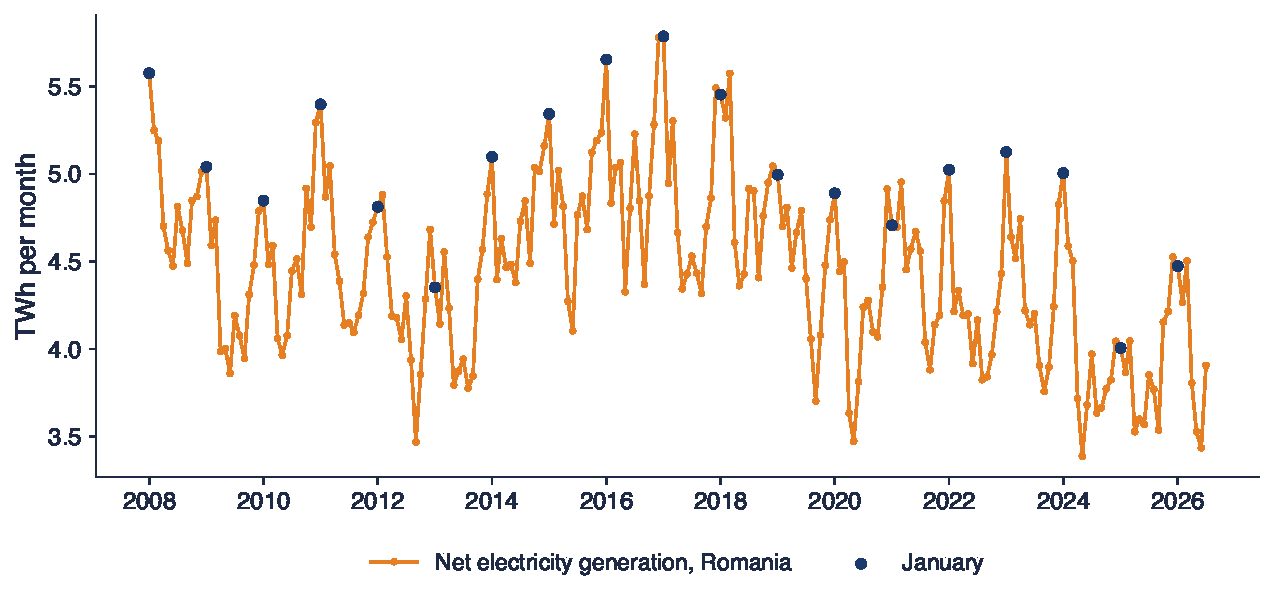
\includegraphics[width=0.94\textwidth,height=0.58\textheight,keepaspectratio]{tsa_ch0_electricity.pdf}
\end{center}
\vspace{-2mm}
\begin{itemize}
    \item Producția netă de electricitate, TWh pe lună, ianuarie 2008 -- iulie 2026 (Eurostat); puncte: luna ianuarie a fiecărui an
\end{itemize}
\quantlet{TSA\_ch0\_examples}{\qlurl{TSA_ch0_examples}}
\end{frame}

\begin{frame}{Interpretarea: electricitatea}
\itemsize{\small}
\begin{itemize}
    \item \textbf{Sezonalitate puternică}
    \begin{itemize}
        \item luna cu media cea mai mare: ianuarie (5{,}03 TWh); cea mai mică: septembrie (4{,}06 TWh)
        \item cererea de iarnă pentru încălzire și iluminat; raportul celor două medii este 1{,}24
    \end{itemize}
    \item \textbf{Un nivel în scădere}
    \begin{itemize}
        \item 58{,}5 TWh în 2008, 46{,}7 TWh în 2025: mai multe importuri, o cerere industrială mai mică
    \end{itemize}
    \item \textbf{Ani atipici}
    \begin{itemize}
        \item anii secetoși reduc producția hidro; iernile blînde reduc cererea
    \end{itemize}
    \item TWh: terawatt-oră, $10^{12}$ wați-oră; GWh: gigawatt-oră, $10^{9}$ wați-oră
\end{itemize}
\end{frame}

\begin{frame}{Curba Keeling}
\itemsize{\footnotesize}
\begin{columns}[T]
\begin{column}{0.6\textwidth}
\begin{itemize}
    \item \textbf{1958}: Charles David Keeling începe măsurarea CO2 la Mauna Loa, Hawaii, departe de surse locale (\refKeeling)
    \begin{itemize}
        \item cea mai lungă serie continuă de măsurători ale CO2 din atmosferă
    \end{itemize}
    \item \textbf{Două tipare într-o singură serie}
    \begin{itemize}
        \item un trend crescător: emisiile din combustibili fosili se acumulează
        \item o undă anuală: plantele din emisfera nordică absorb CO2 vara și îl eliberează iarna
    \end{itemize}
    \item ppm (parts per million): molecule de CO2 la un milion de molecule de aer uscat
    \item CO2: dioxid de carbon
\end{itemize}
\end{column}
\begin{column}{0.36\textwidth}
\centering

\includegraphics[height=0.5\textheight]{ch0_keeling_2001.jpg}\\[1mm]
\imgcap{Charles David Keeling (1928--2005), 2001}
\imgcredit{https://commons.wikimedia.org/wiki/File:Charles_David_Keeling_2001.jpg}{Foto: National Science Foundation (2001); domeniu public; Wikimedia Commons}
\end{column}
\end{columns}
\end{frame}

\begin{frame}{CO2 atmosferic la Mauna Loa}
\itemsize{\footnotesize}
\begin{center}
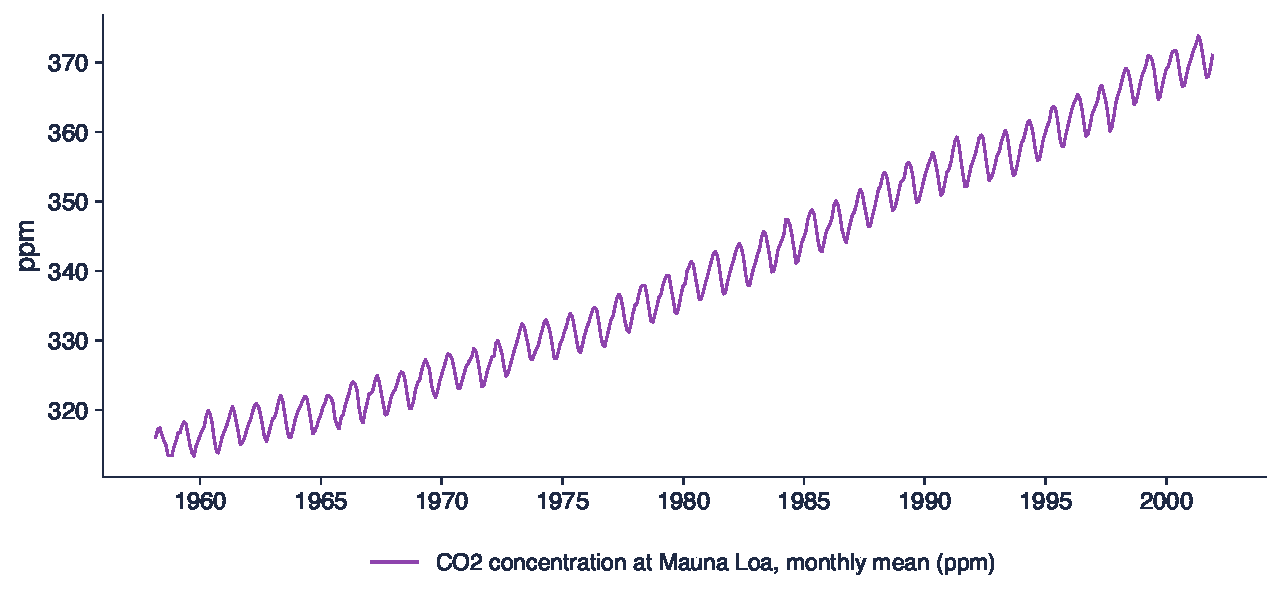
\includegraphics[width=0.94\textwidth,height=0.58\textheight,keepaspectratio]{tsa_ch0_co2.pdf}
\end{center}
\vspace{-2mm}
\begin{itemize}
    \item Mediile lunare ale măsurătorilor săptămînale, martie 1958 -- decembrie 2001 (526 de luni; setul de date clasic din statsmodels)
\end{itemize}
\quantlet{TSA\_ch0\_examples}{\qlurl{TSA_ch0_examples}}
\end{frame}

\begin{frame}{Interpretarea: CO2}
\itemsize{\small}
\begin{itemize}
    \item \textbf{Trend}: de la 316{,}1 la 371{,}0 ppm
    \begin{itemize}
        \item în medie 1{,}26 ppm pe an; panta însăși crește în timp
    \end{itemize}
    \item \textbf{Sezonalitate}: o undă anuală regulată, de cîțiva ppm
    \begin{itemize}
        \item unda își păstrează aproximativ mărimea în timp ce nivelul crește: un tipar aditiv
    \end{itemize}
    \item \textbf{Aproape fără zgomot}
    \begin{itemize}
        \item o măsurătoare fizică atentă, spre deosebire de PIB sau de cursul de schimb
    \end{itemize}
    \item O serie netedă, cu trend și sezonalitate clare: cazul cel mai simplu pentru descompunere și netezire
\end{itemize}
\end{frame}

\begin{frame}{Tipare în șase serii}
\itemsize{\footnotesize}
\begin{center}
\scriptsize
\begin{tabular}{lllll}
\toprule
\textbf{Serie} & \textbf{Trend} & \textbf{Sezonalitate} & \textbf{Ciclu} & \textbf{Zgomot} \\
\midrule
PIB (neajustat) & crescător & puternică, multiplicativă & recesiuni & mic \\
Rata inflației & descrescător după 1997 & eliminată de rata pe 12 luni & șocuri & mediu \\
EUR/RON & stochastic & -- & -- & mediu \\
BET & crescător, cu prăbușiri & -- & avînturi și prăbușiri & mare \\
Electricitate & descrescător & puternică, vîrf iarna & -- & mediu \\
CO2 & crescător, accelerat & regulată, aditivă & -- & foarte mic \\
\bottomrule
\end{tabular}
\end{center}
\begin{itemize}
    \item \textbf{Întrebare pentru sală}: care dintre aceste serii ați prognoza-o cel mai precis cu un an înainte?
    \pause
    \item \textbf{Răspuns}: CO2: un trend neted și o sezonalitate stabilă, puțin zgomot; BET este cea mai grea: fără sezonalitate și cu zgomot mare
\end{itemize}
\end{frame}

\begin{frame}{Recapitulare: serii de timp pe date reale}
\itemsize{\small}
\begin{itemize}
    \item PIB și electricitate: trend și un tipar sezonier puternic; PIB arată și recesiunile
    \item Inflația: rata pe 12 luni elimină sezonalitatea, dar reacționează tîrziu
    \item EUR/RON și BET: trenduri formate din șocuri, fără sezonalitate, greu de prognozat
    \item CO2: un trend neted și o undă anuală aditivă
    \item Priviți întîi graficul: el orientează alegerea modelului
\end{itemize}
\end{frame}


%=============================================================================
\section{O scurtă istorie}
%=============================================================================

\begin{frame}{Petele solare: prima serie de timp celebră}
\itemsize{\footnotesize}
\begin{columns}[T]
\begin{column}{0.30\textwidth}
\centering
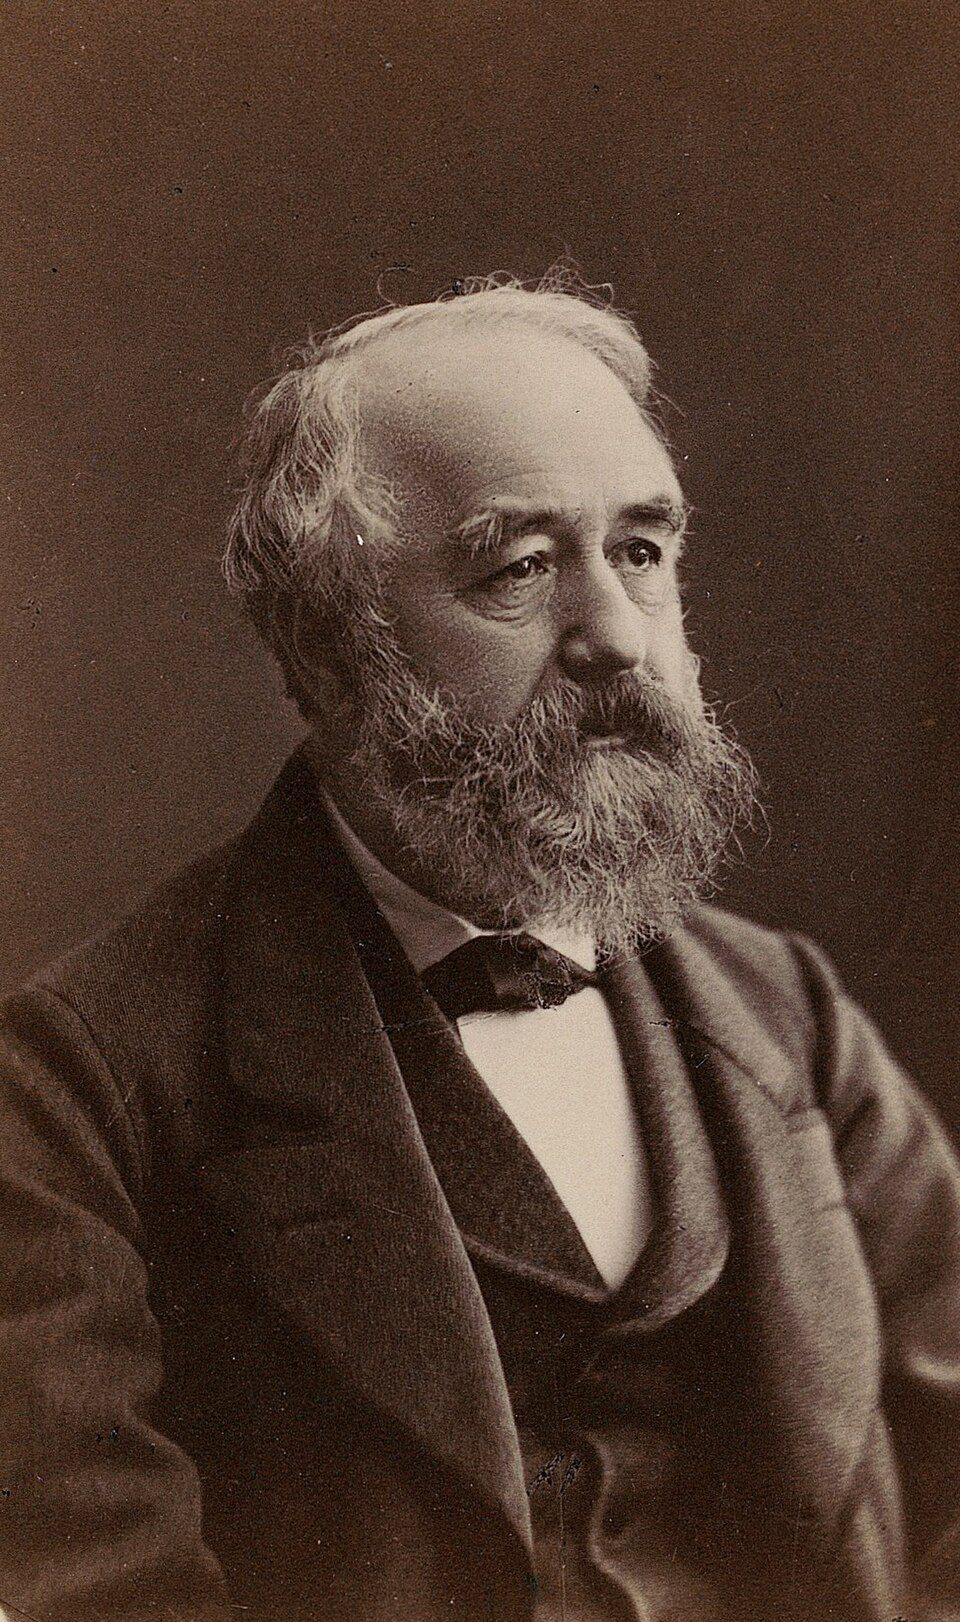
\includegraphics[height=0.42\textheight]{ch0_wolf.jpg}\\[1mm]
\imgcap{Rudolf Wolf (1816--1893)}
\imgcredit{https://commons.wikimedia.org/wiki/File:ETH-BIB-Wolf,_Johann_Rudolf_(1816-1893)-Portrait-Portr_12033-RE.tif_(cropped).jpg}{Foto: Emil Gassler (1888--1893); domeniu public; ETH-Bibliothek, Wikimedia Commons}
\end{column}
\begin{column}{0.66\textwidth}
\begin{itemize}
    \item \textbf{1848}: astronomul elvețian Rudolf Wolf definește un indice zilnic al activității solare, pe baza numărului de pete solare
    \item îl reconstituie pînă în 1749: numerele de pete solare Wolf (ulterior Wolfer)
    \item seria crește și scade în valuri de aproximativ 11 ani, dar nici lungimea, nici înălțimea valurilor nu sînt constante
    \item întrebarea: un semnal periodic ascuns, peste care se suprapune zgomot, sau altceva?
\end{itemize}
\centering
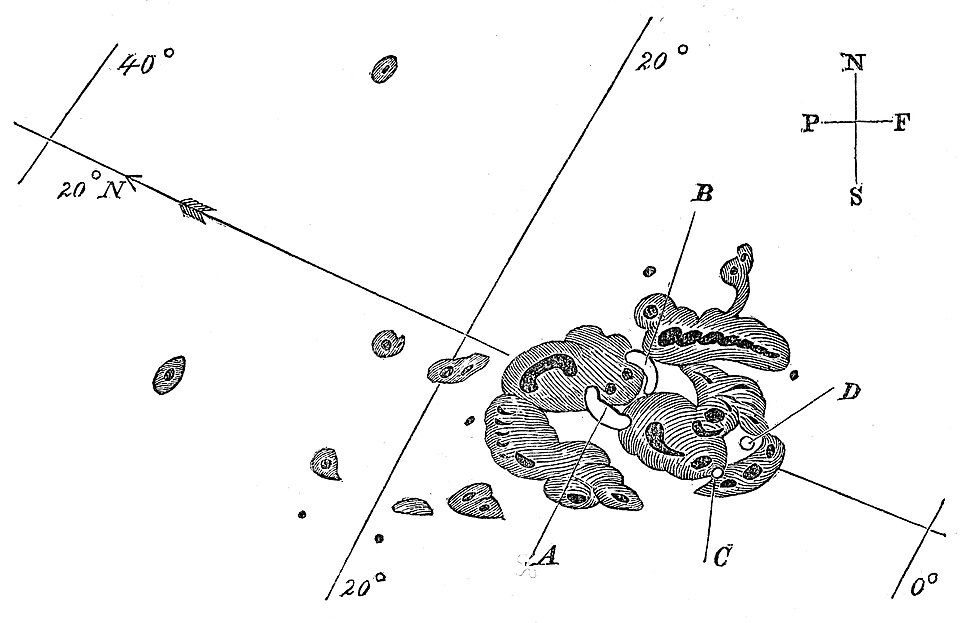
\includegraphics[height=0.26\textheight]{ch0_sunspots_1859.jpg}\\[1mm]
\imgcap{Pete solare desenate de Richard Carrington, 1 septembrie 1859}
\imgcredit{https://commons.wikimedia.org/wiki/File:Carrington_Richard_drawing_of_1859_sunspots.jpeg}{Desen: Richard Carrington (1859); domeniu public; Wikimedia Commons}
\end{column}
\end{columns}
\end{frame}

\begin{frame}{Yule (1926, 1927): dependența este modelul}
\itemsize{\small}
\begin{itemize}
    \item \textbf{1926}: \emph{corelațiile fără sens} dintre seriile de timp (\refYuleNonsense)
    \begin{itemize}
        \item două serii fără nicio legătură, dar cu trend, pot avea o corelație apropiată de 1
        \item exemplul lui: ponderea căsătoriilor oficiate de Biserica Angliei și rata mortalității în Anglia și Țara Galilor
        \item astăzi: regresia falsă (\tsachlink{https://danpele.github.io/Time-Series-Analysis/RO/Cursuri/capitol3_radacini_unitare_modele_arima.pdf}{Capitolul 3}) și cointegrarea (\tsachlink{https://danpele.github.io/Time-Series-Analysis/RO/Cursuri/capitol7_cointegrare_vecm.pdf}{Capitolul 7})
    \end{itemize}
    \item \textbf{1927}: numerele lui Wolfer explicate prin propriul trecut (\refYule)
    \begin{itemize}
        \item în locul unor sinusoide ascunse: $y_t = \phi_1 y_{t-1} + \phi_2 y_{t-2} + \varepsilon_t$, cu perturbații aleatoare $\varepsilon_t$
        \item $y_t$: numărul de pete solare din anul $t$; $\phi_1, \phi_2$: coeficienți estimați din date, care fixează lungimea și amortizarea valurilor
        \item primul model \textbf{autoregresiv}: AR(2) (\tsachlink{https://danpele.github.io/Time-Series-Analysis/RO/Cursuri/capitol2_modele_arma.pdf}{Capitolul 2})
        \item perturbațiile deplasează valurile, deci perioada variază, ca în date
    \end{itemize}
\end{itemize}
\end{frame}

\begin{frame}{Slutsky (1937): cicluri din șocuri aleatoare}
\itemsize{\footnotesize}
\begin{columns}[T]
\begin{column}{0.28\textwidth}
\centering
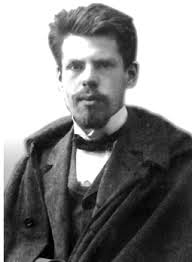
\includegraphics[height=0.42\textheight]{ch0_slutsky.jpg}\\[1mm]
\imgcap{Eugen Slutsky (1880--1948)}
\imgcredit{https://commons.wikimedia.org/wiki/File:\%D0\%A1\%D0\%BB\%D1\%83\%D1\%86\%D1\%8C\%D0\%BA\%D0\%B8\%D0\%B9_\%D0\%84\%D0\%B2\%D0\%B3\%D0\%B5\%D0\%BD.jpg}{Foto: autor necunoscut; domeniu public; Wikimedia Commons}
\end{column}
\begin{column}{0.68\textwidth}
\begin{itemize}
    \item \textbf{1927} (Moscova), \textbf{1937} în engleză: \emph{Însumarea cauzelor aleatoare ca sursă a proceselor ciclice} (\refSlutsky)
    \item \textbf{Experimentul}
    \begin{itemize}
        \item se iau numere aleatoare independente $\varepsilon_1, \varepsilon_2, \ldots$ (cifrele unei extrageri la loterie)
        \item fiecare număr se înlocuiește cu suma ultimelor 10: $y_t = \varepsilon_t + \varepsilon_{t-1} + \cdots + \varepsilon_{t-9}$
        \item rezultatul seamănă cu ciclurile economice
    \end{itemize}
    \item Astăzi, acesta este un proces de \textbf{medie mobilă}: MA(9) (\tsachlink{https://danpele.github.io/Time-Series-Analysis/RO/Cursuri/capitol2_modele_arma.pdf}{Capitolul 2})
\end{itemize}
\end{column}
\end{columns}
\end{frame}

\begin{frame}{Experimentul lui Slutsky, simulat}
\itemsize{\footnotesize}
\begin{center}
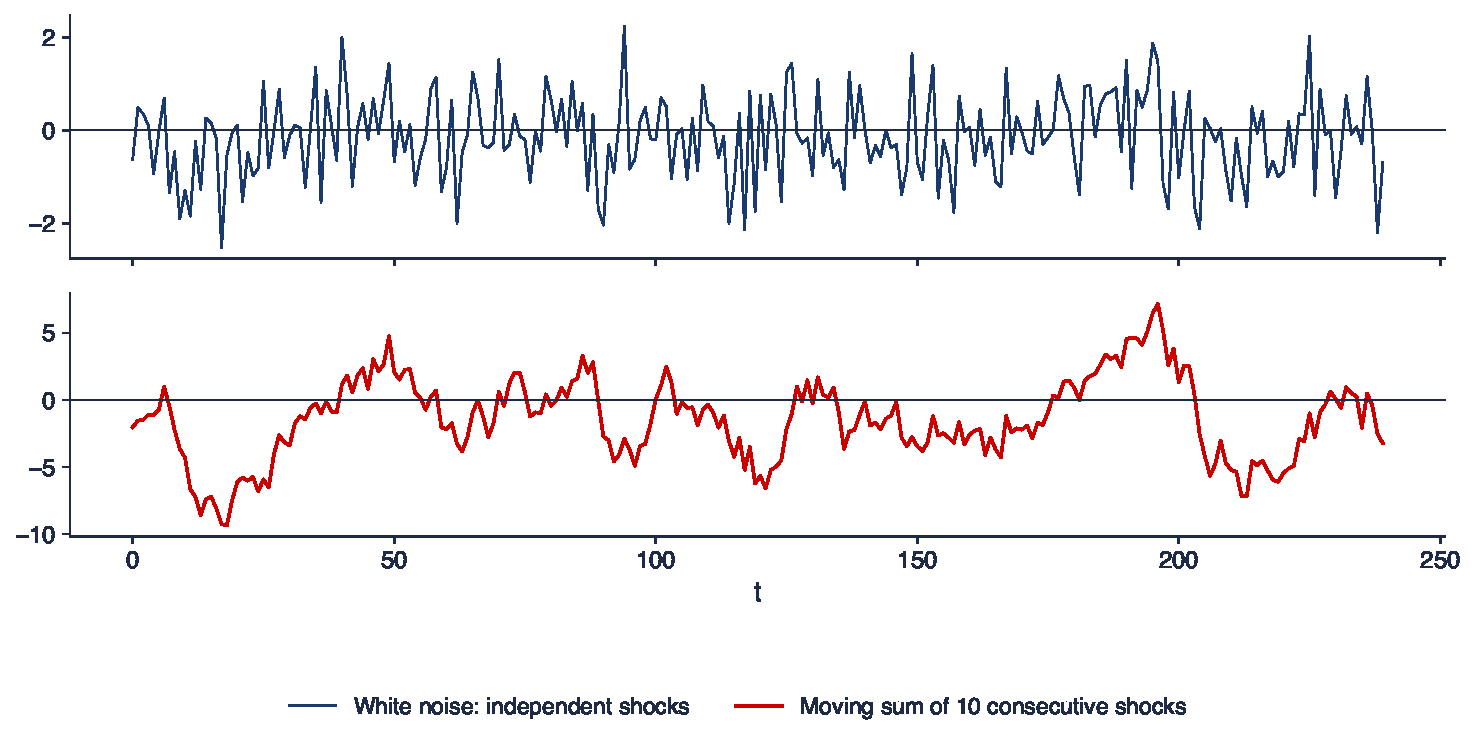
\includegraphics[width=0.94\textwidth,height=0.58\textheight,keepaspectratio]{tsa_ch0_slutsky.pdf}
\end{center}
\vspace{-2mm}
\begin{itemize}
    \item Sus: 240 de șocuri independente, cu distribuția Normală standard; jos: suma mobilă a cîte 10 șocuri consecutive
\end{itemize}
\quantlet{TSA\_ch0\_slutsky}{\qlurl{TSA_ch0_slutsky}}
\end{frame}

\begin{frame}{Interpretarea: experimentul lui Slutsky}
\itemsize{\small}
\begin{itemize}
    \item \textbf{Nu am introdus niciun ciclu, totuși apar valuri}
    \begin{itemize}
        \item suma mobilă traversează zero în sus de 16 ori în 240 de perioade: valuri de lungime neregulată
        \item valorile vecine au în comun 9 din cele 10 șocuri, deci sînt puternic corelate
    \end{itemize}
    \item \textbf{Două lecții}
    \begin{itemize}
        \item un ciclu într-un grafic nu dovedește existența unei cauze periodice
        \item netezirea (mediile mobile) poate \emph{crea} cicluri aparente: atenție la datele netezite
    \end{itemize}
    \item Yule (AR) și Slutsky (MA) au oferit cele două componente de bază ale modelelor ARMA
\end{itemize}
\end{frame}

\begin{frame}{Kolmogorov și Wiener: cea mai bună prognoză liniară}
\itemsize{\footnotesize}
\begin{columns}[T]
\begin{column}{0.48\textwidth}
\centering
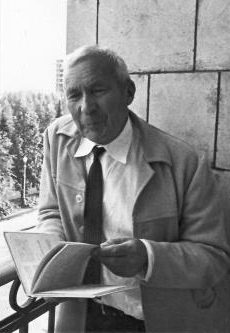
\includegraphics[height=0.36\textheight]{ch0_kolmogorov.jpg}\\[1mm]
\imgcap{Andrei Kolmogorov (1903--1987)}
\imgcredit{https://commons.wikimedia.org/wiki/File:Andrej_Nikolajewitsch_Kolmogorov.jpg}{Foto: Konrad Jacobs; CC BY-SA 2.0 de; Oberwolfach, Wikimedia Commons}\\[1mm]
\raggedright
\begin{itemize}
    \item \textbf{1941}: teoria interpolării și extrapolării șirurilor staționare (\refKolmogorov)
\end{itemize}
\end{column}
\begin{column}{0.48\textwidth}
\centering
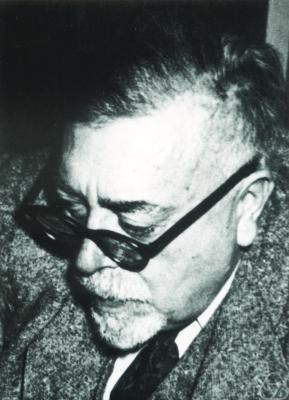
\includegraphics[height=0.36\textheight]{ch0_wiener.jpg}\\[1mm]
\imgcap{Norbert Wiener (1894--1964)}
\imgcredit{https://commons.wikimedia.org/wiki/File:Norbert_wiener.jpg}{Foto: Konrad Jacobs; CC BY-SA 2.0 de; Oberwolfach, Wikimedia Commons}\\[1mm]
\raggedright
\begin{itemize}
    \item \textbf{1942} (raport secret), \textbf{1949}: filtrul Wiener, dezvoltat pentru conducerea tirului antiaerian (\refWiener)
\end{itemize}
\end{column}
\end{columns}
\begin{itemize}
    \item Amîndoi răspund la întrebarea: ce sumă ponderată a valorilor trecute prognozează viitorul cu cea mai mică eroare pătratică medie? Strămoșul filtrului Kalman (\tsachlink{https://danpele.github.io/Time-Series-Analysis/RO/Cursuri/capitol10_spatiul_starilor_kalman_markov_switching.pdf}{Capitolul 10})
\end{itemize}
\end{frame}

\begin{frame}{Box și Jenkins (1970): o metodă pentru practică}
\itemsize{\footnotesize}
\begin{columns}[T]
\begin{column}{0.62\textwidth}
\begin{itemize}
    \item \textbf{1970}: George Box și Gwilym Jenkins publică \emph{Time Series Analysis: Forecasting and Control} (\refBJ)
    \item \textbf{Ciclul Box--Jenkins}
    \begin{itemize}
        \item \textbf{identificare}: alegerea modelului din grafice și din ACF
        \item \textbf{estimare}: estimarea parametrilor
        \item \textbf{verificare}: sînt reziduurile un zgomot imprevizibil?
        \item \textbf{prognoză}: doar după ce verificările au trecut
    \end{itemize}
    \item Modelele ARIMA și versiunea lor sezonieră, SARIMA, provin din această carte (\tsachlink{https://danpele.github.io/Time-Series-Analysis/RO/Cursuri/capitol2_modele_arma.pdf}{Capitolele 2}--\tsachlink{https://danpele.github.io/Time-Series-Analysis/RO/Cursuri/capitol4_sezonalitate_prognoza.pdf}{4})
    \item Box: \emph{toate modelele sînt greșite, dar unele sînt utile}
\end{itemize}
\end{column}
\begin{column}{0.34\textwidth}
\centering
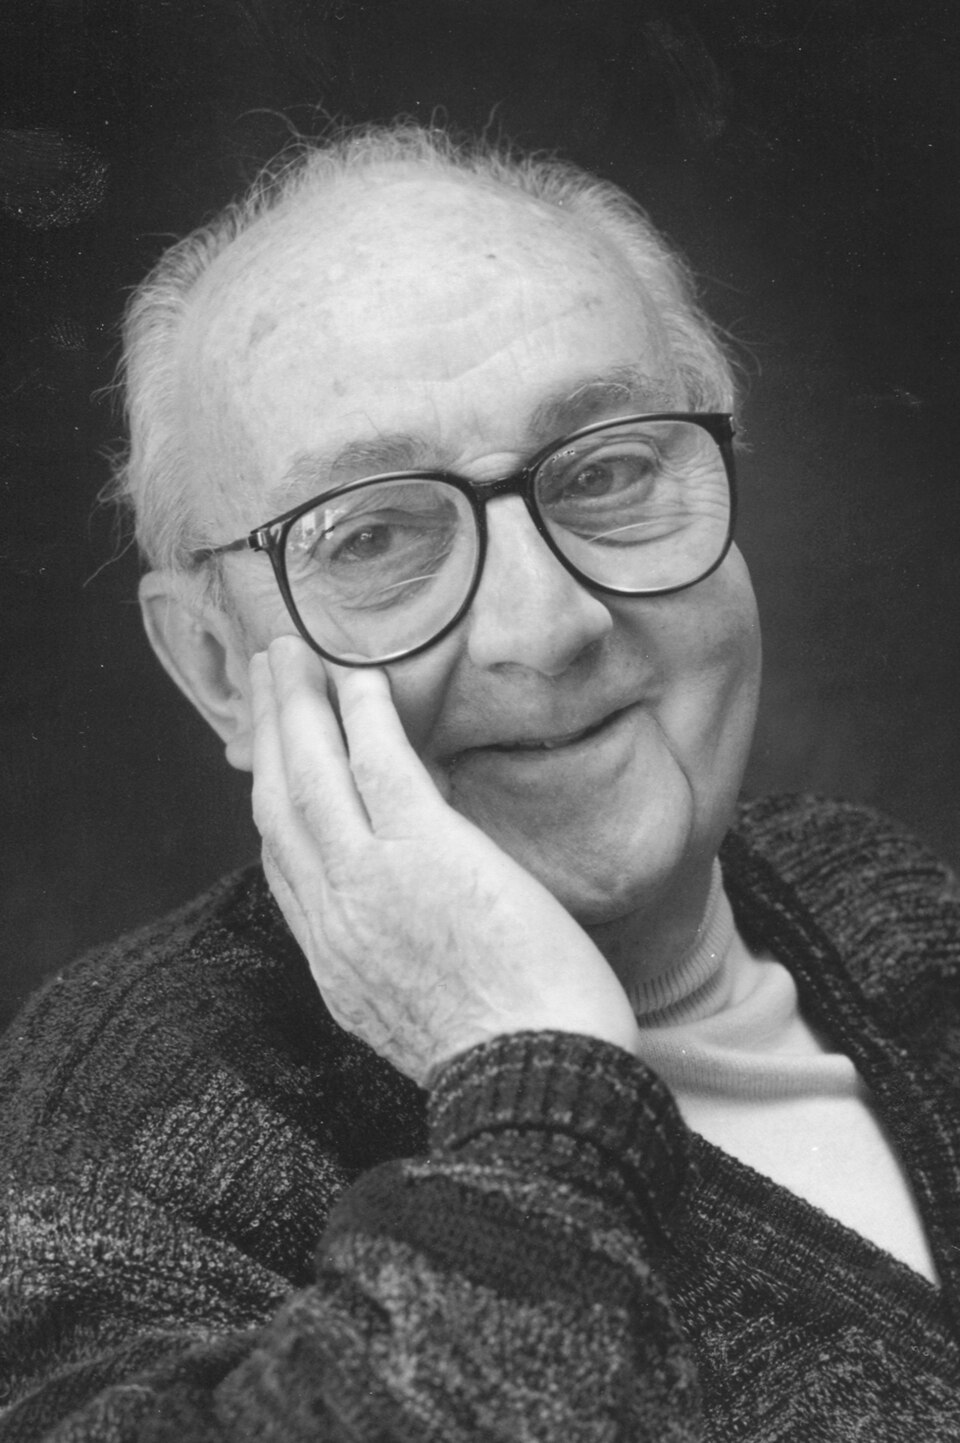
\includegraphics[height=0.52\textheight]{ch0_box.jpg}\\[1mm]
\imgcap{George E.P.\ Box (1919--2013)}
\imgcredit{https://commons.wikimedia.org/wiki/File:GeorgeEPBox_(cropped).jpg}{Foto: DavidMCEddy (2011); CC BY-SA 3.0; Wikimedia Commons}
\end{column}
\end{columns}
\end{frame}

\begin{frame}{Un secol pe o singură axă}
\itemsize{\scriptsize}
\centering
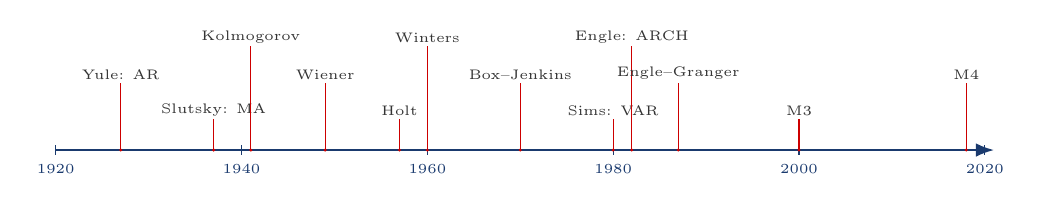
\begin{tikzpicture}[x=0.118cm, y=0.62cm, font=\tiny]
\draw[thick, MainBlue, -{Latex}] (0,0) -- (101,0);
\foreach \x/\y in {0/1920, 20/1940, 40/1960, 60/1980, 80/2000, 100/2020} { \draw[MainBlue] (\x,0.1) -- (\x,-0.1); \node[below, text=MainBlue] at (\x,-0.1) {\y}; }
\foreach \x/\l/\h in {7/{Yule: AR}/1.5, 17/{Slutsky: MA}/0.75, 21/{Kolmogorov}/2.25, 29/{Wiener}/1.5, 37/{Holt}/0.75, 40/{Winters}/2.25, 50/{Box--Jenkins}/1.5, 60/{Sims: VAR}/0.75, 62/{Engle: ARCH}/2.25, 67/{Engle--Granger}/1.5, 80/{M3}/0.75, 98/{M4}/1.5} {
  \draw[IDAred] (\x,0) -- (\x,\h-0.12); \fill[IDAred] (\x,0) circle (0.6pt);
  \node[above, text=DarkGray, inner sep=1pt] at (\x,\h-0.12) {\l};
}
\end{tikzpicture}
\begin{itemize}
    \item 1927 Yule, 1937 Slutsky, 1941 Kolmogorov, 1949 Wiener: fundamentele (\tsachlink{https://danpele.github.io/Time-Series-Analysis/RO/Cursuri/capitol1_procese_stochastice_stationaritate.pdf}{Capitolele 1} și \tsachlink{https://danpele.github.io/Time-Series-Analysis/RO/Cursuri/capitol2_modele_arma.pdf}{2})
    \item 1957 \refHolt, 1960 \refWinters: netezirea exponențială, apărută în industrie, pentru vînzări și stocuri (acest capitol)
    \item 1970 Box--Jenkins (\tsachlink{https://danpele.github.io/Time-Series-Analysis/RO/Cursuri/capitol2_modele_arma.pdf}{Capitolele 2}--\tsachlink{https://danpele.github.io/Time-Series-Analysis/RO/Cursuri/capitol4_sezonalitate_prognoza.pdf}{4}); 1980 \refSims\ (\tsachlink{https://danpele.github.io/Time-Series-Analysis/RO/Cursuri/capitol6_modele_var_cauzalitate_granger.pdf}{Capitolul 6}); 1982 \refEngle\ (\tsachlink{https://danpele.github.io/Time-Series-Analysis/RO/Cursuri/capitol5_volatilitate_conditionata_garch.pdf}{Capitolul 5}); 1987 \refEG\ (\tsachlink{https://danpele.github.io/Time-Series-Analysis/RO/Cursuri/capitol7_cointegrare_vecm.pdf}{Capitolul 7})
    \item 2000 și 2020: competițiile de prognoză M3 și M4 compară metodele pe mii de serii reale (\refMthree; \refMfour)
\end{itemize}
\end{frame}

\begin{frame}{Recapitulare: o scurtă istorie}
\itemsize{\small}
\begin{itemize}
    \item Petele solare (Wolf, 1848) au ridicat prima întrebare: perioade ascunse sau dependență aleatoare?
    \item Yule: o serie explicată prin propriul trecut (AR); Slutsky: sumele de șocuri seamănă cu ciclurile (MA)
    \item Kolmogorov și Wiener: prognoza liniară optimă
    \item Box și Jenkins: identificare, estimare, verificare, prognoză
    \item Competițiile de prognoză: metodele simple sînt greu de depășit
\end{itemize}
\end{frame}


%=============================================================================
\section{Componente și descompunere}
%=============================================================================

\begin{frame}{Patru componente}
\itemsize{\small}
\begin{itemize}
    \item \textbf{Trendul} $T_t$: evoluția pe termen lung a nivelului
    \begin{itemize}
        \item creșterea PIB, creșterea CO2; își poate schimba lent direcția
    \end{itemize}
    \item \textbf{Sezonalitatea} $S_t$: un tipar care se repetă cu o \textbf{perioadă fixă și cunoscută} $m$
    \begin{itemize}
        \item $m = 4$ pentru date trimestriale, $m = 12$ pentru date lunare, $m = 7$ pentru date zilnice cu tipar săptămînal
    \end{itemize}
    \item \textbf{Ciclul} $C_t$: creșteri și scăderi \textbf{fără perioadă fixă}, de obicei mai lungi de un an
    \begin{itemize}
        \item ciclurile economice: expansiuni și recesiuni de 2--10 ani; de obicei sînt unite cu trendul într-o componentă \textbf{trend-ciclu}
    \end{itemize}
    \item \textbf{Componenta neregulată} $R_t$ (reziduală, zgomot): ce rămîne
    \begin{itemize}
        \item ar trebui să pară imprevizibilă; dacă nu, descompunerea a omis ceva
    \end{itemize}
\end{itemize}
\end{frame}

\begin{frame}{Ciclu sau sezonalitate?}
\itemsize{\small}
\begin{itemize}
    \item \textbf{Întrebare pentru sală}: producția de electricitate este mare în fiecare ianuarie
    \begin{itemize}
        \item este un ciclu sau sezonalitate?
    \end{itemize}
    \pause
    \item \textbf{Răspuns}: sezonalitate: perioada este fixă (12 luni) și cunoscută dinainte
    \begin{itemize}
        \item o recesiune apare într-un moment necunoscut și durează un timp necunoscut: acesta este un ciclu
    \end{itemize}
    \item \textbf{Importanța diferenței}
    \begin{itemize}
        \item sezonalitatea poate fi prognozată cu ani înainte: și luna ianuarie viitoare va avea valori mari
        \item ciclurile se prognozează greu: momentul lor se schimbă (Slutsky)
        \item petele solare: un \emph{ciclu} de 11 ani, nu o sezonalitate, pentru că durata lui variază
    \end{itemize}
\end{itemize}
\end{frame}

\begin{frame}{Modelul aditiv și modelul multiplicativ}
\itemsize{\small}
\begin{itemize}
    \item \textbf{Aditiv}: $y_t = T_t + S_t + R_t$
    \begin{itemize}
        \item oscilația sezonieră are o mărime constantă, în unitățile lui $y$ (CO2: cîțiva ppm în fiecare an)
    \end{itemize}
    \item \textbf{Multiplicativ}: $y_t = T_t \times S_t \times R_t$
    \begin{itemize}
        \item oscilația sezonieră este un \textbf{procent} constant din nivel (PIB: trimestrul I cu aproximativ un sfert sub trend)
        \item $S_t$ și $R_t$ sînt factori în jurul lui 1: $S_t = 0{,}8$ înseamnă 20\% sub trend
    \end{itemize}
    \item \textbf{Logaritmul le leagă}: $\ln y_t = \ln T_t + \ln S_t + \ln R_t$
    \begin{itemize}
        \item o serie multiplicativă devine aditivă după logaritmare
    \end{itemize}
    \item \textbf{Alegerea}: priviți graficul
    \begin{itemize}
        \item oscilația sezonieră crește odată cu nivelul? Multiplicativ (sau logaritmi); altfel, aditiv
    \end{itemize}
\end{itemize}
\end{frame}

\begin{frame}{Medii mobile centrate}
\itemsize{\small}
\begin{itemize}
    \item \textbf{Media mobilă de ordin} $k$ (impar): media a $k$ valori vecine
    \begin{itemize}
        \item $\hat T_t = \frac{1}{k} \sum_{j=-q}^{q} y_{t+j}$, cu $k = 2q + 1$; netezește zgomotul
        \item $q$: numărul de valori de fiecare parte a lui $t$; $j$: poziția față de $t$; căciula marchează o estimare
    \end{itemize}
    \item \textbf{Proprietatea esențială}: o medie mobilă pe un sezon complet elimină tiparul sezonier
    \begin{itemize}
        \item fiecare trimestru intră o singură dată, deci efectele sezoniere se compensează
    \end{itemize}
    \item \textbf{Perioadă pară} $m = 4$: o medie mobilă $2 \times 4$, pentru a rămîne centrată pe un trimestru
    \begin{itemize}
        \item $\hat T_t = \frac{1}{8} y_{t-2} + \frac{1}{4} y_{t-1} + \frac{1}{4} y_t + \frac{1}{4} y_{t+1} + \frac{1}{8} y_{t+2}$
        \item cinci trimestre, cele două capete cu pondere înjumătățită; pentru date lunare, $2 \times 12$
    \end{itemize}
    \item Primele și ultimele $m/2$ valori nu au medie centrată: estimarea trendului lipsește la ambele capete
\end{itemize}
\end{frame}

\begin{frame}{Exemplu rezolvat: o medie mobilă $2 \times 4$}
\itemsize{\footnotesize}
\begin{columns}[T]
\begin{column}{0.32\textwidth}
\begin{center}
\footnotesize
\begin{tabular}{lr}
\toprule
\textbf{Trimestru} & \textbf{$y_t$} \\
\midrule
T1 2024 & 38{,}7 \\
T2 2024 & 45{,}6 \\
T3 2024 & 52{,}8 \\
T4 2024 & 59{,}2 \\
T1 2025 & 38{,}9 \\
\bottomrule
\end{tabular}
\end{center}

\end{column}
\begin{column}{0.64\textwidth}
\begin{itemize}
    \item PIB-ul real al României, miliarde EUR (Eurostat, neajustat)
    \item \textbf{Trendul în T3 2024}
    \begin{itemize}
        \item $\hat T_t = \frac{1}{4}\left(\frac{38{,}7}{2} + 45{,}6 + 52{,}8 + 59{,}2 + \frac{38{,}9}{2}\right) = 49{,}10$
    \end{itemize}
    \item \textbf{Raportul sezonier}
    \begin{itemize}
        \item $y_t / \hat T_t = 52{,}8 / 49{,}10$: trimestrul III este peste trend
    \end{itemize}
    \item Media acestor rapoarte pe toți anii oferă factorul sezonier al fiecărui trimestru
\end{itemize}
\end{column}
\end{columns}
\end{frame}

\begin{frame}{Descompunerea clasică, pas cu pas}
\itemsize{\small}
\begin{itemize}
    \item \textbf{Pasul 1}: trend-ciclul $\hat T_t$, printr-o medie mobilă centrată $2 \times m$
    \item \textbf{Pasul 2}: eliminarea trendului
    \begin{itemize}
        \item multiplicativ: $y_t / \hat T_t$; aditiv: $y_t - \hat T_t$
    \end{itemize}
    \item \textbf{Pasul 3}: factorii sezonieri $\hat S_1, \ldots, \hat S_m$
    \begin{itemize}
        \item media valorilor fără trend din fiecare sezon, pe toți anii
        \item normalizare: media lor este 1 (multiplicativ) sau 0 (aditiv)
    \end{itemize}
    \item \textbf{Pasul 4}: componenta neregulată $\hat R_t = y_t / (\hat T_t \hat S_t)$ sau $y_t - \hat T_t - \hat S_t$
    \item \textbf{Seria ajustată sezonier}: $y_t / \hat S_t$ sau $y_t - \hat S_t$
    \begin{itemize}
        \item limite: același tipar sezonier în fiecare an, fără trend la capete, sensibilitate la valori extreme
    \end{itemize}
\end{itemize}
\end{frame}

\begin{frame}{Descompunerea PIB-ului României}
\itemsize{\footnotesize}
\begin{center}
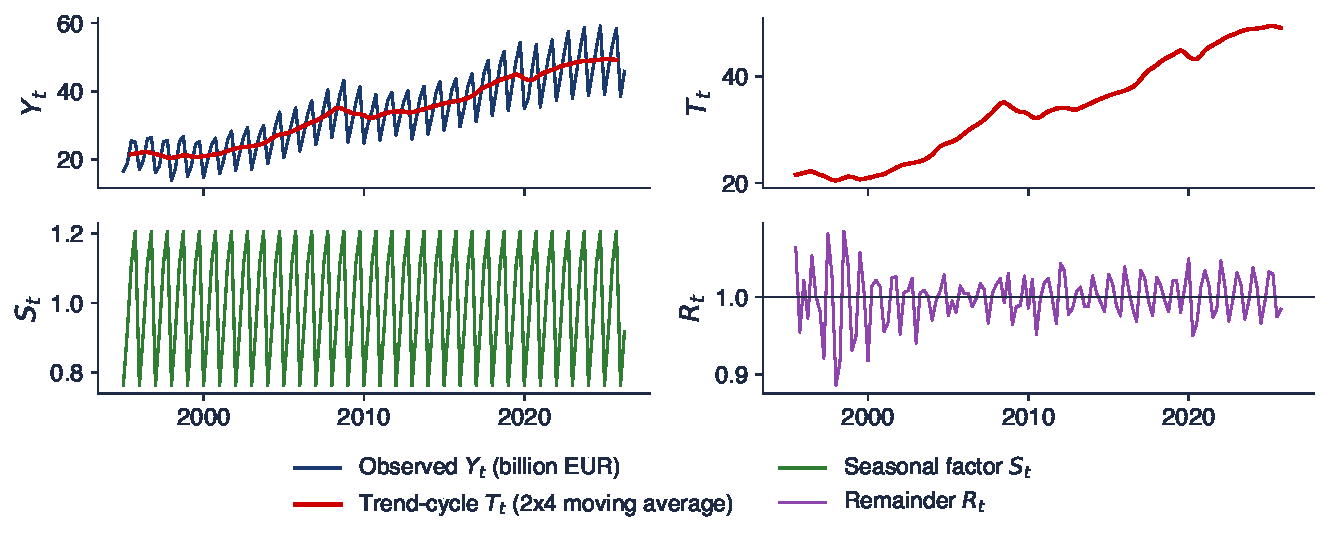
\includegraphics[width=0.94\textwidth,height=0.66\textheight,keepaspectratio]{tsa_ch0_components.pdf}
\end{center}
\vspace{-2mm}
\begin{itemize}
    \item Descompunere clasică multiplicativă, $m = 4$: seria observată și trend-ciclul, trend-ciclul, factorii sezonieri, componenta neregulată
\end{itemize}
\quantlet{TSA\_ch0\_decomposition}{\qlurl{TSA_ch0_decomposition}}
\end{frame}

\begin{frame}{Interpretarea: factorii sezonieri ai PIB}
\itemsize{\footnotesize}
\begin{columns}[T]
\begin{column}{0.36\textwidth}
\begin{center}
\footnotesize
\begin{tabular}{lrr}
\toprule
\textbf{Trimestru} & $\hat S_q$ & față de trend \\
\midrule
T1 & 0{,}762 & $\ensuremath{-}23{,}8$\% \\
T2 & 0{,}918 & $\ensuremath{-}8{,}2$\% \\
T3 & 1{,}113 & $+$11{,}3\% \\
T4 & 1{,}207 & $+$20{,}7\% \\
\bottomrule
\end{tabular}
\end{center}

\end{column}
\begin{column}{0.60\textwidth}
\begin{itemize}
    \item \textbf{Citirea factorilor}
    \begin{itemize}
        \item $\hat S_q$: factorul sezonier estimat al trimestrului $q$
        \item un trimestru I tipic se află cu 23{,}8\% sub trend, un trimestru IV tipic cu 20{,}7\% peste trend
        \item trimestrul IV este cu aproximativ 58\% mai mare decît trimestrul I, din motive pur sezoniere
    \end{itemize}
    \item \textbf{Componenta neregulată}
    \begin{itemize}
        \item abaterea standard este de aproximativ 3{,}3\%; mai mare în anii 1990 și în 2020
    \end{itemize}
    \item Consecință: comparați un trimestru cu același trimestru din anul anterior, niciodată cu trimestrul precedent al seriei neajustate
\end{itemize}
\end{column}
\end{columns}
\end{frame}

\begin{frame}{STL: o descompunere flexibilă}
\itemsize{\small}
\begin{itemize}
    \item \textbf{STL}: Seasonal and Trend decomposition using LOESS, descompunere în sezonalitate și trend cu LOESS (\refSTL)
    \begin{itemize}
        \item LOESS (locally estimated scatterplot smoothing): o regresie ponderată, estimată în jurul fiecărui punct
    \end{itemize}
    \item \textbf{Avantaje față de metoda clasică}
    \begin{itemize}
        \item tiparul sezonier se poate schimba lent de la un an la altul
        \item o estimare a trendului pînă la ultima observație
        \item o variantă robustă: valorile extreme ajung în componenta neregulată și nu deformează sezonalitatea
    \end{itemize}
    \item \textbf{Limite}
    \begin{itemize}
        \item doar aditivă: pentru serii multiplicative se aplică lui $\ln y_t$
        \item nu tratează efectele de calendar (zile lucrătoare, Paște)
    \end{itemize}
    \item Institutele de statistică folosesc X-13ARIMA-SEATS sau TRAMO-SEATS, metode construite pe modele ARIMA (\tsachlink{https://danpele.github.io/Time-Series-Analysis/RO/Cursuri/capitol4_sezonalitate_prognoza.pdf}{Capitolul 4})
\end{itemize}
\end{frame}

\begin{frame}{Descompunerea STL a seriei CO2}
\itemsize{\footnotesize}
\begin{center}
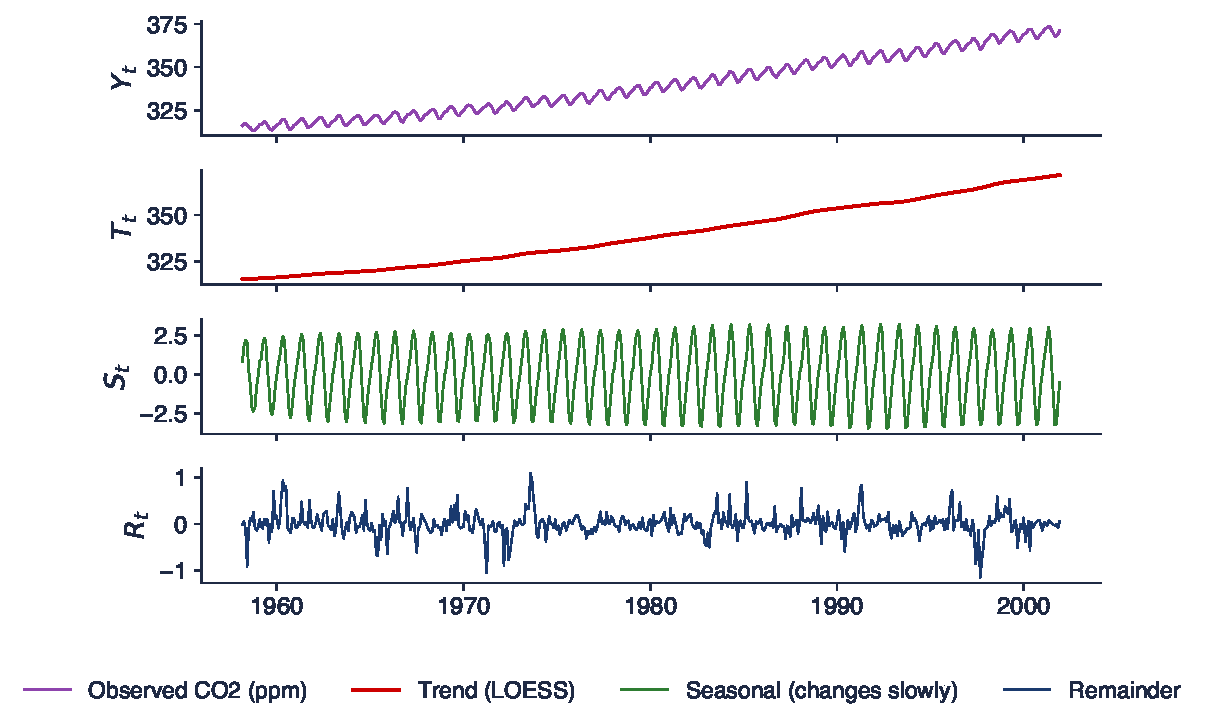
\includegraphics[width=0.94\textwidth,height=0.66\textheight,keepaspectratio]{tsa_ch0_stl.pdf}
\end{center}
\vspace{-2mm}
\begin{itemize}
    \item STL robustă cu perioada 12, pe seria lunară CO2: seria observată, trendul, sezonalitatea, componenta neregulată (ppm)
\end{itemize}
\quantlet{TSA\_ch0\_decomposition}{\qlurl{TSA_ch0_decomposition}}
\end{frame}

\begin{frame}{Interpretarea: STL pentru CO2}
\itemsize{\small}
\begin{itemize}
    \item \textbf{Trendul}: neted, ușor convex: creșterea se accelerează
    \item \textbf{Sezonalitatea}: maximul în mai, minimul în octombrie
    \begin{itemize}
        \item iarna și primăvara: descompunerea frunzelor căzute eliberează CO2; vara: fotosinteza îl absoarbe
        \item amplitudinea anuală crește de la 4{,}9 ppm (1959) la 6{,}3 ppm (2001): STL permite modificarea sezonalității
    \end{itemize}
    \item \textbf{Componenta neregulată}: abaterea standard 0{,}25 ppm
    \begin{itemize}
        \item mică în raport cu sezonalitatea: trendul și sezonalitatea explică aproape totul
        \item verificați vîrfurile mai mari în istoricul stației înainte de a le considera zgomot
    \end{itemize}
\end{itemize}
\end{frame}

\begin{frame}{Recapitulare: componente și descompunere}
\itemsize{\small}
\begin{itemize}
    \item Trend, sezonalitate (perioadă fixă), ciclu (fără perioadă fixă), componenta neregulată
    \item Aditiv dacă oscilația sezonieră este constantă, multiplicativ dacă ea crește odată cu nivelul; logaritmul transformă un model în celălalt
    \item O medie mobilă centrată $2 \times m$ elimină sezonalitatea și estimează trend-ciclul
    \item PIB-ul României: trimestrul I cu aproximativ 23{,}8\% sub trend, trimestrul IV cu aproximativ 20{,}7\% peste trend
    \item STL permite modificarea tiparului sezonier și este robustă la valori extreme
\end{itemize}
\end{frame}


%=============================================================================
\section{Notație, transformări și ACF}
%=============================================================================

\begin{frame}{Notația folosită în curs}
\itemsize{\footnotesize}
\begin{center}
\footnotesize
\begin{tabular}{>{\raggedright\arraybackslash}p{3.2cm}>{\raggedright\arraybackslash}p{8.8cm}}
\toprule
\textbf{Simbol} & \textbf{Semnificație} \\
\midrule
$y_t$, $t = 1, \ldots, T$ & observația din momentul $t$; $T$ observații în eșantion \\
$\bar y = \frac1T \sum_t y_t$ & media de selecție \\
$L y_t = y_{t-1}$ & \textbf{operatorul lag}: deplasează seria cu o perioadă înapoi; $L^k y_t = y_{t-k}$ \\
$\Delta y_t = y_t - y_{t-1}$ & \textbf{diferența de ordinul întîi}, $\Delta = 1 - L$ \\
$\Delta_m y_t = y_t - y_{t-m}$ & \textbf{diferența sezonieră}, $\Delta_m = 1 - L^m$ \\
$\hat y_{T+h|T}$ & prognoza lui $y_{T+h}$ făcută cu datele pînă la $T$; $h$ este \textbf{orizontul} \\
$e_t = y_t - \hat y_t$ & eroarea de prognoză \\
\bottomrule
\end{tabular}
\end{center}
\begin{itemize}
    \item Căciula ($\hat{\ }$) marchează estimările și prognozele; literele grecești ($\phi, \theta, \alpha$) marchează parametrii
\end{itemize}
\end{frame}

\begin{frame}{Transformări: logaritmi, diferențe, rate de creștere}
\itemsize{\footnotesize}
\begin{itemize}
    \item \textbf{Logaritmul} $\ln y_t$: stabilizează o varianță care crește odată cu nivelul
    \item \textbf{Rata de creștere pe o perioadă}: $g_t = 100\,(y_t / y_{t-1} - 1)$
    \begin{itemize}
        \item aproximarea logaritmică: $100\,\Delta \ln y_t \approx g_t$ pentru variații mici
    \end{itemize}
    \item \textbf{Rata anuală de creștere} a unei serii trimestriale: $100\,(y_t / y_{t-4} - 1)$
    \begin{itemize}
        \item compară aceleași trimestre, deci sezonalitatea se anulează
    \end{itemize}
    \item \textbf{Exemplu rezolvat}: PIB-ul României, T1 2024 = 38{,}7, T4 2024 = 59{,}2, T1 2025 = 38{,}9
    \begin{itemize}
        \item pe un trimestru: $100\,(38{,}9 / 59{,}2 - 1) \approx -34\%$: nu o prăbușire, ci doar iarna
        \item pe un an: $100\,(38{,}9 / 38{,}7 - 1) \approx +0{,}5\%$: economia aproape nu a crescut
    \end{itemize}
    \item \textbf{Randamentul logaritmic} al unui preț: $r_t = 100\,(\ln P_t - \ln P_{t-1})$, în \%; $P_t$: prețul din ziua $t$
\end{itemize}
\end{frame}

\begin{frame}{De la prețuri la randamente: BET}
\itemsize{\footnotesize}
\begin{center}
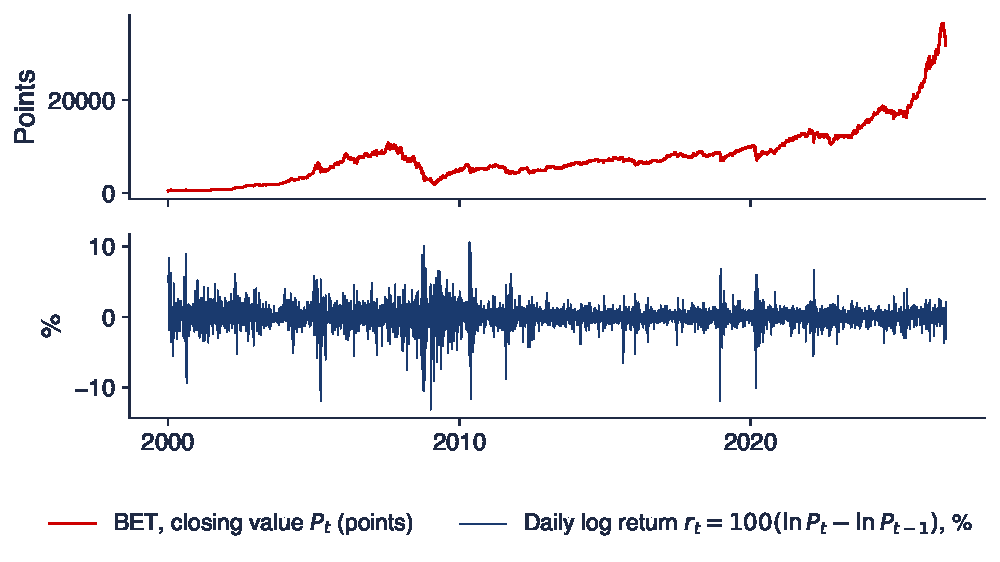
\includegraphics[width=0.94\textwidth,height=0.6\textheight,keepaspectratio]{tsa_ch0_returns.pdf}
\end{center}
\vspace{-2mm}
\begin{itemize}
    \item Sus: valoarea de închidere a indicelui BET din 2000; jos: randamentele logaritmice zilnice, în \% (6\,670 de zile de tranzacționare)
\end{itemize}
\quantlet{TSA\_ch0\_acf}{\qlurl{TSA_ch0_acf}}
\end{frame}

\begin{frame}{Interpretarea: prețuri și randamente}
\itemsize{\small}
\begin{itemize}
    \item \textbf{Prețul are trend; randamentele nu au}
    \begin{itemize}
        \item randamentele fluctuează în jurul unei medii de 0{,}064\% pe zi, cu abaterea standard de 1{,}40\% (aproximativ 22\% pe an)
    \end{itemize}
    \item \textbf{Zile extreme}
    \begin{itemize}
        \item cea mai slabă: \ensuremath{-}13{,}1\% pe 7 ianuarie 2009; cea mai bună: +10{,}6\% pe 10 mai 2010
    \end{itemize}
    \item \textbf{Perioadele calme alternează cu cele agitate}
    \begin{itemize}
        \item variațiile mari apar grupat în 2008--2010 și în martie 2020: \emph{volatility clustering} (\tsachlink{https://danpele.github.io/Time-Series-Analysis/RO/Cursuri/capitol5_volatilitate_conditionata_garch.pdf}{Capitolul 5})
    \end{itemize}
    \item Diferențierea logaritmului prețului elimină trendul: majoritatea modelelor din curs se aplică unor astfel de serii transformate
\end{itemize}
\end{frame}

\begin{frame}{Funcția de autocorelație de selecție}
\itemsize{\small}
\begin{itemize}
    \item \textbf{Întrebarea}: cît de puternic este legat $y_t$ de propria valoare de acum $k$ perioade?
    \item \textbf{Autocovarianța de selecție} la lagul $k$
    \begin{itemize}
        \item $c_k = \frac{1}{T} \sum_{t=k+1}^{T} (y_t - \bar y)(y_{t-k} - \bar y)$
        \item $k$: lagul, în perioade; $\bar y$: media de selecție; produsul este pozitiv cînd $y_t$ și $y_{t-k}$ se află de aceeași parte a mediei
    \end{itemize}
    \item \textbf{Autocorelația de selecție}: $r_k = c_k / c_0$, între $-1$ și $1$
    \begin{itemize}
        \item $c_0$: varianța de selecție (autocovarianța la lagul 0)
        \item \textbf{ACF} (autocorrelation function, funcția de autocorelație) este șirul $r_1, r_2, \ldots$ reprezentat în funcție de $k$ (\textbf{corelograma})
    \end{itemize}
    \item \textbf{Banda de referință} $\pm 1{,}96 / \sqrt{T}$
    \begin{itemize}
        \item dacă seria ar fi un zgomot independent, aproximativ 95\% dintre valorile $r_k$ ar cădea în interiorul ei; 1,96: cuantila de 97,5\% a distribuției Normale standard
        \item teoria (staționaritate, zgomot alb, testul Ljung--Box) urmează în \tsachlink{https://danpele.github.io/Time-Series-Analysis/RO/Cursuri/capitol1_procese_stochastice_stationaritate.pdf}{Capitolul 1}
    \end{itemize}
\end{itemize}
\end{frame}

\begin{frame}{Exemplu rezolvat: $r_1$ calculat de mînă}
\itemsize{\footnotesize}
\begin{columns}[T]
\begin{column}{0.48\textwidth}
\begin{center}
\footnotesize
\begin{tabular}{rrrr}
\toprule
$t$ & $y_t$ & $y_t - \bar y$ & $(y_t - \bar y)(y_{t-1} - \bar y)$ \\
\midrule
1 & 2 & $-2$ & -- \\
2 & 4 & $0$ & $0$ \\
3 & 3 & $-1$ & $0$ \\
4 & 5 & $1$ & $-1$ \\
5 & 4 & $0$ & $0$ \\
6 & 6 & $2$ & $0$ \\
\midrule sumă & 24 & 0 & $-1$ \\
\bottomrule
\end{tabular}
\end{center}

\end{column}
\begin{column}{0.48\textwidth}
\begin{itemize}
    \item $T = 6$, $\bar y = 24 / 6 = 4$
    \item suma pătratelor abaterilor: $4 + 0 + 1 + 1 + 0 + 4 = 10$
    \item $r_1 = \dfrac{-1/6}{10/6} = -0{,}1$
    \item la lagul 2: produsele $(-1)(-2) + (1)(0) + (0)(-1) + (2)(1) = 4$, deci $r_2 = 0{,}4$
    \item \textbf{Interpretare}
    \begin{itemize}
        \item banda $\pm 1{,}96/\sqrt 6 = \pm 0{,}80$: cu 6 observații, nicio valoare nu se deosebește de 0
    \end{itemize}
\end{itemize}
\end{column}
\end{columns}
\end{frame}

\begin{frame}{Trei corelograme}
\itemsize{\footnotesize}
\begin{center}
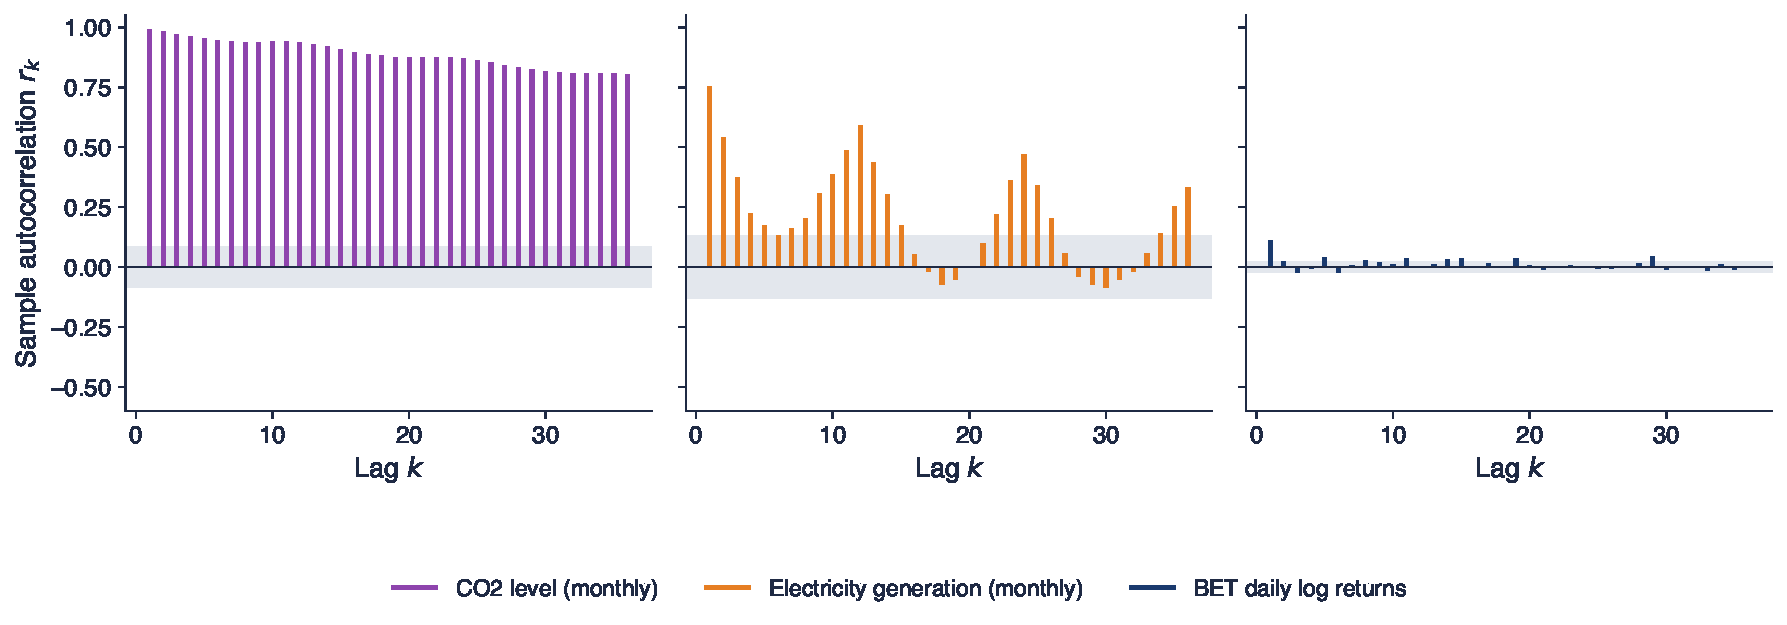
\includegraphics[width=0.94\textwidth,height=0.5\textheight,keepaspectratio]{tsa_ch0_acf.pdf}
\end{center}
\vspace{-2mm}
\begin{itemize}
    \item ACF de selecție pentru lagurile 1--36; zona colorată: banda $\pm 1{,}96/\sqrt{T}$. Stînga: nivelul CO2; centru: producția lunară de electricitate; dreapta: randamentele logaritmice zilnice ale BET
\end{itemize}
\quantlet{TSA\_ch0\_acf}{\qlurl{TSA_ch0_acf}}
\end{frame}

\begin{frame}{Interpretarea: trei corelograme}
\itemsize{\small}
\begin{itemize}
    \item \textbf{Trend}: CO2, $r_1 = $ 0{,}993, încă 0{,}80 la lagul 36
    \begin{itemize}
        \item o descreștere lentă, aproape liniară, este semnătura unui trend: nivelul rămîne corelat cu valorile de acum cîțiva ani
    \end{itemize}
    \item \textbf{Sezonalitate}: electricitatea, $r_6 = $ 0{,}13, $r_{12} = $ 0{,}59
    \begin{itemize}
        \item vîrfuri la 12, 24 și 36 de luni: luna ianuarie de anul acesta seamănă cu ianuarie de anul trecut
    \end{itemize}
    \item \textbf{Aproape fără memorie}: randamentele BET, $r_1 = $ 0{,}109, $r_2 = $ 0{,}022, banda $\pm$0{,}024
    \begin{itemize}
        \item autocorelații mici, dar semnificative: greu de exploatat după costurile de tranzacționare
        \item randamentele în valoare \emph{absolută} au $r_1 = $ 0{,}40: mărimea variațiilor este previzibilă, semnul lor mult mai puțin (\tsachlink{https://danpele.github.io/Time-Series-Analysis/RO/Cursuri/capitol5_volatilitate_conditionata_garch.pdf}{Capitolul 5})
    \end{itemize}
    \item ACF a unei serii cu trend este puțin informativă: întîi transformați seria, apoi examinați ACF
\end{itemize}
\end{frame}

\begin{frame}{Recapitulare: notație, transformări și ACF}
\itemsize{\small}
\begin{itemize}
    \item $L y_t = y_{t-1}$, $\Delta = 1 - L$, $\Delta_m = 1 - L^m$; $\hat y_{T+h|T}$ este prognoza pentru orizontul $h$
    \item Logaritmii stabilizează varianța; diferențele elimină trendul; ratele anuale elimină sezonalitatea
    \item $r_k = c_k / c_0$, comparat cu banda $\pm 1{,}96/\sqrt T$
    \item Descreștere lentă: trend; vîrfuri la $m, 2m, \ldots$: sezonalitate; toate aproape de 0: memorie liniară redusă
\end{itemize}
\end{frame}


%=============================================================================
\section{Netezirea exponențială}
%=============================================================================

\begin{frame}{Netezirea exponențială simplă (SES)}
\itemsize{\small}
\begin{itemize}
    \item \textbf{Ideea}: prognoza este o medie ponderată a trecutului, în care valorile recente au ponderi mai mari
    \item \textbf{Ecuația nivelului}: $\ell_t = \alpha y_t + (1 - \alpha)\, \ell_{t-1}$, cu $0 < \alpha \le 1$
    \begin{itemize}
        \item $\ell_t$: nivelul netezit în momentul $t$; $\alpha$: constanta de netezire; $\ell_t$ se deplasează de la $\ell_{t-1}$ spre $y_t$ cu fracțiunea $\alpha$
        \item prognoza pentru orice orizont: $\hat y_{T+h|T} = \ell_T$, o dreaptă orizontală
    \end{itemize}
    \item \textbf{Originea denumirii „exponențială”}: substituiri repetate
    \begin{itemize}
        \item $\ell_T = \alpha y_T + \alpha(1-\alpha) y_{T-1} + \alpha(1-\alpha)^2 y_{T-2} + \cdots$
        \item ponderile scad geometric; cu $\alpha = 0{,}5$: 0,5; 0,25; 0,125; \ldots
    \end{itemize}
    \item \textbf{Constanta de netezire} $\alpha$
    \begin{itemize}
        \item $\alpha$ mic: memorie lungă, prognoze netede, reacție lentă; $\alpha = 1$: prognoza naivă $\hat y_{T+1} = y_T$
        \item se estimează prin minimizarea sumei pătratelor erorilor de prognoză cu un pas înainte
    \end{itemize}
\end{itemize}
\end{frame}

\begin{frame}{Exemplu rezolvat: SES cu $\alpha = 0{,}5$}
\itemsize{\footnotesize}
\begin{columns}[T]
\begin{column}{0.52\textwidth}
\begin{center}
\footnotesize
\begin{tabular}{rrrr}
\toprule
$t$ & $y_t$ & $\hat y_{t|t-1} = \ell_{t-1}$ & $\ell_t = 0{,}5\,y_t + 0{,}5\,\ell_{t-1}$ \\
\midrule
0 & -- & -- & $\ell_0 = 10$ \\
1 & 10 & 10 & 10 \\
2 & 12 & 10 & 11 \\
3 & 11 & 11 & 11 \\
4 & 13 & 11 & 12 \\
5 & ? & \textbf{12} & -- \\
\bottomrule
\end{tabular}
\end{center}

\end{column}
\begin{column}{0.44\textwidth}
\begin{itemize}
    \item nivelul inițial $\ell_0 = 10$ (prima observație)
    \item $t = 2$: $0{,}5 \times 12 + 0{,}5 \times 10 = 11$
    \item $t = 4$: $0{,}5 \times 13 + 0{,}5 \times 11 = 12$
    \item \textbf{Interpretare}
    \begin{itemize}
        \item prognoza pentru $t = 5$ și pentru toate perioadele următoare este 12: SES nu extrapolează trendul
        \item erorile cu un pas: 0, 2, 0, 2: prognozele rămîn în urma datelor crescătoare
    \end{itemize}
\end{itemize}
\end{column}
\end{columns}
\end{frame}

\begin{frame}{SES pe cursul EUR/RON lunar}
\itemsize{\footnotesize}
\begin{center}
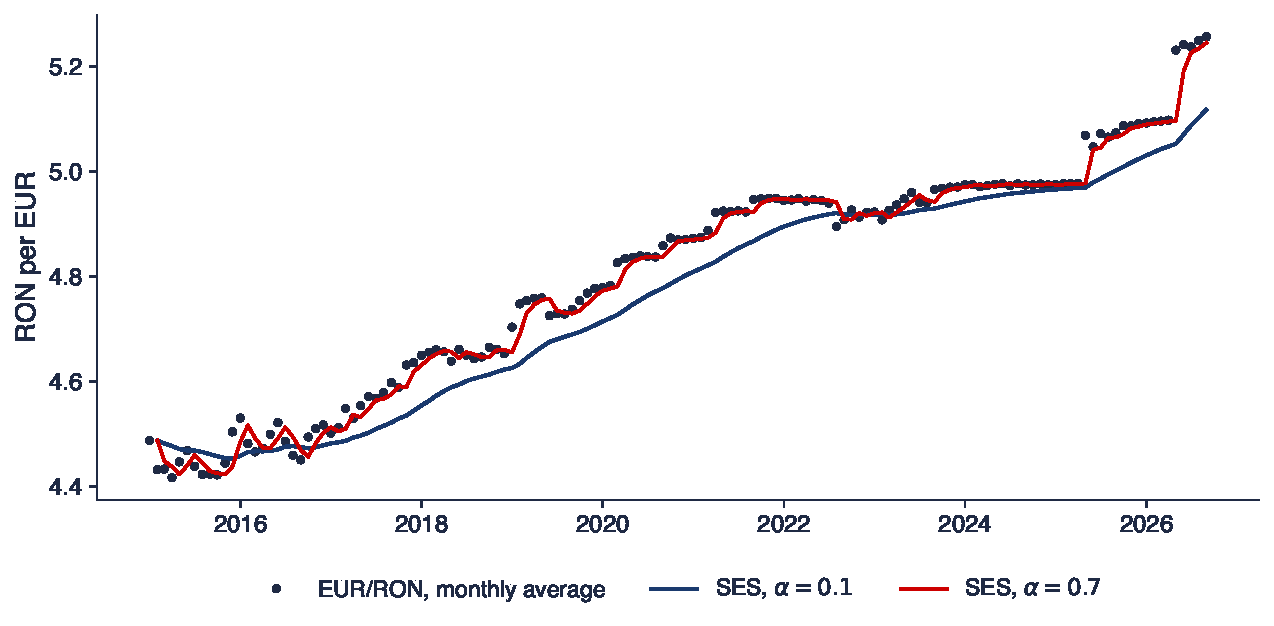
\includegraphics[width=0.94\textwidth,height=0.58\textheight,keepaspectratio]{tsa_ch0_ses.pdf}
\end{center}
\vspace{-2mm}
\begin{itemize}
    \item Puncte: mediile lunare ale cursului de referință BNR, ianuarie 2015 -- septembrie 2026; linii: prognozele SES cu un pas, $\hat y_{t|t-1}$, cu $\alpha = 0{,}1$ și $\alpha = 0{,}7$
\end{itemize}
\quantlet{TSA\_ch0\_smoothing}{\qlurl{TSA_ch0_smoothing}}
\end{frame}

\begin{frame}{Interpretarea: alegerea lui $\alpha$}
\itemsize{\small}
\begin{itemize}
    \item \textbf{$\alpha = 0{,}1$}: netedă, dar mereu sub cursul crescător
    \begin{itemize}
        \item ponderează observații din mai mulți ani: după saltul din 2025 are nevoie de multe luni pentru a ajunge la noul nivel
    \end{itemize}
    \item \textbf{$\alpha = 0{,}7$}: urmărește îndeaproape datele, cu o lună întîrziere
    \item \textbf{Valoarea estimată} $\hat\alpha = $ 1{,}00
    \begin{itemize}
        \item cea mai bună prognoză SES pentru luna viitoare este media lunii curente: SES se reduce la prognoza naivă
        \item tipic pentru cursurile de schimb și prețuri: ultima valoare conține aproape toată informația (un mers aleator, \tsachlink{https://danpele.github.io/Time-Series-Analysis/RO/Cursuri/capitol1_procese_stochastice_stationaritate.pdf}{Capitolul 1})
    \end{itemize}
    \item O valoare estimată a lui $\alpha$ apropiată de 1 este o informație despre serie, nu un eșec al metodei
\end{itemize}
\end{frame}

\begin{frame}{Metodele Holt și Holt--Winters (1/2)}
\itemsize{\footnotesize}
\begin{itemize}
    \item \textbf{Holt (1957)}: nivel și \textbf{trend} $b_t$ (\refHolt)
    \begin{itemize}
        \item $\ell_t = \alpha y_t + (1-\alpha)(\ell_{t-1} + b_{t-1})$, \ $b_t = \beta (\ell_t - \ell_{t-1}) + (1-\beta) b_{t-1}$
        \item nivelul se actualizează spre $y_t$, pornind de la nivelul anterior plus panta anterioară
        \item $b_t$: panta estimată, adică variația nivelului pe perioadă; se actualizează spre ultima variație $\ell_t - \ell_{t-1}$
        \item $\beta \in (0, 1]$: constanta de netezire a pantei; un $\beta$ mic dă o pantă care se schimbă lent
    \end{itemize}
    \item \textbf{Prognoza}: $\hat y_{T+h|T} = \ell_T + h\, b_T$, o dreaptă
    \begin{itemize}
        \item ultimul nivel plus de $h$ ori ultima pantă
        \item un trend \textbf{amortizat} înmulțește panta cu $\phi^j$, $0 < \phi < 1$, la pasul $j$: dreapta se aplatizează pentru orizonturi lungi
    \end{itemize}
\end{itemize}
\end{frame}

\begin{frame}{Metodele Holt și Holt--Winters (2/2)}
\itemsize{\footnotesize}
\begin{itemize}
    \item \textbf{Holt--Winters (1960)}: adaugă factori sezonieri $s_t$ cu perioada $m$ (\refWinters)
    \begin{itemize}
        \item forma multiplicativă: $\hat y_{T+h|T} = (\ell_T + h\, b_T)\, s_{T+h-m}$
        \item $s_{T+h-m}$: ultimul factor sezonier al aceluiași sezon (pentru $h \le m$); $s = 1{,}1$ înseamnă 10\% peste linia trendului
        \item fiecare componentă are propria constantă de netezire: $\alpha$ (nivel), $\beta$ (pantă), $\gamma$ (sezonalitate)
    \end{itemize}
    \item \textbf{ETS}: Error, Trend, Seasonal, adică eroare, trend, sezonalitate (\refHKSG)
    \begin{itemize}
        \item fiecare metodă este un model statistic: N (none, absent), A (aditiv), M (multiplicativ), A$_d$ (amortizat)
        \item de exemplu, ETS(M,A$_d$,M): erori multiplicative, trend amortizat, sezonalitate multiplicativă; oferă intervale de prognoză și un criteriu informațional (\tsachlink{https://danpele.github.io/Time-Series-Analysis/RO/Cursuri/capitol2_modele_arma.pdf}{Capitolul 2})
    \end{itemize}
    \item O sinteză a 25 de ani de netezire exponențială: \refGardner
\end{itemize}
\end{frame}

\begin{frame}{Recapitulare: netezirea exponențială}
\itemsize{\small}
\begin{itemize}
    \item SES: $\ell_t = \alpha y_t + (1-\alpha)\ell_{t-1}$; ponderile scad geometric; prognoze orizontale
    \item $\alpha$ mic: netezire puternică și reacție lentă; $\alpha = 1$: prognoza naivă
    \item EUR/RON: $\hat\alpha = $ 1{,}00, ultima valoare este cea mai bună prognoză SES
    \item Holt adaugă un trend, Holt--Winters o sezonalitate; ETS le transformă în modele statistice
\end{itemize}
\end{frame}


%=============================================================================
\section{Prognoza și evaluarea ei}
%=============================================================================

\begin{frame}{Prognoza: cadrul general}
\itemsize{\small}
\begin{itemize}
    \item \textbf{Prognoza} $\hat y_{T+h|T}$: o afirmație despre $y_{T+h}$, făcută în momentul $T$
    \begin{itemize}
        \item poate folosi doar informația disponibilă în momentul $T$: \textbf{mulțimea de informație}
        \item $h = 1, 2, \ldots$: \textbf{orizontul}; incertitudinea crește odată cu $h$
    \end{itemize}
    \item \textbf{Prognoze punctuale și prognoze pe interval}
    \begin{itemize}
        \item punctuală: un singur număr; pe interval: un interval care conține $y_{T+h}$ cu o probabilitate stabilită (de exemplu, 95\%)
    \end{itemize}
    \item \textbf{Condițiile previzibilității}
    \begin{itemize}
        \item un tipar stabil (CO2), nu unul determinat de știri (cursurile de schimb)
        \item o prognoză care nu modifică rezultatul: o prognoză a prețului publicată pentru milioane de participanți la piață schimbă prețul
    \end{itemize}
\end{itemize}
\end{frame}

\begin{frame}{Patru metode de referință}
\itemsize{\small}
\begin{itemize}
    \item \textbf{Media}: $\hat y_{T+h|T} = \bar y$
    \begin{itemize}
        \item viitorul seamănă cu trecutul mediu
    \end{itemize}
    \item \textbf{Naivă}: $\hat y_{T+h|T} = y_T$
    \begin{itemize}
        \item ultima valoare; optimă pentru un mers aleator (cursuri de schimb, prețuri)
    \end{itemize}
    \item \textbf{Naivă sezonieră}: $\hat y_{T+h|T} = y_{T+h-m}$ (pentru $h \le m$)
    \begin{itemize}
        \item ianuarie viitor = ianuarie trecut; puternică pentru seriile cu sezonalitate pronunțată
    \end{itemize}
    \item \textbf{Cu derivă}: $\hat y_{T+h|T} = y_T + h\, \dfrac{y_T - y_1}{T - 1}$
    \begin{itemize}
        \item ultima valoare plus variația medie pe perioadă din trecut
    \end{itemize}
    \item Un model nou merită folosit doar dacă depășește aceste metode de referință pe date pe care nu le-a văzut
\end{itemize}
\end{frame}

\begin{frame}{Setul de antrenare și setul de test}
\itemsize{\footnotesize}
\centering
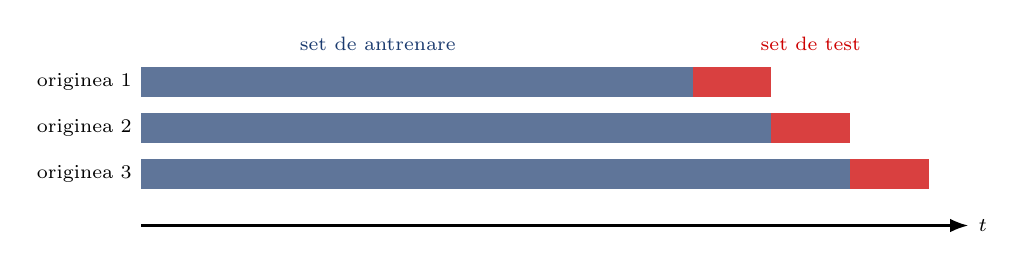
\begin{tikzpicture}[x=0.5cm, y=0.42cm, font=\scriptsize]
\foreach \r/\n in {0/1, 1/2, 2/3} {
  \pgfmathsetmacro{\e}{14 + 2*\r}
  \fill[MainBlue!70] (0, -\r*1.4) rectangle (\e, -\r*1.4 + 0.9);
  \fill[IDAred!75] (\e, -\r*1.4) rectangle (\e + 2, -\r*1.4 + 0.9);
  \node[left] at (0, -\r*1.4 + 0.45) {originea \n};
}
\node[text=MainBlue] at (6, 1.6) {set de antrenare};
\node[text=IDAred] at (17, 1.6) {set de test};
\draw[-{Latex}, thick] (0, -3.9) -- (21, -3.9) node[right] {$t$};
\end{tikzpicture}
\begin{itemize}
    \item \textbf{Împărțirea se face în timp, niciodată aleator}
    \begin{itemize}
        \item setul de antrenare: primele observații, folosite pentru alegerea și estimarea metodei
        \item setul de test: ultimele $h$ observații, ascunse și folosite doar pentru măsurarea erorilor
        \item o împărțire aleatoare îi permite modelului să vadă viitorul: erorile par prea mici
    \end{itemize}
    \item \textbf{Origine mobilă} (validare încrucișată pentru serii de timp): se repetă, mutînd originea înainte
    \begin{itemize}
        \item mediați erorile pe toate originile: o estimare mai stabilă a acurateței
    \end{itemize}
\end{itemize}
\end{frame}

\begin{frame}{Măsuri ale erorii de prognoză}
\itemsize{\footnotesize}
\begin{itemize}
    \item Erorile pe setul de test: $e_{T+j} = y_{T+j} - \hat y_{T+j|T}$, $j = 1, \ldots, h$
    \item \textbf{MAE} (mean absolute error, eroarea absolută medie) $= \frac1h \sum_j |e_{T+j}|$
    \begin{itemize}
        \item în unitățile seriei; ușor de explicat
    \end{itemize}
    \item \textbf{RMSE} (root mean squared error, rădăcina erorii pătratice medii) $= \sqrt{\frac1h \sum_j e_{T+j}^2}$
    \begin{itemize}
        \item penalizează mai mult erorile mari; întotdeauna $\ge$ MAE
    \end{itemize}
    \item \textbf{MAPE} (mean absolute percentage error, eroarea procentuală absolută medie) $= \frac{100}{h} \sum_j |e_{T+j} / y_{T+j}|$
    \begin{itemize}
        \item fără unități de măsură, dar inutilizabilă cînd $y$ este aproape de 0 (inflație, randamente)
    \end{itemize}
    \item \textbf{MASE} (mean absolute scaled error, eroarea absolută medie scalată) $=$ MAE $/$ MAE în eșantion a metodei naive sezoniere (\refHK)
    \begin{itemize}
        \item sub 1: mai bună decît metoda naivă sezonieră pe datele de antrenare; comparabilă între serii
    \end{itemize}
\end{itemize}
\end{frame}

\begin{frame}{Exemplu rezolvat: erorile calculate de mînă}
\itemsize{\footnotesize}
\begin{columns}[T]
\begin{column}{0.46\textwidth}
\begin{center}
\footnotesize
\begin{tabular}{lrrrr}
\toprule
& T1 & T2 & T3 & T4 \\
\midrule
anul 1 & 10 & 14 & 18 & 12 \\
anul 2 & 11 & 15 & 20 & 13 \\
\midrule anul 3 (test) & 12 & 16 & 21 & 14 \\
naivă & 13 & 13 & 13 & 13 \\
naivă sezonieră & 11 & 15 & 20 & 13 \\
\bottomrule
\end{tabular}
\end{center}

\end{column}
\begin{column}{0.50\textwidth}
\begin{itemize}
    \item \textbf{Naivă}: erorile $-1, 3, 8, 1$
    \begin{itemize}
        \item MAE $= (1 + 3 + 8 + 1)/4 = 3{,}25$
        \item RMSE $= \sqrt{(1 + 9 + 64 + 1)/4} = \sqrt{18{,}75} = 4{,}33$
    \end{itemize}
    \item \textbf{Naivă sezonieră}: erorile $1, 1, 1, 1$
    \begin{itemize}
        \item MAE $=$ RMSE $= 1$
    \end{itemize}
    \item \textbf{Interpretare}
    \begin{itemize}
        \item prognoza naivă ignoră sezonalitatea: eroarea ei mare din trimestrul III domină RMSE
        \item pentru datele sezoniere, metoda naivă sezonieră este reperul de depășit
    \end{itemize}
\end{itemize}
\end{column}
\end{columns}
\end{frame}

\begin{frame}{Prognoza producției de electricitate}
\itemsize{\footnotesize}
\begin{center}
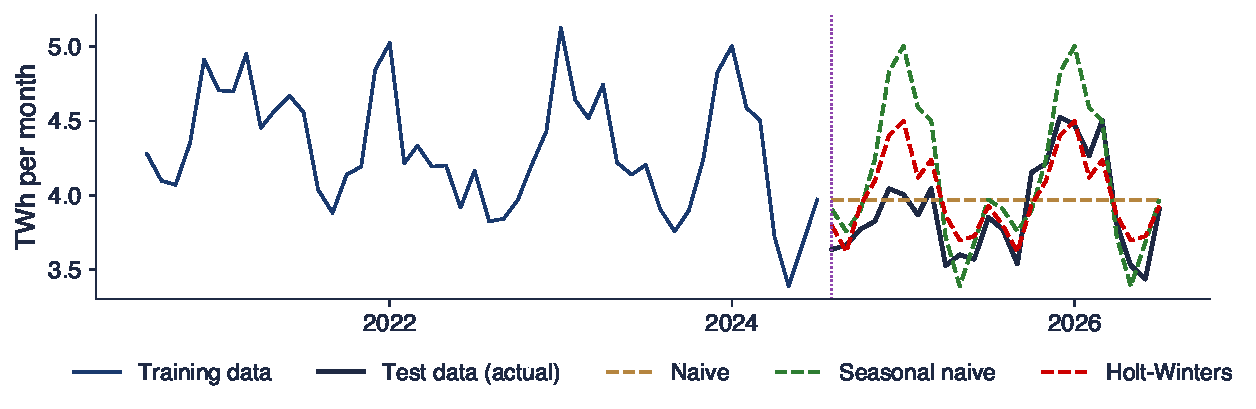
\includegraphics[width=0.94\textwidth,height=0.58\textheight,keepaspectratio]{tsa_ch0_forecast.pdf}
\end{center}
\vspace{-2mm}
\begin{itemize}
    \item Setul de test: august 2024 -- iulie 2026 (24 de luni); datele de antrenare: toate lunile anterioare; linii întrerupte: prognoze făcute o singură dată, la sfîrșitul setului de antrenare
\end{itemize}
\quantlet{TSA\_ch0\_forecast}{\qlurl{TSA_ch0_forecast}}
\end{frame}

\begin{frame}{Interpretarea: metoda cîștigătoare}
\itemsize{\footnotesize}
\begin{columns}[T]
\begin{column}{0.50\textwidth}
\begin{center}
\scriptsize
\begin{tabular}{lrrrr}
\toprule
\textbf{Metodă} & MAE & RMSE & MAPE & MASE \\
\midrule
Naivă & 0{,}28 & 0{,}33 & 7{,}3\% & 0{,}82 \\
Naivă sezonieră & 0{,}28 & 0{,}38 & 7{,}2\% & 0{,}83 \\
SES & 0{,}28 & 0{,}32 & 7{,}1\% & 0{,}81 \\
Holt--Winters & 0{,}17 & 0{,}21 & 4{,}5\% & 0{,}51 \\
\bottomrule
\end{tabular}
\end{center}
\begin{itemize}
    \item MAE și RMSE în TWh pe lună
\end{itemize}
\end{column}
\begin{column}{0.46\textwidth}
\begin{itemize}
    \item \textbf{Holt--Winters} are cea mai mică eroare după fiecare măsură
    \begin{itemize}
        \item combină nivelul în scădere cu vîrful de iarnă
    \end{itemize}
    \item \textbf{Aici, metoda naivă sezonieră nu este mai bună decît cea naivă}
    \begin{itemize}
        \item copiază iarna puternică din 2023--2024 peste perioada 2024--2026, cu un nivel mai scăzut
    \end{itemize}
    \item O singură perioadă de test de 24 de luni este un singur eșantion: o origine mobilă oferă un răspuns mai solid
\end{itemize}
\end{column}
\end{columns}
\end{frame}

\begin{frame}{Studiu de caz: competiția M4}
\itemsize{\footnotesize}
\begin{itemize}
    \item \textbf{Întrebarea}: ce metode de prognoză funcționează cel mai bine pe date reale?
    \begin{itemize}
        \item competițiile M, inițiate de Spyros Makridakis în 1982: prognozele sînt trimise fără acces la datele de test și sînt evaluate pe acestea
    \end{itemize}
    \item \textbf{M4 (2018)}: 100\,000 de serii (de la anuale la orare), 61 de metode (\refMfour)
    \begin{itemize}
        \item 12 dintre cele mai precise 17 metode au fost \textbf{combinații} de metode
        \item cîștigătoarea a fost o metodă hibridă, care combină netezirea exponențială cu o rețea neuronală
        \item metodele care folosesc exclusiv învățarea automată au avut rezultate slabe: niciuna nu a depășit o combinație simplă de metode de netezire exponențială
    \end{itemize}
    \item \textbf{Relevanța pentru acest curs}
    \begin{itemize}
        \item întîi metodele de referință; acuratețea se măsoară în afara eșantionului, pe multe serii, nu pe una singură
        \item aceeași lecție apăruse și în M3 (\refMthree): o metodă complexă nu este automat mai bună
    \end{itemize}
\end{itemize}
\end{frame}

\begin{frame}{O mică competiție M pe date românești}
\itemsize{\footnotesize}
\begin{center}
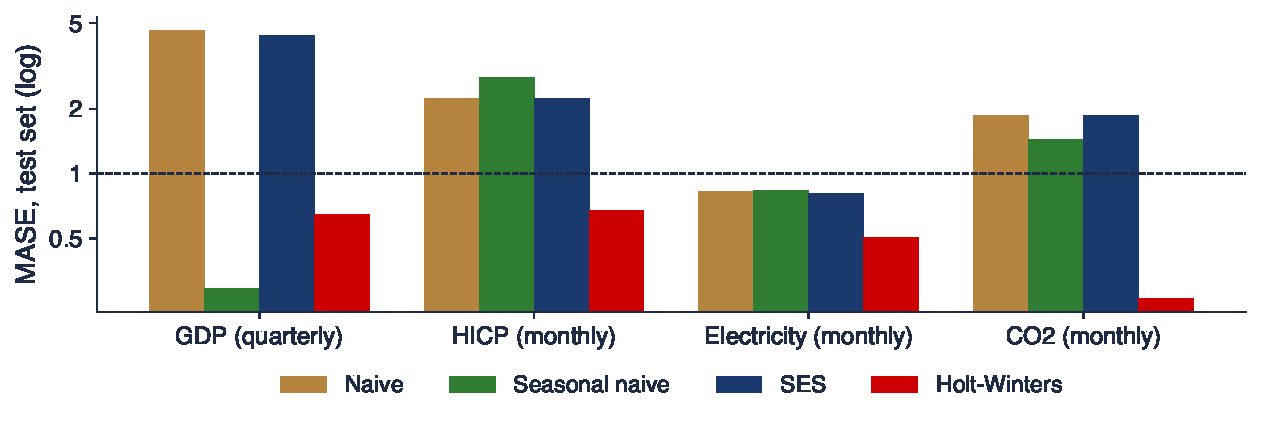
\includegraphics[width=0.94\textwidth,height=0.56\textheight,keepaspectratio]{tsa_ch0_benchmarks.pdf}
\end{center}
\vspace{-2mm}
\begin{itemize}
    \item MASE pe setul de test (scară logaritmică) pentru patru metode și patru serii sezoniere; seturi de test: ultimele 8 trimestre (PIB) sau 24 de luni; linia întreruptă: MASE = 1
\end{itemize}
\quantlet{TSA\_ch0\_forecast}{\qlurl{TSA_ch0_forecast}}
\end{frame}

\begin{frame}{Interpretarea: mini-competiția}
\itemsize{\small}
\begin{itemize}
    \item \textbf{Holt--Winters cîștigă pe 3 din 4 serii}
    \begin{itemize}
        \item CO2: MASE 0{,}26, față de 1{,}45 pentru metoda naivă sezonieră; IAPC: 0{,}68, față de 2{,}24 pentru cea naivă
    \end{itemize}
    \item \textbf{PIB: cîștigă metoda naivă sezonieră}, MASE 0{,}29 față de 0{,}65
    \begin{itemize}
        \item creșterea s-a oprit în 2025--2026: trendul estimat de Holt--Winters duce la prognoze prea mari
    \end{itemize}
    \item \textbf{Metodele naivă și SES eșuează pe seriile sezoniere}
    \begin{itemize}
        \item PIB: MASE 4{,}62 (naivă) și 4{,}39 (SES): ignoră sezonalitatea
    \end{itemize}
    \item Ca în M4: nicio metodă nu cîștigă peste tot, iar o metodă de referință simplă poate depăși un model aparent mai bun
\end{itemize}
\end{frame}

\begin{frame}{Recapitulare: prognoza și evaluarea ei}
\itemsize{\small}
\begin{itemize}
    \item $\hat y_{T+h|T}$ folosește doar informația pînă la $T$; incertitudinea crește odată cu $h$
    \item Metode de referință: media, naivă, naivă sezonieră, cu derivă
    \item Împărțiți datele în timp; măsurați MAE, RMSE, MAPE și MASE doar pe setul de test
    \item M4 și mini-competiția noastră: metodele simple sînt puternice; combinațiile și Holt--Winters au rezultate bune
\end{itemize}
\end{frame}


%=============================================================================
\section{Instrumente}
%=============================================================================

\begin{frame}{Python pentru serii de timp}
\itemsize{\small}
\begin{itemize}
    \item \textbf{Bibliotecile cursului}
    \begin{itemize}
        \item \textbf{NumPy}: tablouri și algebră liniară (\refNumpy)
        \item \textbf{pandas}: tabele indexate după dată, schimbarea frecvenței, laguri, diferențe (\refPandas)
        \item \textbf{matplotlib}: grafice
        \item \textbf{statsmodels}: descompunere, netezire exponențială, ARIMA, VAR, teste de rădăcină unitară (\refStatsmodels)
        \item \textbf{arch}: modele GARCH (\tsachlink{https://danpele.github.io/Time-Series-Analysis/RO/Cursuri/capitol5_volatilitate_conditionata_garch.pdf}{Capitolul 5})
    \end{itemize}
    \item \textbf{Google Colab}: notebook-uri în browser, fără instalare
    \begin{itemize}
        \item deschideți un notebook al cursului cu un singur clic; \emph{File $\to$ Save a copy in Drive} vă păstrează modificările
        \item fiecare grafic din slide-uri are un Quantlet: același cod, care poate fi rulat în Colab
    \end{itemize}
\end{itemize}
\end{frame}

\begin{frame}[fragile]{Primul script}
\itemsize{\scriptsize}
\begin{columns}[T]
\begin{column}{0.62\textwidth}
\begin{lstlisting}
import pandas as pd
from statsmodels.tsa.seasonal import seasonal_decompose
from statsmodels.tsa.holtwinters import ExponentialSmoothing

# Romanian real GDP, quarterly (Eurostat)
url = ('https://ec.europa.eu/eurostat/api/dissemination/'
       'sdmx/2.1/data/namq_10_gdp/Q.CLV10_MEUR.NSA.B1GQ.RO'
       '?format=SDMX-CSV')
t = pd.read_csv(url)
y = pd.Series(t['OBS_VALUE'].values / 1000,
              index=pd.PeriodIndex(t['TIME_PERIOD'], freq='Q'))
y = y.to_timestamp()

dec = seasonal_decompose(y, model='multiplicative', period=4)
print(dec.seasonal.iloc[:4])            # seasonal factors
yoy = 100 * (y / y.shift(4) - 1)         # annual growth, %
hw = ExponentialSmoothing(y, trend='add', seasonal='mul',
                          seasonal_periods=4).fit()
print(hw.forecast(4))                    # next four quarters
\end{lstlisting}
\end{column}
\begin{column}{0.35\textwidth}
\begin{itemize}
    \item \textbf{Linie cu linie}
    \item citirea seriei direct din API-ul Eurostat (fără cheie)
    \item \texttt{PeriodIndex}: trimestrele ca indice de timp
    \item descompunere clasică multiplicativă, cu $m = 4$
    \item \texttt{shift(4)}: valoarea din același trimestru al anului anterior
    \item Holt--Winters cu trend aditiv și sezonalitate multiplicativă
    \item API (application programming interface): interfață de programare a aplicațiilor
\end{itemize}
\end{column}
\end{columns}
\end{frame}


%=============================================================================
\section{Contribuția posibilă a AI}
%=============================================================================

\begin{frame}{Contribuția posibilă a AI}
\itemsize{\small}
\begin{itemize}
    \item \textbf{Unde ajută un asistent AI}
    \begin{itemize}
        \item o primă variantă a codului care citește și reprezintă grafic o serie Eurostat sau BNR
        \item explicarea unui mesaj de eroare sau a unei funcții statsmodels
        \item enumerarea explicațiilor posibile ale unui tipar (o scădere a PIB, un salt al cursului EUR/RON)
    \end{itemize}
    \item \textbf{Greșeli frecvente în codul generat de AI pentru serii de timp}
    \begin{itemize}
        \item împărțirea aleatoare în set de antrenare și set de test, care îi permite modelului să vadă viitorul
        \item creșterea pe un trimestru numită „creștere anuală”; \texttt{shift(1)} în loc de \texttt{shift(4)}
        \item RMSE fără rădăcina pătrată; MAPE pe o serie care trece prin zero
    \end{itemize}
    \item Seminarul 0, exercițiul C2: găsiți trei astfel de greșeli într-un răspuns generat de AI
\end{itemize}
\end{frame}

\begin{frame}{Verificări necesare}
\itemsize{\small}
\begin{itemize}
    \item \textbf{Datele}
    \begin{itemize}
        \item reprezentați seria grafic înainte de orice calcul; verificați frecvența, unitățile de măsură, prima și ultima dată
        \item ajustată sau neajustată? Un model pentru sezonalitate are nevoie de seria neajustată
    \end{itemize}
    \item \textbf{Evaluarea}
    \begin{itemize}
        \item setul de test urmează după setul de antrenare; se folosește o singură dată, la final
        \item comparați cu prognozele naivă și naivă sezonieră înainte de a declara un succes
    \end{itemize}
    \item \textbf{Afirmațiile}
    \begin{itemize}
        \item fiecare referință: deschideți DOI-ul; fiecare rezultat numeric: recalculați-l
        \item declarați utilizarea AI în \texttt{AI\_USE.md}
    \end{itemize}
\end{itemize}
\end{frame}


%=============================================================================
\section{Concluzii}
%=============================================================================

\begin{frame}{Idei de reținut}
\itemsize{\small}
\begin{itemize}
    \item Nota: 70\% examen, 20\% proiect, 10\% prezență; AI permis și declarat; seminariile înaintea cursurilor
    \item O serie de timp este ordonată în timp; dependența de trecut face posibilă prognoza
    \item Componente: trend, sezonalitate (perioadă fixă), ciclu (fără perioadă fixă), componenta neregulată; aditiv sau multiplicativ
    \item Yule și Slutsky: dependența și sumele de șocuri, originile modelelor AR și MA
    \item ACF dezvăluie trendul (descreștere lentă), sezonalitatea (vîrfuri la $m$) și memoria
    \item Netezirea exponențială acordă ponderi mai mari trecutului recent; evaluați orice prognoză față de metodele naive, pe un set de test
\end{itemize}
\end{frame}

\begin{frame}{Autoevaluare, idee de proiect; urmează \tsachlinkt{https://danpele.github.io/Time-Series-Analysis/RO/Cursuri/capitol1_procese_stochastice_stationaritate.pdf}{Capitolul 1}}
\itemsize{\footnotesize}
\begin{columns}[T]
\begin{column}{0.52\textwidth}
\begin{itemize}
    \item \textbf{Autoevaluare}
    \begin{itemize}
        \item De ce este înșelătoare creșterea față de trimestrul anterior a PIB-ului neajustat?
        \item Ce înseamnă un factor sezonier de 0,76 pentru trimestrul I?
        \item Ce spune despre o serie o valoare estimată a lui $\alpha$ apropiată de 1?
        \item De ce trebuie ca setul de test să urmeze după setul de antrenare?
    \end{itemize}
    \item \textbf{Idee de proiect}
    \begin{itemize}
        \item prognozați producția lunară de electricitate a României cu un an înainte; comparați metoda naivă sezonieră, Holt--Winters și STL urmată de SES, cu origine mobilă
    \end{itemize}
\end{itemize}
\end{column}
\begin{column}{0.44\textwidth}
\begin{itemize}
    \item \textbf{\tsachlink{https://danpele.github.io/Time-Series-Analysis/RO/Cursuri/capitol1_procese_stochastice_stationaritate.pdf}{Capitolul 1}: procese stochastice și staționaritate}
    \begin{itemize}
        \item Ce este un proces stochastic?
        \item Cînd are o serie medie și varianță stabile?
        \item Ce sînt zgomotul alb și mersul aleator?
        \item Cum testăm că autocorelațiile sînt nule?
    \end{itemize}
\end{itemize}
\end{column}
\end{columns}
\end{frame}


%=============================================================================
\section{Bibliografie}
%=============================================================================

\begin{frame}{Bibliografie (1/2)}
\itemsize{\tiny}
\begin{itemize}
    \item Box, G.E.P., Jenkins, G.M. (1970). \emph{Time Series Analysis: Forecasting and Control}. Holden-Day; 4th ed.\ with G.C.\ Reinsel: \href{https://doi.org/10.1002/9781118619193}{Wiley (2008)}.
    \item Brockwell, P.J., Davis, R.A. (2016). \href{https://doi.org/10.1007/978-3-319-29854-2}{\emph{Introduction to Time Series and Forecasting}} (3rd ed.). Springer.
    \item Cleveland, R.B., Cleveland, W.S., McRae, J.E., Terpenning, I. (1990). \href{https://www.scb.se/contentassets/ca21efb41fee47d293bbee5bf7be7fb3/stl-a-seasonal-trend-decomposition-procedure-based-on-loess.pdf}{STL: a seasonal-trend decomposition procedure based on loess}. \emph{Journal of Official Statistics}, 6(1), 3--73.
    \item Engle, R.F. (1982). \href{https://doi.org/10.2307/1912773}{Autoregressive conditional heteroscedasticity with estimates of the variance of United Kingdom inflation}. \emph{Econometrica}, 50(4), 987--1007.
    \item Engle, R.F., Granger, C.W.J. (1987). \href{https://doi.org/10.2307/1913236}{Co-integration and error correction: representation, estimation, and testing}. \emph{Econometrica}, 55(2), 251--276.
    \item Gardner, E.S. (1985). \href{https://doi.org/10.1002/for.3980040103}{Exponential smoothing: the state of the art}. \emph{Journal of Forecasting}, 4(1), 1--28.
    \item Hamilton, J.D. (1994). \href{https://doi.org/10.2307/j.ctv14jx6sm}{\emph{Time Series Analysis}}. Princeton University Press.
    \item Harris, C.R., Millman, K.J., van der Walt, S.J., et al.\ (2020). \href{https://doi.org/10.1038/s41586-020-2649-2}{Array programming with NumPy}. \emph{Nature}, 585, 357--362.
    \item Holt, C.C. (1957; reprinted 2004). \href{https://doi.org/10.1016/j.ijforecast.2003.09.015}{Forecasting seasonals and trends by exponentially weighted moving averages}. \emph{International Journal of Forecasting}, 20(1), 5--10.
    \item Huang, C., Petukhina, A. (2022). \href{https://doi.org/10.1007/978-3-031-13584-2}{\emph{Applied Time Series Analysis and Forecasting with Python}}. Springer.
    \item Hyndman, R.J., Athanasopoulos, G. (2021). \href{https://otexts.com/fpp3/}{\emph{Forecasting: Principles and Practice}} (3rd ed.). OTexts.
    \item Hyndman, R.J., Koehler, A.B. (2006). \href{https://doi.org/10.1016/j.ijforecast.2006.03.001}{Another look at measures of forecast accuracy}. \emph{International Journal of Forecasting}, 22(4), 679--688.
    \item Hyndman, R.J., Koehler, A.B., Snyder, R.D., Grose, S. (2002). \href{https://doi.org/10.1016/S0169-2070(01)00110-8}{A state space framework for automatic forecasting using exponential smoothing methods}. \emph{International Journal of Forecasting}, 18(3), 439--454.
\end{itemize}
\end{frame}

\begin{frame}{Bibliografie (2/2)}
\itemsize{\tiny}
\begin{itemize}
    \item Keeling, C.D. (1960). \href{https://doi.org/10.3402/tellusa.v12i2.9366}{The concentration and isotopic abundances of carbon dioxide in the atmosphere}. \emph{Tellus}, 12(2), 200--203.
    \item Kolmogorov, A.N. (1941). Interpolation and extrapolation of stationary random sequences. English translation in \href{https://doi.org/10.1007/978-94-011-2260-3_28}{\emph{Selected Works of A.N.\ Kolmogorov}, Vol.\ II}, Springer (1992), 272--280.
    \item Makridakis, S., Hibon, M. (2000). \href{https://doi.org/10.1016/S0169-2070(00)00057-1}{The M3-Competition: results, conclusions and implications}. \emph{International Journal of Forecasting}, 16(4), 451--476.
    \item Makridakis, S., Spiliotis, E., Assimakopoulos, V. (2020). \href{https://doi.org/10.1016/j.ijforecast.2019.04.014}{The M4 Competition: 100,000 time series and 61 forecasting methods}. \emph{International Journal of Forecasting}, 36(1), 54--74.
    \item McKinney, W. (2010). \href{https://doi.org/10.25080/Majora-92bf1922-00a}{Data structures for statistical computing in Python}. \emph{Proceedings of the 9th Python in Science Conference}, 56--61.
    \item Seabold, S., Perktold, J. (2010). \href{https://doi.org/10.25080/Majora-92bf1922-011}{Statsmodels: econometric and statistical modeling with Python}. \emph{Proceedings of the 9th Python in Science Conference}, 92--96.
    \item Sims, C.A. (1980). \href{https://doi.org/10.2307/1912017}{Macroeconomics and reality}. \emph{Econometrica}, 48(1), 1--48.
    \item Slutzky, E. (1937). \href{https://doi.org/10.2307/1907241}{The summation of random causes as the source of cyclic processes}. \emph{Econometrica}, 5(2), 105--146.
    \item Wiener, N. (1949). \href{https://doi.org/10.7551/mitpress/2946.001.0001}{\emph{Extrapolation, Interpolation, and Smoothing of Stationary Time Series}}. MIT Press.
    \item Winters, P.R. (1960). \href{https://doi.org/10.1287/mnsc.6.3.324}{Forecasting sales by exponentially weighted moving averages}. \emph{Management Science}, 6(3), 324--342.
    \item Yule, G.U. (1926). \href{https://doi.org/10.2307/2341482}{Why do we sometimes get nonsense-correlations between time-series?} \emph{Journal of the Royal Statistical Society}, 89(1), 1--63.
    \item Yule, G.U. (1927). \href{https://doi.org/10.1098/rsta.1927.0007}{On a method of investigating periodicities in disturbed series, with special reference to Wolfer's sunspot numbers}. \emph{Philosophical Transactions of the Royal Society A}, 226, 267--298.
\end{itemize}
\end{frame}

\end{document}
